% Plik pomocniczy: podgląd wzoru całej pracy (bez strony tytułowej) poza szablonem PG.
% Kompilacja w folderze praca/wzor: pdflatex wzor_podglad; bibtex wzor_podglad; pdflatex ×2.
% W docelowej pracy wstaw pliki przez \input{wzor/...} w szablonie PG; potrzebne pakiety i polskie
% nazwy dla algorytmów i listingów skopiuj z preambuły poniżej.
\documentclass[12pt,a4paper]{report}
\usepackage[T1]{fontenc}
\usepackage[utf8]{inputenc}
% \usepackage{lmodern} % odkomentuj, jeśli masz pakiet lmodern
\usepackage[provide=*]{babel}
\babelprovide[import,main]{polish}
\usepackage[a4paper,margin=2.5cm]{geometry}
\usepackage{graphicx}
\usepackage{booktabs}
\usepackage{tabularx}
\usepackage{longtable}
\usepackage{makecell}
\usepackage{amsmath}
\usepackage{textcomp}
\usepackage[chapter]{algorithm} % numeracja algorytmów w rozdziale (5.1, 5.2)
\usepackage[noend]{algpseudocode}
\usepackage{listings}
\usepackage[hidelinks]{hyperref}
\graphicspath{{../}}

% --- polskie nazwy: algorytmy (pakiety algorithm, algpseudocode) ---
\floatname{algorithm}{Algorytm}
\renewcommand{\listalgorithmname}{Spis algorytmów}
\algrenewcommand\algorithmicrequire{\textbf{Wejście:}}
\algrenewcommand\algorithmicensure{\textbf{Wyjście:}}
\algrenewcommand\algorithmicfor{\textbf{dla}}
\algrenewcommand\algorithmicforall{\textbf{dla wszystkich}}
\algrenewcommand\algorithmicdo{\textbf{wykonaj}}
\algrenewcommand\algorithmicif{\textbf{jeżeli}}
\algrenewcommand\algorithmicthen{\textbf{to}}
\algrenewcommand\algorithmicelse{\textbf{w przeciwnym razie}}
\algrenewcommand\algorithmicreturn{\textbf{zwróć}}
\algrenewcommand{\algorithmiccomment}[1]{\hfill$\triangleright$~#1}
% --- listingi (pakiet listings) ---
\renewcommand{\lstlistingname}{Listing}
\renewcommand{\lstlistlistingname}{Spis listingów}
\lstset{basicstyle=\ttfamily\footnotesize, frame=single, columns=fullflexible, keepspaces=true,
        breaklines=true, captionpos=t}

\begin{document}
% =====================================================================
% Streszczenie i Abstract (WZÓR) – w szablonie PG wstaw w przeznaczone miejsca (przed spisem treści).
% Słowa kluczowe: 5–6; dziedzina OECD – sprawdź listę w szablonie PG.
% W tekście angielskim kropka dziesiętna. Plan: materialy/07_plan_dodatki_streszczenie_skroty.md.
% =====================================================================

\chapter*{Streszczenie}
\addcontentsline{toc}{chapter}{Streszczenie}

Termografia może uzupełniać ocenę zmian skórnych na zdjęciach o informację o rozkładzie temperatury skóry, ale wspólna analiza obu obrazów wymaga ich rejestracji. Zdjęcie z telefonu i obraz termowizyjny pochodzą z niezależnych urządzeń, a znamię bez schłodzenia skóry nie jest widoczne na termogramie. Celem pracy było opracowanie, implementacja oraz ocena systemu, który rejestruje zdjęcie RGB i obraz termowizyjny zmiany skórnej, przenosi obszar zainteresowania między modalnościami, wyznacza jego parametry ilościowe i weryfikuje zgodność obszaru za pomocą modeli segmentacji dedykowanych każdej modalności. Zaprojektowano znacznik referencyjny w kształcie litery $\Pi$, widoczny w obu modalnościach, i metodę rejestracji maksymalizującą kryterium ECC na maskach znacznika. Znamię na zdjęciu segmentuje model PanDerm z dekoderem UperNet douczony na zbiorze ISIC 2018, a znacznik na obrazie termowizyjnym -- sieć U-Net uczona na danych własnych. System wyznacza wymiary znamienia w milimetrach, miary zgodności masek oraz współrzędne i surową intensywność pikseli obrazu termowizyjnego w obszarze znamienia, a wyniki zapisuje w raporcie i bazie danych SQLite. Weryfikację przeprowadzono na 94 parach obrazów 34 znamion. Mediana błędu rejestracji wyniosła 0,61~mm (w 85\% par nie więcej niż 1~mm), wobec 3,36~mm dla rejestracji z użyciem informacji wzajemnej. Sieć U-Net uzyskała współczynnik Dice'a 0,969, a model PanDerm na zdjęciach z telefonu -- 0,870. Zgodność masek znacznika między modalnościami, wyznaczana bez adnotacji (Dice 0,957), była silnie skorelowana z błędem rejestracji, co pozwala wskazywać pary wymagające sprawdzenia.

\vspace{1em}
\noindent\textbf{Słowa kluczowe:} rejestracja obrazów wielomodalnych, termowizja, segmentacja obrazów medycznych, znamię barwnikowe, znacznik referencyjny, uczenie głębokie.

\noindent\textbf{Dziedzina nauki i techniki, zgodnie z wymogami OECD:} nauki inżynieryjne i techniczne, inżynieria medyczna. % TODO: sprawdzić brzmienie w szablonie PG

\chapter*{Abstract}
\addcontentsline{toc}{chapter}{Abstract}

Thermal imaging can complement the assessment of skin lesions in photographs with information on skin temperature distribution, but a joint analysis of both images requires their registration. A smartphone photograph and a thermal image come from independent devices, and a nevus is not visible in a thermogram unless the skin is cooled. The aim of this thesis was to design, implement and evaluate a system that registers an RGB photograph and a thermal image of a skin lesion, transfers the region of interest between the modalities, computes its quantitative parameters, and verifies the agreement of the region using segmentation models dedicated to each modality. A $\Pi$-shaped fiducial marker visible in both modalities was designed, together with a registration method that maximizes the enhanced correlation coefficient (ECC) on marker masks. The nevus in the photograph is segmented by the PanDerm foundation model with an UperNet decoder fine-tuned on the ISIC 2018 dataset, and the marker in the thermal image by a U-Net trained on the author's data. The system measures the lesion in millimeters, computes mask agreement metrics, and exports the coordinates and raw intensity of every thermal image pixel within the lesion; the results are stored in a report and an SQLite database. The system was evaluated on 94 image pairs of 34 nevi. The median target registration error was 0.61~mm (at most 1~mm in 85\% of pairs), compared with 3.36~mm for mutual information registration. The U-Net achieved a Dice coefficient of 0.969, and PanDerm achieved 0.870 on smartphone photographs. The agreement of marker masks between modalities, computed without annotations (Dice 0.957), was strongly correlated with the registration error, which allows pairs requiring inspection to be identified.

\vspace{1em}
\noindent\textbf{Keywords:} multimodal image registration, thermal imaging, medical image segmentation, melanocytic nevus, fiducial marker, deep learning.

\noindent\textbf{Field of science and technology in accordance with OECD requirements:} engineering and technology, medical engineering. % TODO: sprawdzić w szablonie PG

\tableofcontents
% =====================================================================
% Wykaz ważniejszych oznaczeń i skrótów (WZÓR) – w szablonie PG wstaw w przeznaczone miejsce
% (zwykle po spisie treści). Zawiera tylko skróty i oznaczenia użyte w rozdziałach 1–7 i dodatkach wzoru.
% Wymaga pakietu longtable. Nazwy własne (PanDerm, OpenCV, SQLite) i nazwy zbiorów danych bez rozwinięcia
% nie są skrótami – pominięto je. Przy pierwszym użyciu w tekście skrót i tak należy rozwinąć.
% =====================================================================

\chapter*{Wykaz ważniejszych oznaczeń i skrótów}
\addcontentsline{toc}{chapter}{Wykaz ważniejszych oznaczeń i skrótów}

\subsection*{Oznaczenia}

{\small
\begin{longtable}{@{}p{2.6cm}p{12.2cm}@{}}
  $A$, $B$ & porównywane maski; w badaniu E2: $A$ -- maska przeniesiona ze zdjęcia, $B$ -- maska wyznaczona na obrazie termowizyjnym \\
  $|A|$ & pole maski $A$ \\
  $d$ & średnica równoważna znamienia \\
  $e$ & średni błąd krawędzi masek znacznika \\
  $G_\sigma$ & filtr Gaussa o odchyleniu standardowym $\sigma$ \\
  $H$, $H_T$ & homografia przekształcająca piksele obrazu na milimetry w płaszczyźnie znacznika; $H_T$ -- dla obrazu termowizyjnego \\
  $I$ & surowa wartość detektora (intensywność) piksela obrazu termowizyjnego \\
  $L$, $P$ & obwód i pole znamienia \\
  $M_R$, $M_T$ & maska znacznika na zdjęciu i na obrazie termowizyjnym \\
  $p_i^R$, $p_i^T$ & $i$-ty narożnik znacznika na zdjęciu i na obrazie termowizyjnym \\
  P1--P8 & narożniki znacznika $\Pi$ \\
  $T$ & macierz rejestracji 3~$\times$~3 (piksel zdjęcia $\to$ piksel obrazu termowizyjnego) \\
  $u$ & ułamek pola piksela pokryty przez znamię \\
  $W_0$, $W_A$, $W_H$ & przekształcenie: wstępne (podobieństwo), afiniczne, homografia \\
  $x$, $y$ & współrzędne piksela: kolumna i wiersz \\
  $\eta$ & współczynnik uczenia \\
  $\varepsilon$ & próg zbieżności metody ECC \\
  $\lambda$ & współczynnik regularyzacji wag (ang.~\textit{weight decay}) \\
  $\Pi$ & znacznik referencyjny w kształcie litery $\Pi$ \\
  $\rho$ & współczynnik korelacji rang Spearmana \\
  $\sigma$ & odchylenie standardowe; parametr rozmycia filtrem Gaussa \\
  j.s. & jednostki surowe detektora kamery termowizyjnej \\
\end{longtable}
}

\subsection*{Skróty}

{\small
\begin{longtable}{@{}p{2.6cm}p{12.2cm}@{}}
  ASSD & średnia symetryczna odległość konturów (ang.~\textit{average symmetric surface distance}) \\
  BCE & binarna entropia krzyżowa (ang.~\textit{binary cross-entropy}) \\
  CSV & plik tekstowy z wartościami rozdzielonymi separatorem (ang.~\textit{comma-separated values}) \\
  CUDA & platforma obliczeń równoległych na procesorach graficznych (ang.~\textit{Compute Unified Device Architecture}) \\
  CVAT & program do adnotacji obrazów (ang.~\textit{Computer Vision Annotation Tool}) \\
  DSC & współczynnik Dice'a (ang.~\textit{Dice similarity coefficient}) \\
  E1, E2, E4 & badania weryfikacyjne: E1 -- dokładność rejestracji względem adnotacji, E2 -- zgodność masek znacznika między modalnościami bez adnotacji, E4 -- porównanie metod rejestracji \\
  ECC & rozszerzony współczynnik korelacji (ang.~\textit{enhanced correlation coefficient}) \\
  FLE & błąd lokalizacji znacznika (ang.~\textit{fiducial localization error}) \\
  FPN & piramidalna sieć cech (ang.~\textit{Feature Pyramid Network}) \\
  FRE & błąd dopasowania znaczników (ang.~\textit{fiducial registration error}) \\
  GPU & procesor graficzny (ang.~\textit{graphics processing unit}) \\
  HD95 & 95. percentyl odległości Hausdorffa (ang.~\textit{95th percentile Hausdorff distance}) \\
  HEIC & format zapisu zdjęć (ang.~\textit{High Efficiency Image Container}) \\
  HTML & język znaczników dokumentów internetowych (ang.~\textit{HyperText Markup Language}) \\
  IoU & indeks Jaccarda -- iloraz części wspólnej i sumy obszarów (ang.~\textit{intersection over union}) \\
  ISBI & międzynarodowe sympozjum obrazowania biomedycznego (ang.~\textit{International Symposium on Biomedical Imaging}) \\
  ISIC & międzynarodowa współpraca w zakresie obrazowania skóry (ang.~\textit{International Skin Imaging Collaboration}) \\
  JAC & indeks Jaccarda (ang.~\textit{Jaccard index}) \\
  JPG & format stratnej kompresji obrazów (ang.~\textit{Joint Photographic Experts Group}) \\
  JSON & tekstowy format wymiany danych (ang.~\textit{JavaScript Object Notation}) \\
  M1 & model segmentacji znamienia na zdjęciu (PanDerm z dekoderem UperNet) \\
  M3 & model segmentacji znacznika na obrazie termowizyjnym (U-Net) \\
  MI & informacja wzajemna (ang.~\textit{mutual information}) \\
  MR & rezonans magnetyczny (ang.~\textit{magnetic resonance}) \\
  NIR & bliska podczerwień (ang.~\textit{near infrared}) \\
  NMI & znormalizowana informacja wzajemna (ang.~\textit{normalized mutual information}) \\
  OECD & Organizacja Współpracy Gospodarczej i Rozwoju (ang.~\textit{Organisation for Economic Co-operation and Development}) \\
  ONNX & otwarty format zapisu modeli sieci neuronowych (ang.~\textit{Open Neural Network Exchange}) \\
  PNG & format bezstratnej kompresji obrazów (ang.~\textit{Portable Network Graphics}) \\
  PPM & moduł łączenia piramidalnego (ang.~\textit{Pyramid Pooling Module}) \\
  PU & przypadek użycia \\
  ReLU & funkcja aktywacji -- jednostka liniowa z obcięciem (ang.~\textit{rectified linear unit}) \\
  RGB & model barw: czerwony, zielony, niebieski; w pracy -- zdjęcie w świetle widzialnym (ang.~\textit{red, green, blue}) \\
  ROI & obszar zainteresowania (ang.~\textit{region of interest}) \\
  SEQ & format nagrań kamer termowizyjnych FLIR (sekwencja klatek z danymi radiometrycznymi) \\
  SQL & strukturalny język zapytań (ang.~\textit{Structured Query Language}) \\
  SSIM & indeks podobieństwa strukturalnego (ang.~\textit{structural similarity index}) \\
  SURF & przyspieszone odporne cechy (ang.~\textit{Speeded-Up Robust Features}) \\
  T01--T18 & testy funkcjonalne systemu \\
  TG1--TG6 & testy interfejsu graficznego \\
  TH & obraz termowizyjny (ang.~\textit{thermal}) \\
  TRE & błąd w punkcie docelowym (ang.~\textit{target registration error}) \\
  TRUS & ultrasonografia przezodbytnicza (ang.~\textit{transrectal ultrasound}) \\
  UML & ujednolicony język modelowania (ang.~\textit{Unified Modeling Language}) \\
  ViT & transformer wizyjny (ang.~\textit{Vision Transformer}); ViT-L -- wariant duży \\
  VIS & światło widzialne (ang.~\textit{visible}) \\
  WF & wymaganie funkcjonalne \\
  WN & wymaganie pozafunkcjonalne \\
\end{longtable}
}

% =====================================================================
% Rozdział 1 – Wstęp (WZÓR, ok. 2 strony)
% Styl bezosobowy. Klucze \cite{} – plik literatura_wzor.bib.
% Rysunek: ../rysunki/para_14_rgb_termowizja.pdf (ścieżki względem folderu praca/).
% Fragmenty oznaczone "% TODO" wymagają sprawdzenia albo decyzji autora.
% =====================================================================

\chapter{Wstęp}
\label{chap:wstep}

\section{Motywacja}
\label{sec:motywacja}

Czerniak jest jednym z najgroźniejszych nowotworów skóry, a jego wczesne wykrycie decyduje o skuteczności leczenia. W ocenie zmian barwnikowych podstawową rolę odgrywa obraz w świetle widzialnym -- zdjęcie kliniczne lub obraz dermatoskopowy -- na którym ocenia się kształt, brzeg i barwę zmiany~\cite{dermoscopy}. Obraz taki nie niesie jednak informacji o procesach fizjologicznych zachodzących w zmianie.

Informację tę może uzupełnić termografia, czyli rejestracja promieniowania podczerwonego emitowanego przez skórę. Skóra zachowuje się niemal jak ciało doskonale czarne o emisyjności 0,96--0,98, dzięki czemu termogram odwzorowuje rozkład temperatury jej powierzchni~\cite{infared-thermal-imaging}. Zmiany nowotworowe mogą różnić się od otoczenia odpowiedzią termiczną, zwłaszcza po kontrolowanym schłodzeniu skóry~\cite{visualization-detection-cancer,magalhaes2019}. Obraz widzialny i obraz termowizyjny mają więc charakter komplementarny: pierwszy zawiera bogatą teksturę, drugi -- informację termiczną, ubogą jednak w szczegóły~\cite{deep-learning}.

Warunkiem wspólnej analizy obu obrazów jest ich rejestracja, czyli sprowadzenie do wspólnego układu współrzędnych. W rozważanym zastosowaniu zadanie to jest trudne z trzech powodów. Po pierwsze, zdjęcie wykonuje się telefonem, a termogram -- osobną kamerą termowizyjną; urządzenia nie są ze sobą sprzężone, różnią się polem widzenia i rozdzielczością (obraz termowizyjny ma 320~$\times$~240 pikseli), a każda para obrazów powstaje z innej odległości i pod innym kątem. Po drugie, intensywności pikseli w obrazie widzialnym i podczerwonym nie są ze sobą bezpośrednio powiązane, przez co zawodzą klasyczne metody oparte na punktach charakterystycznych~\cite{visible-and-infared}; dokładne wyrównanie par obrazów widzialnych i podczerwonych pozostaje problemem otwartym~\cite{deep-learning}. Po trzecie, znamię bez schłodzenia skóry nie jest widoczne na termogramie~\cite{visualization-detection-cancer}, nie może więc samo służyć jako punkt odniesienia (rys.~\ref{fig:para-wstep}).

\begin{figure}[htbp]
  \centering
  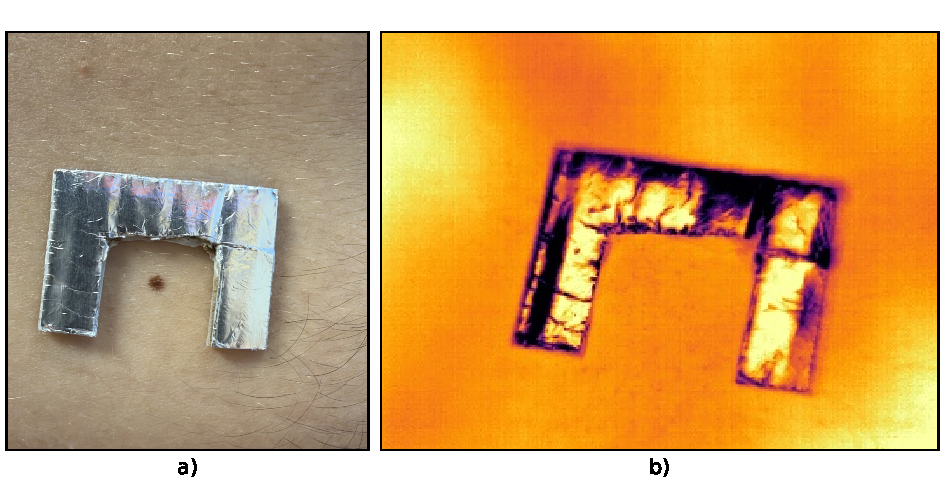
\includegraphics[width=\textwidth]{rysunki/para_14_rgb_termowizja.pdf}
  \caption{Zmiana skórna z naklejonym znacznikiem $\Pi$: a)~zdjęcie wykonane telefonem, b)~obraz termowizyjny 320~$\times$~240 pikseli. Znamię, widoczne na zdjęciu między ramionami znacznika, nie jest widoczne na termogramie. Źródło: opracowanie własne}
  \label{fig:para-wstep}
\end{figure}

Dodatkowym problemem jest weryfikacja wyniku. Nawet poprawnie wyglądające nałożenie obrazów nie gwarantuje, że obszar wyznaczony na zdjęciu odpowiada temu samemu fragmentowi skóry na termogramie. Ręczne oznaczanie punktów kontrolnych w każdej parze obrazów jest pracochłonne, dlatego pożądane jest rozwiązanie, które ocenia zgodność wyznaczenia obszaru automatycznie. Powyższe obserwacje stanowią motywację do podjęcia niniejszej pracy.

\section{Cel i zakres pracy}
\label{sec:cel}

Celem pracy jest opracowanie, implementacja oraz ocena systemu informatycznego umożliwiającego rejestrację i wspólną analizę obrazów dermatologicznych pochodzących z dwóch modalności: zdjęcia RGB wykonanego telefonem oraz obrazu termowizyjnego. System sprowadza oba obrazy do wspólnej przestrzeni odniesienia, przenosi obszar zainteresowania (ang.~\textit{region of interest}, ROI) między modalnościami i wyznacza jego parametry ilościowe. Zgodność wyznaczenia tego samego obszaru w obu modalnościach system weryfikuje, porównując maski segmentacji uzyskane modelami dedykowanymi każdej modalności, a wynikiem jest raport zawierający miary zgodności masek.
% TODO: porównać brzmienie celu z kartą tematu pracy (moja PG).

Aby osiągnąć ten cel, zrealizowano następujące zadania:
\begin{enumerate}
  \item przegląd literatury dotyczącej rejestracji obrazów wielomodalnych, segmentacji obrazów medycznych oraz miar oceny obu procesów;
  \item analizę wymagań i projekt systemu, obejmujący przypadki użycia, architekturę, diagram klas, bazę danych SQLite oraz interfejs użytkownika;
  \item zaprojektowanie znacznika referencyjnego w kształcie litery $\Pi$ (35~$\times$~26~mm, szerokość paska 9~mm, otwór 17~$\times$~17~mm), widocznego w obu modalnościach;
  \item zebranie własnego zbioru danych: 94 par zdjęcie--termogram przedstawiających 34 znamiona, wraz z ręcznymi adnotacjami wykonanymi w programie CVAT;
  \item implementację modułu rejestracji opartego na automatycznej detekcji znacznika i maksymalizacji rozszerzonego współczynnika korelacji (ECC);
  \item przygotowanie modeli segmentacji dla obu modalności: modelu PanDerm z dekoderem UperNet do segmentacji znamienia na zdjęciu oraz sieci U-Net do segmentacji znacznika na obrazie termowizyjnym;
  \item implementację przeniesienia ROI, pomiarów w milimetrach, miar zgodności masek oraz zapisu współrzędnych i surowej intensywności pikseli obrazu termowizyjnego w obszarze znamienia;
  \item implementację aplikacji z interfejsem graficznym, przetwarzania wsadowego i raportowania wyników;
  \item weryfikację systemu, obejmującą ocenę dokładności rejestracji, zgodności masek między modalnościami oraz jakości segmentacji;
  \item przygotowanie dokumentacji technicznej i instrukcji użytkownika.
\end{enumerate}

Zakres pracy nie obejmuje diagnostyki ani klasyfikacji zmian skórnych -- system nie stanowi narzędzia diagnostycznego. System zapisuje surowe intensywności pikseli obrazu termowizyjnego w obszarze znamienia, ale nie przelicza ich na temperaturę ani ich nie interpretuje; termografia dynamiczna stanowi jedynie kontekst rozważań.
Ponieważ znamię nie jest widoczne na termogramie, obszarem porównywanym między modalnościami jest otwór znacznika referencyjnego, w którym znajduje się znamię. Badania przeprowadzono na danych zebranych jednym zestawem urządzeń.

Wkład własny autora obejmuje projekt znacznika, zebranie i opisanie zbioru danych, metodę rejestracji opartą na maskach znacznika, douczenie i trening modeli segmentacji, badania weryfikacyjne oraz implementację aplikacji i bazy danych. W pracy wykorzystano gotowy koder modelu PanDerm udostępniony przez jego autorów~\cite{yan2025panderm} oraz biblioteki programistyczne wymienione w rozdziale~\ref{chap:projekt}.

\section{Struktura pracy}
\label{sec:struktura}

Praca składa się z siedmiu rozdziałów oraz dwóch dodatków. W rozdziale~\ref{chap:stan-wiedzy} przedstawiono przegląd literatury dotyczącej obrazowania zmian skórnych, rejestracji obrazów wielomodalnych, segmentacji oraz miar oceny. Rozdział~\ref{chap:analiza} zawiera analizę projektową: założenia, wymagania, przypadki użycia i architekturę systemu. W rozdziale~\ref{chap:projekt} opisano projekt systemu, w tym dobór technologii, projekt znacznika referencyjnego, bazy danych, diagram klas i interfejs użytkownika. Rozdział~\ref{chap:implementacja} przedstawia implementację poszczególnych modułów, a rozdział~\ref{chap:testy} -- wyniki badań weryfikacyjnych. Pracę zamyka podsumowanie wraz z kierunkami dalszych prac. Dodatek~A zawiera instrukcję użytkownika, a Dodatek~B -- dokumentację techniczną.

% =====================================================================
% Rozdział 2 – Analiza stanu wiedzy (WZÓR, ok. 7–8 stron z rysunkami)
% Styl bezosobowy. Wszystkie fakty pochodzą z kart w praca/materialy/03_streszczenia_artykulow.md.
% Rysunki z artykułów: materialy/rysunki_z_artykulow/ (ścieżki względem folderu praca/).
% Domyślnie włączone: 4 rysunki (Zitová, Oniga, U-Net, Taha) i 2 tabele. Rysunki Hermana i Hana są
% zakomentowane (OPCJA). Jeśli rozdział przekroczy 8 stron: usuń rys. Zitovej (fig:etapy-rejestracji),
% potem tabelę tab:panderm (liczby zostaw w tekście).
% Bez osobnych źródeł (decyzje 26.10): informację wzajemną cytuje się przez zitova2003/correlation-ratio (wariant Mattesa tylko jako metryka SimpleITK, rozdz. 6);
% nazwy GrabCut nie podaje się (,,segmentacja interaktywna z OpenCV''); ViT tylko jako koder PanDerm (yan2025panderm); analizy Blanda--Altmana nie opisuje się.
% =====================================================================

\chapter{Analiza stanu wiedzy}
\label{chap:stan-wiedzy}

W rozdziale omówiono kolejno: obrazowanie zmian skórnych w świetle widzialnym i w podczerwieni, metody rejestracji obrazów wielomodalnych, segmentację obrazów medycznych oraz miary oceny rejestracji i segmentacji. Rozdział zamyka zestawienie prac najbliższych tematowi i wskazanie luki, którą wypełnia niniejsza praca.

% ---------------------------------------------------------------------
\section{Obrazowanie zmian skórnych}
\label{sec:obrazowanie}

Podstawą oceny zmian barwnikowych jest obraz w świetle widzialnym. Dermatoskopia ogranicza odbicie światła od powierzchni skóry i uwidacznia struktury niewidoczne gołym okiem, a komputerowa analiza obrazów dermatoskopowych obejmuje segmentację zmiany, ekstrakcję cech i klasyfikację~\cite{dermoscopy}. Segmentacja jest pierwszym, a zarazem trudnym etapem tej analizy: utrudniają ją zmienność kształtu, rozmiaru i barwy zmian, włosy, naczynia oraz niejednolite warunki akwizycji~\cite{dermoscopy}. Celebi i in.~\cite{dermoscopy} zwracają uwagę, że metody sztucznej inteligencji można stosować także do zwykłych zdjęć wykonywanych z bliska, które dobrze oddają teksturę powierzchni skóry.

Termografia rejestruje promieniowanie podczerwone emitowane przez skórę. Emisyjność skóry wynosi 0,96--0,98, a maksimum jej emisji przypada na zakres 9--12~µm~\cite{infared-thermal-imaging}. Termogram przedstawia wyłącznie rozkład temperatury powierzchni, a wiarygodność pomiaru zależy od standaryzacji badania, w tym od powtarzalnego wyznaczania obszaru zainteresowania -- jego kształt, rozmiar i położenie wpływają na wynik diagnostyczny~\cite{infared-thermal-imaging}.

W termografii statycznej obraz rejestruje się bez stymulacji, a w dynamicznej -- po bodźcu termicznym, chemicznym lub mechanicznym~\cite{magalhaes2019}. Herman i Pirtini Cetingul~\cite{visualization-detection-cancer} chłodzą zmianę wraz z otoczeniem o średnicy 50~mm strumieniem zimnego powietrza przez 1~min, a następnie co 2~s rejestrują powrót temperatury trwający 3--4~min. Ponieważ bez schłodzenia zmiana jest niewidoczna na termogramie, wokół niej przykleja się kwadratowy znacznik, którego narożniki służą do rejestracji zdjęcia z sekwencją obrazów w podczerwieni. Magalhaes i in.~\cite{magalhaes2019} porównali termografię statyczną i dynamiczną dla 46 zmian (16 czerniaków i 30 znamion) zarejestrowanych kamerą o rozdzielczości 320~$\times$~240 pikseli; najlepszy klasyfikator, wykorzystujący cechy statyczne, osiągnął dokładność 84,2\% przy czułości 91,3\%. Obszar analizy wyznaczano tam ręcznie jako okno 40~$\times$~40 pikseli umieszczane przez użytkownika.

% OPCJA (rys. z pracy Hermana – znacznik na skórze i termogram po schłodzeniu): odkomentuj, jeśli zmieści się w limicie 8 stron.
% \begin{figure}[htbp]
%   \centering
%   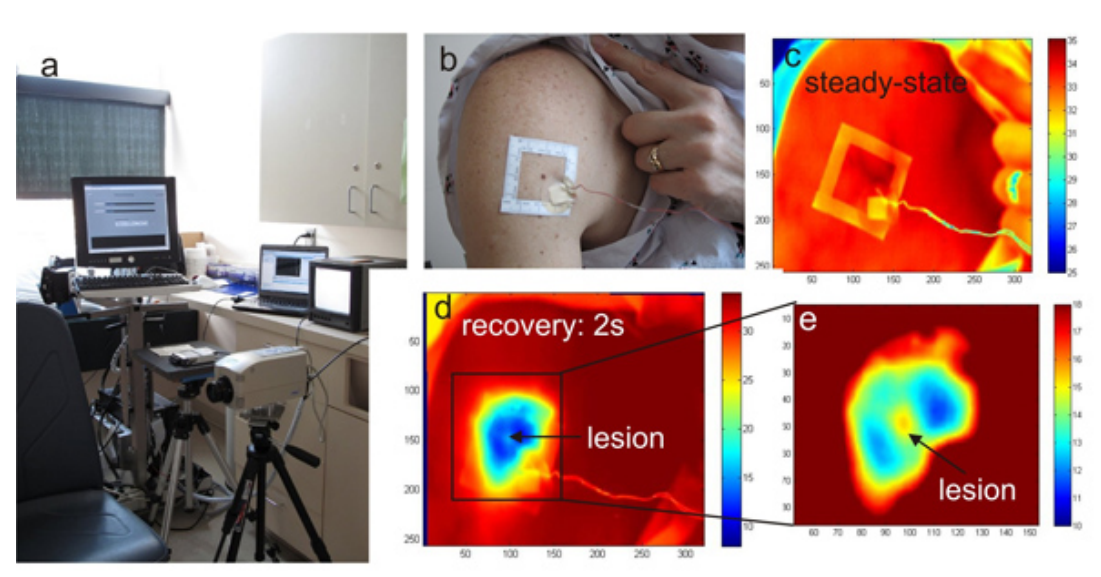
\includegraphics[width=\textwidth]{materialy/rysunki_z_artykulow/R01_herman2011_fig1.png}
%   \caption{Stanowisko do termografii dynamicznej oraz zmiana barwnikowa ze znacznikiem: a)~system obrazowania, b)~zdjęcie skóry z naklejoną ramką, c)~obraz w podczerwieni w temperaturze otoczenia, d)~ten sam obszar po schłodzeniu, e)~powiększenie zmiany. Źródło:~\cite{visualization-detection-cancer}}
%   \label{fig:herman}
% \end{figure}

Obraz widzialny i obraz podczerwony są komplementarne: pierwszy ma bogatą teksturę, lecz zależy od oświetlenia, drugi niesie informację termiczną niezależną od oświetlenia, ale ubogą w szczegóły~\cite{deep-learning}. Łączenie obu modalności wymaga jednak ich wcześniejszej rejestracji, omówionej w kolejnym podrozdziale.

% ---------------------------------------------------------------------
\section{Rejestracja obrazów wielomodalnych}
\label{sec:rejestracja}

\subsection{Modele transformacji i miary podobieństwa}
\label{sec:modele-transformacji}

Rejestracja obrazów to proces nakładania dwóch lub więcej obrazów tej samej sceny wykonanych w różnym czasie, z różnych punktów widzenia lub różnymi sensorami, czyli geometryczne dopasowanie obrazu rejestrowanego do obrazu referencyjnego~\cite{zitova2003}. Zitová i Flusser~\cite{zitova2003} opisują ją czterema etapami: detekcją cech, dopasowaniem cech, estymacją modelu transformacji oraz transformacją i przepróbkowaniem obrazu (rys.~\ref{fig:etapy-rejestracji}). Metody dzieli się na obszarowe (ang.~\textit{area-based}), porównujące bezpośrednio intensywności, oraz oparte na cechach (ang.~\textit{feature-based}). Metody obszarowe wymagają, aby intensywności obu obrazów były identyczne albo przynajmniej statystycznie zależne, natomiast metody oparte na cechach nadają się do rejestracji obrazów z różnych sensorów~\cite{zitova2003}.

\begin{figure}[htbp]
  \centering
  \includegraphics[width=0.6\textwidth]{materialy/rysunki_z_artykulow/R03_zitova2003_fig1.png}
  \caption{Etapy rejestracji obrazów: detekcja cech (u góry), dopasowanie cech (w środku), estymacja modelu transformacji (na dole po lewej) oraz przepróbkowanie obrazu (na dole po prawej). Źródło:~\cite{zitova2003}}
  \label{fig:etapy-rejestracji}
\end{figure}

Wybór modelu transformacji określa, jakie zniekształcenia mogą zostać skompensowane. Model podobieństwa (obrót, przesunięcie, jednolita skala) wyznaczają dwa punkty kontrolne, model afiniczny -- trzy niewspółliniowe punkty; zachowuje on proste i równoległość. Przekształcenie perspektywiczne (homografia) dokładnie opisuje płaską scenę fotografowaną kamerą, której oś optyczna nie jest prostopadła do sceny, i wymaga czterech punktów kontrolnych~\cite{zitova2003}. W pracy~\cite{gonzalezperez2021} homografia, mimo największej liczby stopni swobody, najsłabiej przenosiła się na obrazy wykonane w innej odległości niż obrazy, na których ją wyznaczono. Oniga i in.~\cite{oniga2026} uzasadniają z kolei wybór homografii tym, że niewielki fragment skóry ze sztywnym znacznikiem jest lokalnie quasi-płaski.

W metodach obszarowych transformację wyznacza się przez optymalizację miary podobieństwa. Evangelidis i Psarakis~\cite{evangelidis2008} zaproponowali kryterium rozszerzonego współczynnika korelacji (ang.~\textit{enhanced correlation coefficient}, ECC), które -- dzięki odjęciu średniej i normalizacji wektorów intensywności -- jest niezmiennicze względem zmian jasności i kontrastu. Kryterium jest nieliniowe względem parametrów, dlatego autorzy zaproponowali iteracyjne schematy optymalizacji z rozwiązaniem w postaci zamkniętej w każdej iteracji; w eksperymentach symulacyjnych osiągały one mniejszy błąd i częstszą zbieżność niż odpowiadające im warianty algorytmu Lucasa--Kanade~\cite{evangelidis2008}. Jak wszystkie metody gradientowe, ECC wymaga jednak dobrego punktu startowego i ma trudności w obszarach jednorodnych oraz przy dużych przesunięciach~\cite{evangelidis2008}. W rejestracji wielomodalnej stosuje się miary statystyczne, przede wszystkim informację wzajemną~\cite{zitova2003}, która nie zakłada postaci zależności między intensywnościami; Roche i in.~\cite{correlation-ratio} pokazali jednak na przykładzie syntetycznym, że może ona mieć wiele równoważnych maksimów.

W niniejszej pracy miarę podobieństwa oblicza się nie na surowych obrazach, lecz na maskach znacznika wyodrębnionych w obu modalnościach, co sprowadza problem wielomodalny do jednomodalnego i umożliwia zastosowanie kryterium ECC.

\subsection{Rejestracja obrazów widzialnych i termowizyjnych}
\label{sec:rgb-ir}

Rejestrację obrazów widzialnych i termowizyjnych utrudnia odmienny mechanizm ich powstawania: jasność w podczerwieni zależy od temperatury i emisyjności obiektów, a w świetle widzialnym -- od światła odbitego, więc intensywności nie są bezpośrednio powiązane~\cite{visible-and-infared}. Han i in.~\cite{visible-and-infared} wykazali, że punkty charakterystyczne SURF i Harrisa wykrywane w obu modalnościach w dużej mierze się nie pokrywają. Zaproponowana przez nich metoda wykorzystuje proste wyprowadzone z krawędzi obiektów, przez co wymaga struktur typowych dla otoczenia zbudowanego przez człowieka i nie przenosi się na obrazy skóry.

% OPCJA (rys. z pracy Hana – punkty SURF/Harris): odkomentuj, jeśli zmieści się w limicie 8 stron.
% \begin{figure}[htbp]
%   \centering
%   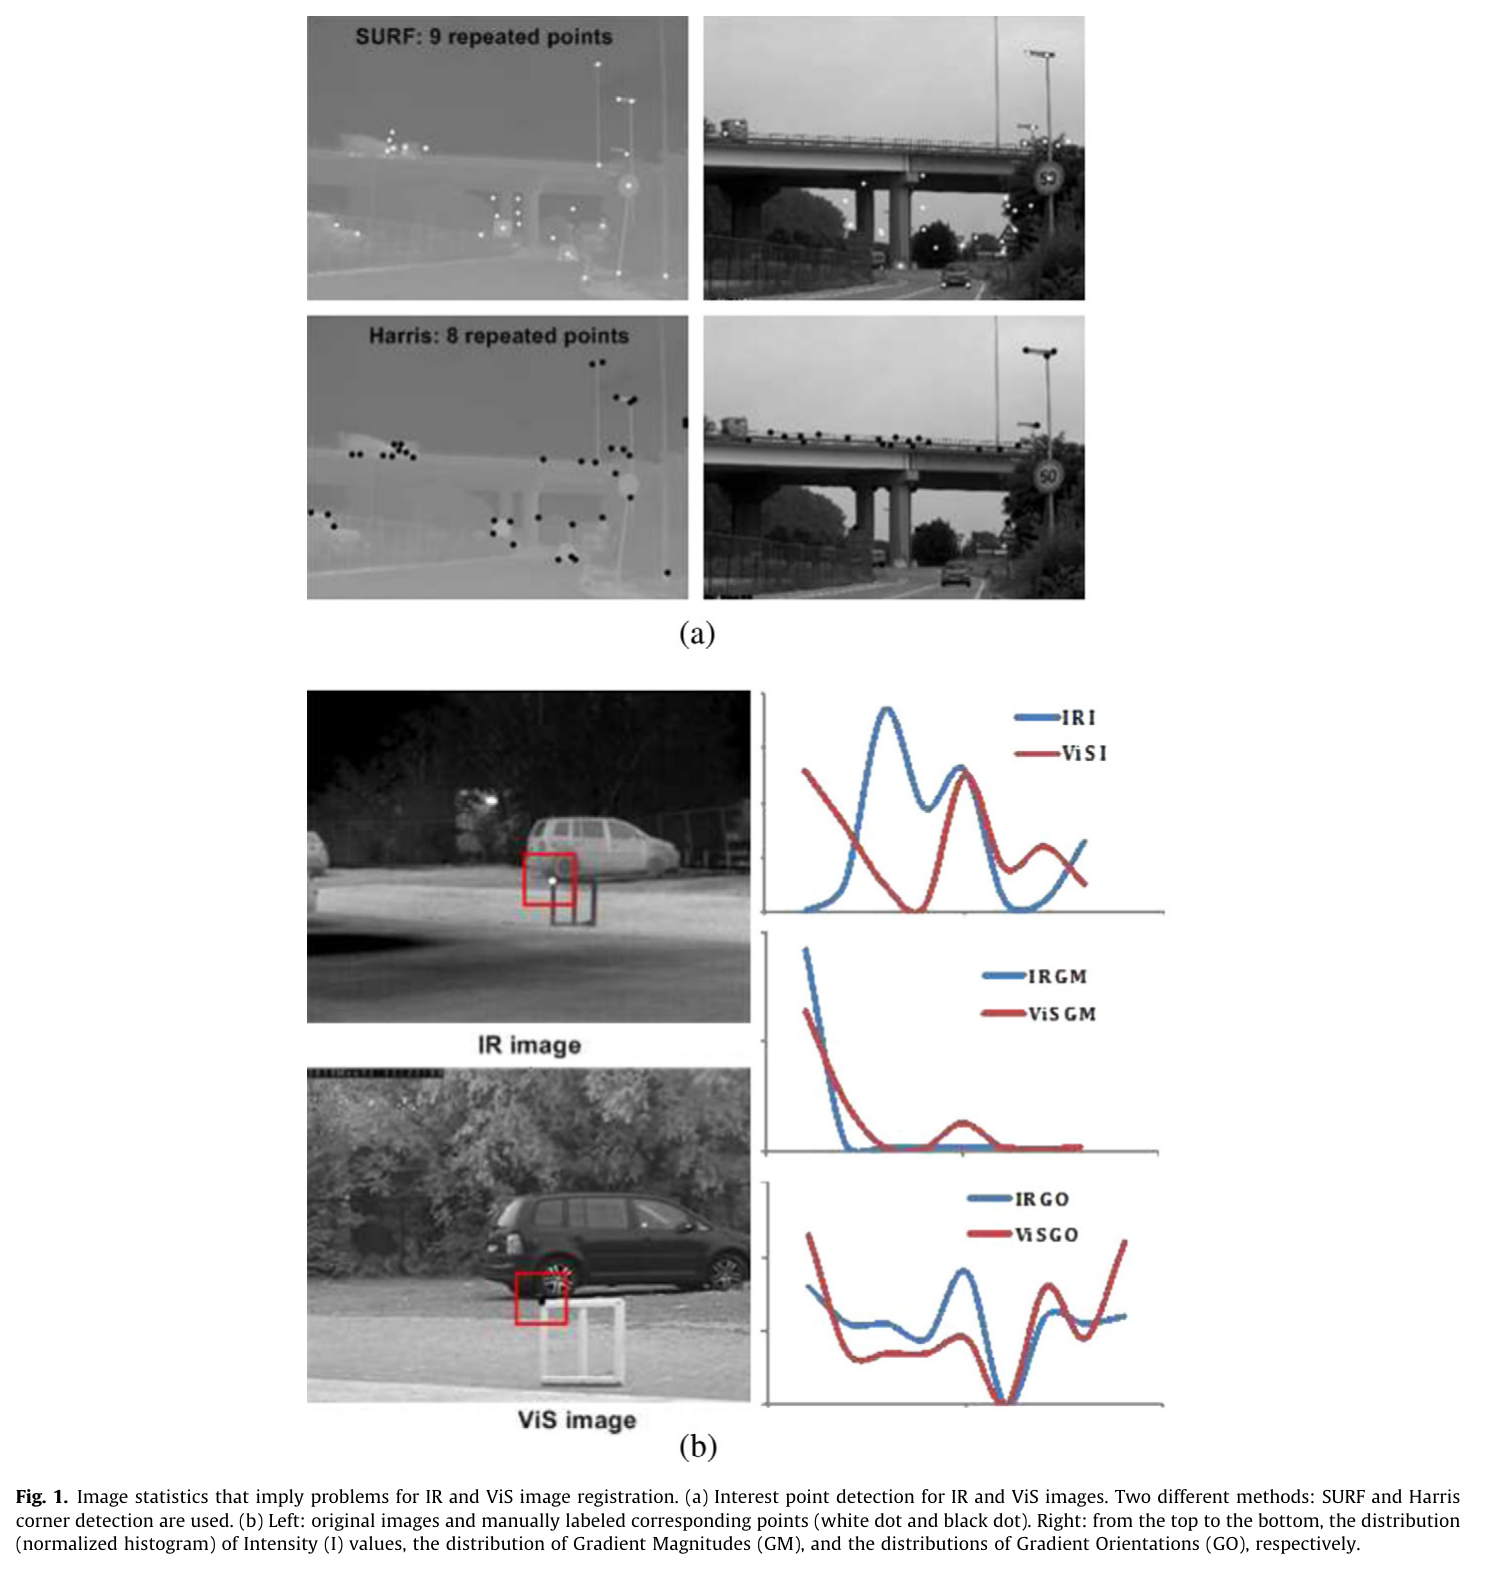
\includegraphics[width=0.6\textwidth]{materialy/rysunki_z_artykulow/R08_han2013_fig1.png}
%   \caption{Problemy rejestracji obrazów podczerwonych i widzialnych: a)~punkty charakterystyczne SURF i Harrisa wykryte w obu modalnościach, b)~rozkłady intensywności i gradientów w odpowiadających sobie fragmentach. Źródło:~\cite{visible-and-infared}}
%   \label{fig:han}
% \end{figure}

W zastosowaniach medycznych korespondencję zapewnia się zwykle obiektem widocznym w obu modalnościach. González-Pérez i in.~\cite{gonzalezperez2021} porównali cztery metody rejestracji obrazów stopy w systemie z kamerami połączonymi na sztywno; punkty kalibracyjne dawała szachownica umieszczona przed schłodzoną płytą aluminiową, kontrastującą termicznie z otoczeniem. Metoda afiniczna optymalizowana na binarnych maskach stóp uzyskała w płaszczyźnie ostrości kamer (800~mm) współczynnik Dice'a 0,982, przy czym na surowych obrazach różnych widm optymalizacja ta nie zbiegała poprawnie~\cite{gonzalezperez2021}. Maurya i in.~\cite{non-contact-breathing-monitoring} wyznaczają punkty kontrolne na ramie kalibracyjnej wyciętej z materiału słabo przewodzącego ciepło, a transformację doprecyzowują cechami opartymi na zgodności fazy, uzyskując średni błąd rejestracji 1,817 piksela dla 50 par obrazów. Obszar zainteresowania wyznaczają i śledzą w obrazie RGB, a następnie przenoszą go na obraz termowizyjny, ubogi w teksturę~\cite{non-contact-breathing-monitoring}.

Najbliższe tematowi niniejszej pracy jest rozwiązanie Onigi i in.~\cite{oniga2026}, którzy rejestrują obrazy zmian skórnych w świetle widzialnym, bliskiej podczerwieni i termowizji z użyciem kwadratowego znacznika umieszczonego na skórze wokół zmiany (rys.~\ref{fig:oniga}). Znacznik lokalizuje detektor YOLOv8n, a homografię wyznacza się z punktów kluczowych przewidywanych przez sieć neuronową. Autorzy zauważają, że w obrazie termowizyjnym znacznik bywa słabiej widoczny i ma zaokrąglone narożniki, a zmiana skórna często nie jest widoczna. Wyniki oceniano wyłącznie miarami podobieństwa obrazów (SSIM, MI, NMI), bez miar geometrycznych~\cite{oniga2026}.

\begin{figure}[htbp]
  \centering
  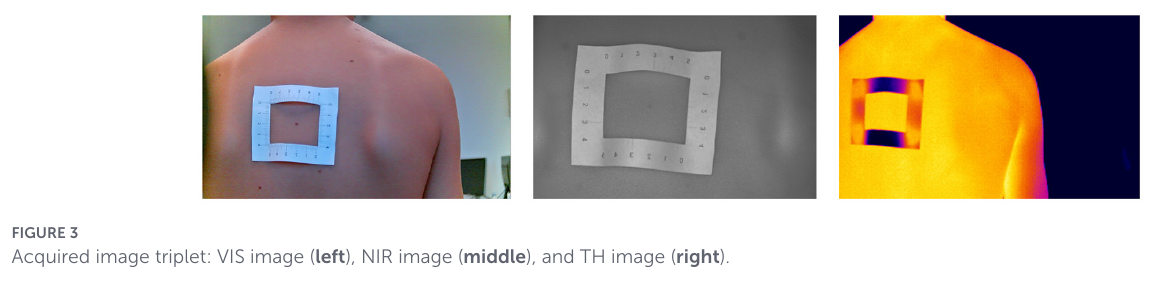
\includegraphics[width=0.8\textwidth]{materialy/rysunki_z_artykulow/R07_oniga2026_fig3.png}
  \caption{Kwadratowy znacznik referencyjny na skórze w obrazie widzialnym (po lewej), w bliskiej podczerwieni (w środku) i w obrazie termowizyjnym (po prawej). Źródło:~\cite{oniga2026}}
  \label{fig:oniga}
\end{figure}

\subsection{Metody oparte na uczeniu głębokim}
\label{sec:rejestracja-dl}

Przegląd Chena i in.~\cite{deep-learning-in-registration}, obejmujący 77 prac, dzieli metody głębokiej rejestracji obrazów medycznych na trzy grupy: sieci pełniące rolę miary podobieństwa, sieci bezpośrednio wyznaczające parametry transformacji (w wariantach nadzorowanym, słabo nadzorowanym i nienadzorowanym) oraz pozostałe zastosowania. Przykładem podejścia słabo nadzorowanego jest praca Hu i in.~\cite{neural-networks}, w której sieć konwolucyjna przewiduje pole przemieszczeń między obrazami MR i TRUS prostaty; etykiety anatomiczne są potrzebne wyłącznie podczas uczenia, a w fazie wnioskowania wystarcza para obrazów. Autorzy uzyskali medianę błędu w punktach docelowych 3,6~mm na 108 parach obrazów, podczas gdy klasyczna rejestracja oparta na miarach intensywności zawiodła na tych danych~\cite{neural-networks}. Metody głębokie wymagają jednak licznych danych uczących, a publicznie dostępnych zbiorów wielomodalnych jest niewiele~\cite{deep-learning-in-registration}. Dla pary telefon--kamera termowizyjna takich danych nie ma, dlatego w niniejszej pracy zastosowano rejestrację klasyczną opartą na znaczniku.

\subsection{Fuzja i wizualizacja nałożenia}
\label{sec:fuzja}

Zhang i Demiris~\cite{deep-learning} wyróżniają fuzję obrazów widzialnych i podczerwonych na poziomie pikseli, cech i decyzji; w literaturze termin ten odnosi się zwykle do poziomu pikseli, na którym powstaje jeden obraz wynikowy. Fuzja pikselowa wymaga dokładnej rejestracji, a autorzy uznają wyrównanie obrazów widzialnych i podczerwonych za problem otwarty, wskazując wspólne uczenie rejestracji i fuzji jako kierunek badań~\cite{deep-learning}. W niniejszej pracy nałożenie obrazów pełni funkcję wizualizacji wyniku rejestracji, a wspólna analiza odbywa się przez przeniesienie obszaru zainteresowania, podobnie jak w~\cite{non-contact-breathing-monitoring}.

% ---------------------------------------------------------------------
\section{Segmentacja obrazów medycznych}
\label{sec:segmentacja}

\subsection{Metody klasyczne}
\label{sec:segmentacja-klasyczna}

Przed upowszechnieniem uczenia głębokiego segmentację zmian skórnych realizowano m.in. progowaniem adaptacyjnym, konturami aktywnymi, rozrostem obszaru i klasteryzacją (za:~\cite{mirikharaji2023}). Metody te opierają się na cechach projektowanych ręcznie, co ogranicza ich skuteczność na dużych i zróżnicowanych zbiorach danych~\cite{mirikharaji2023}. W niniejszej pracy metody klasyczne wykorzystano do detekcji znacznika referencyjnego, który ma znany kształt i wyraźnie kontrastuje ze skórą.

\subsection{Sieć U-Net i architektury koder--dekoder}
\label{sec:unet}

Ronneberger i in.~\cite{ronneberger2015} zaproponowali sieć U-Net do segmentacji obrazów biomedycznych przy bardzo małej liczbie oznaczonych obrazów. Ścieżka kurcząca (koder) gromadzi kontekst, symetryczna ścieżka rozszerzająca (dekoder) zapewnia dokładną lokalizację, a połączenia skrótowe przekazują cechy wysokiej rozdzielczości z kodera do dekodera (rys.~\ref{fig:unet}). Kluczowym elementem uczenia była intensywna augmentacja, zwłaszcza losowe deformacje sprężyste; sieć uczona na 30 obrazach z mikroskopii elektronowej zajęła pierwsze miejsce w rankingu wyzwania ISBI według błędu deformacji~\cite{ronneberger2015}. Według przeglądu~\cite{mirikharaji2023}, obejmującego 177 prac o segmentacji zmian skórnych, połączenia skrótowe stosuje 112 z nich, a najczęstszymi funkcjami straty są entropia krzyżowa i strata Dice.

\begin{figure}[htbp]
  \centering
  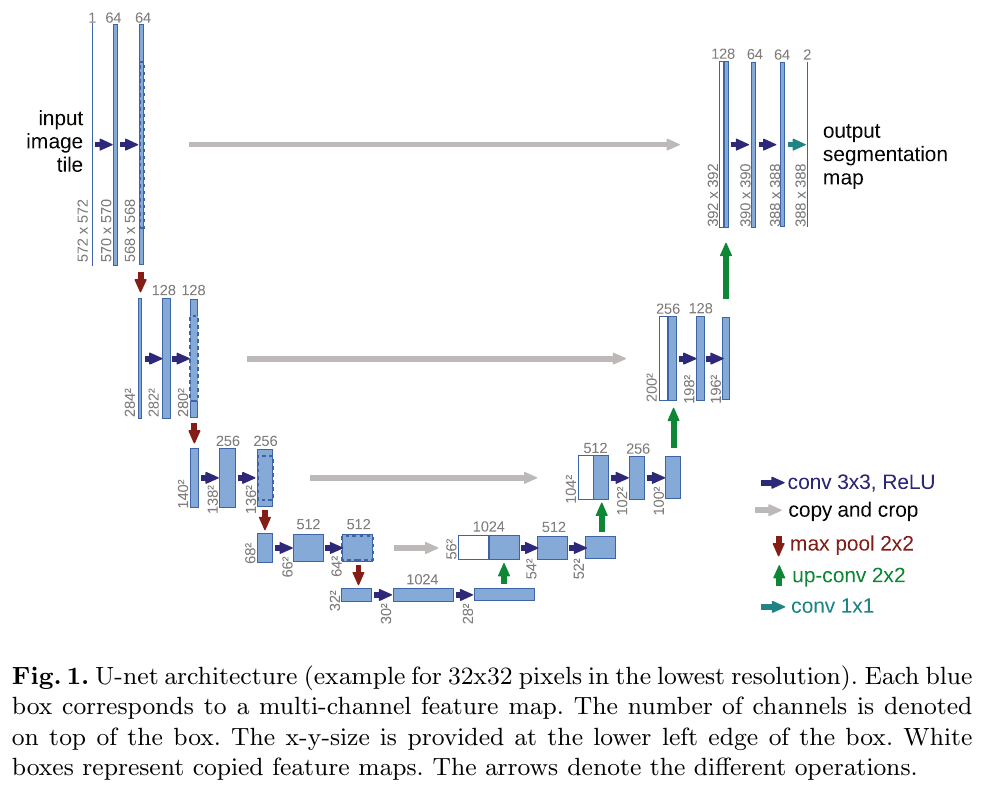
\includegraphics[width=0.6\textwidth]{materialy/rysunki_z_artykulow/R13_ronneberger2015_fig1.png}
  \caption{Architektura sieci U-Net. Prostokąty oznaczają mapy cech (nad nimi liczba kanałów), strzałki -- operacje. Źródło:~\cite{ronneberger2015}}
  \label{fig:unet}
\end{figure}

Dekoder UperNet~\cite{xiao2018upernet} łączy piramidę cech (ang.~\textit{Feature Pyramid Network}, FPN) z modułem łączenia piramidalnego (ang.~\textit{Pyramid Pooling Module}, PPM) dołączonym do najgłębszej warstwy kodera. Moduł PPM wnosi kontekst globalny, a fuzja map cech ze wszystkich poziomów piramidy poprawia wynik segmentacji; w oryginalnej pracy na zbiorze ADE20K konfiguracja FPN~+~PPM z fuzją osiągnęła mIoU 41,22\%~\cite{xiao2018upernet}.

\subsection{Modele bazowe w dermatologii i zbiory danych}
\label{sec:modele-bazowe}

Model bazowy (ang.~\textit{foundation model}) to duża sieć wstępnie uczona samonadzorowanie na dużym, zróżnicowanym zbiorze danych, którą można douczyć do konkretnego zadania przy niewielkiej liczbie etykiet~\cite{yan2025panderm}. PanDerm~\cite{yan2025panderm} to model bazowy dla dermatologii z koderem typu ViT-Large, uczony na 2~149~706 obrazach z 11 źródeł w czterech modalnościach: fotografii całego ciała, dermatopatologii, zdjęciach klinicznych (460~328 obrazów) i obrazach dermatoskopowych. W zadaniu segmentacji, z dekoderem UperNet, model uzyskał Dice 0,910 na zbiorze ISIC 2018 i 0,949 na HAM10000, przewyższając modele porównawcze (tab.~\ref{tab:panderm}); przy 5\% danych uczących dorównywał najlepszemu z pozostałych modeli uczonych na pełnym zbiorze~\cite{yan2025panderm}. Segmentację oceniono jednak wyłącznie na obrazach dermatoskopowych.

\begin{table}[htbp]
  \centering
  \caption{Wyniki segmentacji zmian skórnych modelu PanDerm i modeli porównawczych (DSC -- współczynnik Dice'a, JAC -- indeks Jaccarda). Opracowanie własne na podstawie~\cite{yan2025panderm}}
  \label{tab:panderm}
  \begin{tabular}{lcccc}
    \toprule
    Model & \multicolumn{2}{c}{ISIC 2018} & \multicolumn{2}{c}{HAM10000} \\
     & DSC & JAC & DSC & JAC \\
    \midrule
    SL-ImageNet & 0,876 & 0,807 & 0,927 & 0,875 \\
    autoSMIM    & 0,848 & 0,769 & 0,920 & 0,865 \\
    BATFormer   & 0,884 & 0,815 & 0,937 & 0,891 \\
    PanDerm     & \textbf{0,910} & \textbf{0,846} & \textbf{0,949} & \textbf{0,910} \\
    \bottomrule
  \end{tabular}
\end{table}

Najczęściej wykorzystywanymi zbiorami do segmentacji zmian skórnych są zbiory wyzwań ISIC, użyte w 168 ze 177 prac objętych przeglądem~\cite{mirikharaji2023}. Zbiór zadania segmentacji ISIC 2018 obejmuje 3694 obrazy dermatoskopowe z oficjalnym podziałem na 2594 obrazy uczące, 100 walidacyjnych i 1000 testowych~\cite{codella2019,mirikharaji2023}. Zbiór HAM10000~\cite{tschandl2018} zawiera 10~015 obrazów dermatoskopowych z dwóch ośrodków, zebranych w ciągu 20 lat i przypisanych do siedmiu klas diagnostycznych. W wyzwaniu ISIC 2018 wprowadzono progowany indeks Jaccarda, w którym wynik dla obrazu poniżej 0,65 zastępuje się zerem, traktując segmentację jako porażkę; próg wyznaczono na podstawie zgodności trzech ekspertów, których średni indeks Jaccarda wynosił 0,786~\cite{codella2019}. Problem segmentacji pozostaje otwarty -- najlepsze zgłoszenie uzyskało progowany indeks Jaccarda 0,802, a mimo średnich wartości indeksu Jaccarda powyżej 0,8 większość metod zawodziła na ponad 10\% obrazów, najczęściej w przypadku rogowacenia łojotokowego~\cite{codella2019}. Jednocześnie liczba zdjęć klinicznych z maskami segmentacji od lat pozostaje niewielka w porównaniu z obrazami dermatoskopowymi~\cite{mirikharaji2023}, dlatego modele uczone na dermoskopii stosowane do zdjęć z telefonu pracują w warunkach przesunięcia dziedziny (ang.~\textit{domain shift}).

\subsection{Segmentacja obrazów termowizyjnych}
\label{sec:segmentacja-termo}

Ponieważ znamię bez schłodzenia skóry nie jest widoczne na termogramie, w pracach dotyczących termografii zmian skórnych obrys wyznacza się na obrazie widzialnym i przenosi na obraz w podczerwieni~\cite{visualization-detection-cancer} albo obszar analizy ustawia się ręcznie~\cite{magalhaes2019}. W termowizji można natomiast wyznaczyć obiekt referencyjny o odmiennych własnościach termicznych -- znacznik~\cite{oniga2026}. Z tego względu w niniejszej pracy model segmentacji dedykowany termowizji wyznacza maskę znacznika, a nie znamienia.

% ---------------------------------------------------------------------
\section{Miary oceny rejestracji i segmentacji}
\label{sec:miary}

Fitzpatrick i in.~\cite{fitzpatrick1998} rozróżniają trzy rodzaje błędów rejestracji opartej na punktach: błąd lokalizacji znacznika (ang.~\textit{fiducial localization error}, FLE), błąd dopasowania znaczników po rejestracji (ang.~\textit{fiducial registration error}, FRE) oraz błąd w punkcie docelowym (ang.~\textit{target registration error}, TRE), czyli odległość między odpowiadającymi sobie punktami po rejestracji. Autorzy wykazali, że FRE nie zależy od konfiguracji znaczników i jest zawodnym wskaźnikiem dokładności, natomiast TRE rośnie wraz z odległością celu od środka konfiguracji~\cite{fitzpatrick1998}. Dokładność rejestracji należy więc oceniać na punktach, które nie uczestniczyły w wyznaczaniu transformacji; zdaniem Zitovej i Flussera~\cite{zitova2003} bez oceny ilościowej żadna metoda rejestracji nie może zostać przyjęta do praktycznego zastosowania.

Taha i Hanbury~\cite{taha2015} zestawili 20 miar oceny segmentacji w sześciu kategoriach, m.in. miary pokrycia, objętościowe i odległościowe. Współczynnik Dice'a i indeks Jaccarda są ze sobą powiązane monotonicznie, dlatego dają ten sam ranking segmentacji. Miary pokrycia nie wykrywają błędów kształtu brzegu (rys.~\ref{fig:taha}) i nie są zalecane dla małych obiektów, a odległość Hausdorffa jest wrażliwa na punkty odstające, dlatego zastępuje się ją kwantylem odległości~\cite{taha2015}. Zgodnie z zaleceniami Metrics Reloaded~\cite{maierhein2024}, opracowanymi w procesie delfickim przez międzynarodowe konsorcjum ekspertów, w segmentacji semantycznej miarę pokrycia (DSC lub IoU) uzupełnia się miarą brzegową, np. 95.~percentylem odległości Hausdorffa (HD95) lub średnią symetryczną odległością powierzchni (ASSD). Te same zalecenia wskazują, że miary należy liczyć osobno dla każdego obrazu i agregować z uwzględnieniem hierarchii danych~\cite{maierhein2024}. Podobne podejście -- ocenę rejestracji przez zgodność masek po przeniesieniu -- zastosowano w pracy~\cite{gonzalezperez2021}.

\begin{figure}[htbp]
  \centering
  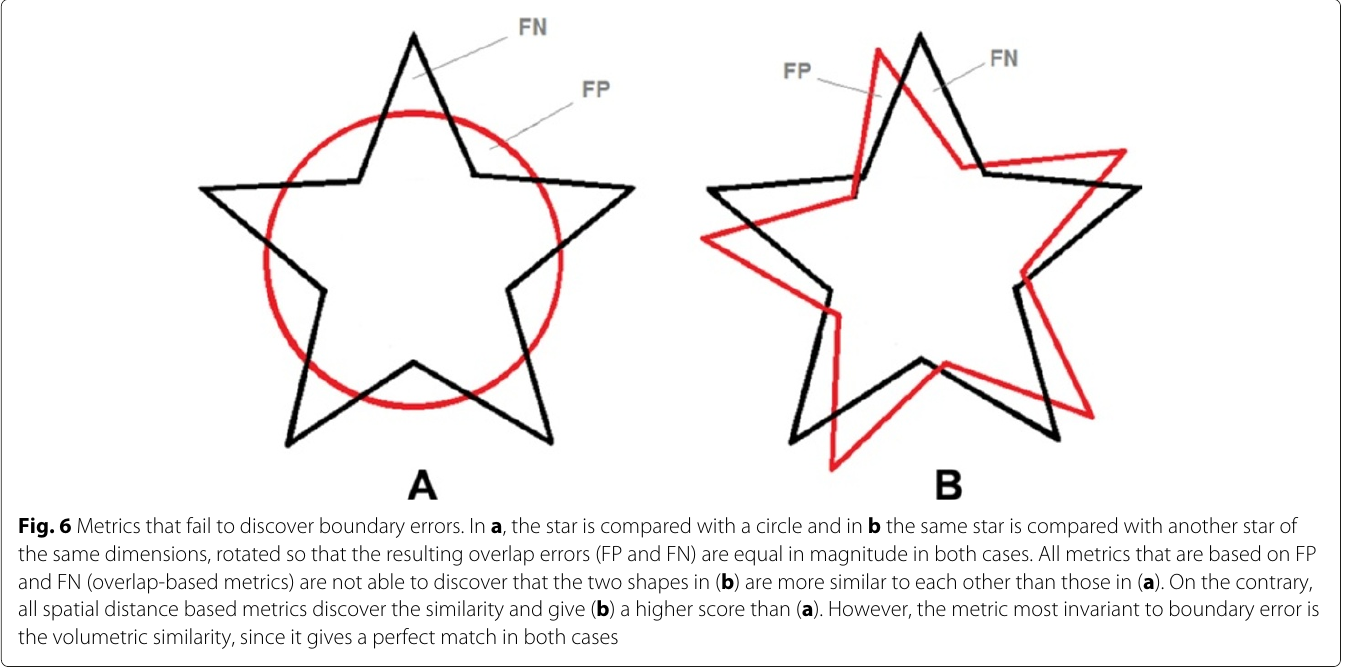
\includegraphics[width=0.65\textwidth]{materialy/rysunki_z_artykulow/R18_taha2015_fig6.png}
  \caption{Przykład, w którym miary pokrycia nie wykrywają błędu brzegu: w obu przypadkach liczby pikseli fałszywie dodatnich i fałszywie ujemnych są równe, mimo różnego podobieństwa kształtów. Źródło:~\cite{taha2015}}
  \label{fig:taha}
\end{figure}

W niniejszej pracy dokładność rejestracji oceniano błędem TRE wyznaczanym na narożnikach znacznika oznaczonych ręcznie, które nie uczestniczą w wyznaczaniu transformacji, a zgodność masek -- współczynnikiem Dice'a uzupełnionym miarami HD95 i ASSD wyrażonymi w milimetrach.

% ---------------------------------------------------------------------
\section{Podsumowanie i luka badawcza}
\label{sec:luka}

Zestawienie prac rejestrujących obraz widzialny z termowizyjnym przedstawiono w tabeli~\ref{tab:prace-rgb-ir}. We wszystkich rozwiązaniach przeznaczonych dla medycyny korespondencję między modalnościami zapewnia obiekt referencyjny, a obszar zainteresowania wyznacza się w obrazie widzialnym. Prace różnią się jednak sposobem oceny: stosowano błąd w pikselach, zgodność masek albo miary podobieństwa obrazów, a w żadnej z nich nie weryfikowano zgodności przeniesionego obszaru niezależnym modelem segmentacji drugiej modalności.

\begin{table}[htbp]
  \centering
  \caption{Prace rejestrujące obraz widzialny z obrazem termowizyjnym. Opracowanie własne na podstawie~\cite{visualization-detection-cancer,visible-and-infared,non-contact-breathing-monitoring,gonzalezperez2021,oniga2026}}
  \label{tab:prace-rgb-ir}
  \small
  \begin{tabularx}{\textwidth}{>{\raggedright\arraybackslash}p{2.4cm} >{\raggedright\arraybackslash}X >{\raggedright\arraybackslash}X >{\raggedright\arraybackslash}X}
    \toprule
    Praca & Zastosowanie & Źródło korespondencji & Ocena rejestracji \\
    \midrule
    Herman i Pirtini Cetingul~\cite{visualization-detection-cancer} & termografia dynamiczna zmian barwnikowych & narożniki kwadratowego znacznika na skórze & brak miar ilościowych \\
    Han i in.~\cite{visible-and-infared} & sceny zurbanizowane & proste z krawędzi obiektów, punkty Harrisa & błąd w pikselach \\
    Maurya i in.~\cite{non-contact-breathing-monitoring} & pomiar częstości oddechu & rama kalibracyjna, cechy zgodności fazy & TRE 1,817 piksela (50 par) \\
    González-Pérez i in.~\cite{gonzalezperez2021} & monitorowanie stopy cukrzycowej & szachownica z płytą aluminiową, maski stóp & Dice i Jaccard masek \\
    Oniga i in.~\cite{oniga2026} & zmiany skórne (VIS, NIR, TH) & kwadratowy znacznik, punkty z sieci neuronowej & SSIM, MI, NMI \\
    Niniejsza praca & zmiany skórne & kształt znacznika $\Pi$ (maski w obu modalnościach) & TRE w mm, zgodność masek z modelu segmentacji termowizji \\
    \bottomrule
  \end{tabularx}
\end{table}

Z przeglądu wynikają trzy wnioski dla projektu systemu. Po pierwsze, ze względu na brak wspólnych cech naturalnych i niewidoczność znamienia na termogramie korespondencję należy oprzeć na znaczniku widocznym w obu modalnościach. Po drugie, brak dużego zbioru par telefon--termogram przemawia za klasyczną rejestracją na maskach znacznika, a w segmentacji -- za douczaniem modelu bazowego i niewielkimi sieciami typu U-Net. Po trzecie, ocena powinna łączyć błąd w punktach docelowych z miarami pokrycia i miarami brzegowymi. W przeanalizowanej literaturze nie znaleziono systemu, który rejestruje zdjęcie z telefonu z termogramem na podstawie znacznika o znanym kształcie i weryfikuje zgodność przeniesionego obszaru modelem segmentacji dedykowanym drugiej modalności, bez potrzeby ręcznych adnotacji. Lukę tę wypełnia niniejsza praca.

% =====================================================================
% Rozdział 3 – Analiza projektowa (WZÓR, ok. 4 strony)
% Styl bezosobowy. Rysunki: rysunki/przypadki_uzycia.pdf, architektura_systemu.pdf,
% potok_przetwarzania.pdf (ścieżki względem folderu praca/).
% Wymaga pakietów: booktabs, tabularx.
% Przy braku miejsca (budżet ok. 4 s.): usuń tabelę tab:scenariusz albo przenieś rys. fig:potok na początek rozdz. 5.
% =====================================================================

\chapter{Analiza projektowa}
\label{chap:analiza}

W rozdziale przedstawiono założenia, przy których projektowano system, wymagania funkcjonalne i pozafunkcjonalne, przypadki użycia oraz architekturę systemu. Opisano tu, \emph{co} system ma realizować; sposób realizacji omówiono w rozdziale~\ref{chap:projekt}.

\section{Założenia i ograniczenia}
\label{sec:zalozenia}

System jest przeznaczony dla studentów i lekarzy współpracujących z Uniwersyteckim Centrum Klinicznym w Gdańsku. % TODO: potwierdzić grupę użytkowników z promotorką.
Przy jego projektowaniu przyjęto następujące założenia:
\begin{itemize}
  \item danymi wejściowymi są dwa obrazy tej samej zmiany: zdjęcie RGB wykonane telefonem (format JPG) oraz obraz termowizyjny o rozdzielczości 320~$\times$~240 pikseli, wyodrębniony z nagrania kamery termowizyjnej FLIR A320 z obiektywem 18~mm (format .SEQ);
  \item obrazy pochodzą z dwóch niezależnych urządzeń, niesprzężonych i nieskalibrowanych względem siebie, a każde zdjęcie wykonywane jest z innej odległości i pod innym kątem -- transformację między obrazami należy więc wyznaczać osobno dla każdej pary;
  \item na skórze wokół zmiany nakleja się znacznik referencyjny w kształcie litery $\Pi$, a znamię znajduje się między jego ramionami; przyjęto, że skóra w obrębie znacznika jest w przybliżeniu płaska, dzięki czemu zależność między obrazami opisuje przekształcenie afiniczne lub homografia;
  \item znamię nie jest widoczne na obrazie termowizyjnym, dlatego w tej modalności segmentuje się znacznik, a obszarem porównywanym między modalnościami jest otwór znacznika;
  \item system działa w pełni automatycznie; ręczne adnotacje wykonane w programie CVAT służą wyłącznie do oceny wyników;
  \item system działa lokalnie na komputerze z systemem Windows; model segmentacji znamienia wymaga osobnego środowiska z biblioteką PyTorch; procesor graficzny przyspiesza jego działanie, ale nie jest wymagany.
\end{itemize}

Poza zakresem systemu pozostają diagnostyka zmian skórnych, analiza temperatury, praca w czasie rzeczywistym oraz praca wielu użytkowników jednocześnie. System nie stanowi narzędzia diagnostycznego; jego zadaniem jest dostarczenie spójnych przestrzennie danych z obu modalności oraz ocena wiarygodności ich zestawienia.

\section{Wymagania funkcjonalne}
\label{sec:wymagania-f}

Wymagania funkcjonalne, pogrupowane według etapów przetwarzania, zestawiono w tabeli~\ref{tab:wf}. Priorytet określono w skali: \emph{wymagane}~(W) i \emph{pożądane}~(P).

\begin{table}[htbp]
  \centering
  \caption{Wymagania funkcjonalne systemu}
  \label{tab:wf}
  \small
  \begin{tabularx}{\textwidth}{l X c}
    \toprule
    ID & System umożliwia & Priorytet \\
    \midrule
    WF1 & wczytanie pary obrazów ze zbioru (numer pary) albo dwóch dowolnych plików & W \\
    WF2 & automatyczną rejestrację: wykrycie znacznika w obu modalnościach i wyznaczenie macierzy transformacji $T$ & W \\
    WF3 & podgląd nałożenia obrazów z regulowaną przezroczystością i zapis nałożenia & W \\
    WF4 & wyznaczenie ośmiu narożników znacznika i skali w milimetrach w obu obrazach & W \\
    WF5 & automatyczną segmentację znamienia na zdjęciu we wnętrzu znacznika & W \\
    WF6 & segmentację znacznika na obrazie termowizyjnym, niezależną od rejestracji & W \\
    WF7 & przeniesienie obszarów (znamię, obrys i otwór znacznika) ze zdjęcia na obraz termowizyjny & W \\
    WF8 & pomiar parametrów znamienia: pola, obwodu, średnicy równoważnej, średnic Fereta, kolistości, asymetrii i barwy & W \\
    WF9 & wyznaczenie miar zgodności masek znacznika między modalnościami (Dice, IoU, HD95, ASSD, przesunięcie środków, stosunek pól) & W \\
    WF10 & ocenę wyników względem adnotacji CVAT, gdy są dostępne & P \\
    WF11 & wygenerowanie raportu (HTML, JSON, obrazy PNG) z objaśnieniem wyznaczonych wielkości & W \\
    WF12 & zapis każdej analizy i jej wyników w bazie danych & W \\
    WF13 & wykonanie wszystkich etapów jednym poleceniem & P \\
    WF14 & przetwarzanie wsadowe wielu par oraz raport zbiorczy & P \\
    WF15 & zapis, dla każdego piksela obrazu termowizyjnego objętego obszarem znamienia przeniesionym ze zdjęcia, jego współrzędnych $(x, y)$ i surowej intensywności z nagrania kamery & W \\
    \bottomrule
  \end{tabularx}
\end{table}

Wymagania WF6 i WF9 wynikają bezpośrednio z celu pracy: maska znacznika wyznaczona w obrazie termowizyjnym przez model, który nie uczestniczy w rejestracji, stanowi niezależny punkt odniesienia do oceny zgodności obszaru przeniesionego ze zdjęcia.

\section{Wymagania pozafunkcjonalne}
\label{sec:wymagania-nf}

Wymagania pozafunkcjonalne określają jakość działania systemu. Sformułowano je tak, aby można było je zweryfikować pomiarem lub testem (tab.~\ref{tab:wnf}).

\begin{table}[htbp]
  \centering
  \caption{Wymagania pozafunkcjonalne systemu}
  \label{tab:wnf}
  \small
  \begin{tabularx}{\textwidth}{l l X}
    \toprule
    ID & Kategoria & Wymaganie i sposób weryfikacji \\
    \midrule
    WN1 & wydajność & rejestracja jednej pary trwa krócej niż 15~s na komputerze klasy PC bez procesora graficznego; weryfikacja: pomiar czasu dla par ze zbioru \\ % wynik: mediana 8,4 s, maks. 13,2 s (badanie E4, 92 pary) -- rozdz. 6; potwierdzić parametry komputera
    WN2 & wydajność & segmentacja znacznika na obrazie termowizyjnym trwa krócej niż 1~s bez procesora graficznego \\ % pomiar orientacyjny: ok. 67 ms
    WN3 & użyteczność & interfejs pozostaje responsywny podczas obliczeń; postęp i komunikaty są widoczne na bieżąco \\
    WN4 & dokładność & mediana błędu TRE na narożnikach znacznika nie przekracza 1~mm \\ % TODO: uzasadnić próg (np. względem otworu 17 mm)
    WN5 & dokładność & współczynnik Dice'a segmentacji znacznika na obrazie termowizyjnym względem adnotacji wynosi co najmniej 0,9 \\
    WN6 & niezawodność & niepowodzenie etapu (brak pliku, brak znacznika, pusta maska) skutkuje czytelnym komunikatem, a nie przerwaniem pracy aplikacji; niepewne wykrycie znacznika jest sygnalizowane ostrzeżeniem \\
    WN7 & przenośność & aplikacja działa bez biblioteki PyTorch; model segmentacji znamienia jest uruchamiany w osobnym środowisku \\
    WN8 & utrzymywalność & etapy przetwarzania są realizowane przez ten sam kod w aplikacji i w przetwarzaniu wsadowym \\
    WN9 & powtarzalność & każda analiza jest zapisywana wraz z datą, użytymi modelami, macierzą $T$ i wersją kodu \\
    WN10 & ochrona danych & system nie przechowuje danych osobowych; pary obrazów i znamiona są identyfikowane numerami \\
    \bottomrule
  \end{tabularx}
\end{table}

\section{Przypadki użycia}
\label{sec:przypadki-uzycia}

Funkcjonalność systemu przedstawiono na diagramie przypadków użycia (rys.~\ref{fig:przypadki-uzycia}). Wyróżniono dwóch aktorów. Użytkownik (student lub lekarz) analizuje pojedyncze pary obrazów i przegląda raporty. Badacz, dziedziczący uprawnienia użytkownika, przygotowuje dane i modele: importuje adnotacje, trenuje modele segmentacji, przetwarza zbiór wsadowo i korzysta z bazy danych.

\begin{figure}[htbp]
  \centering
  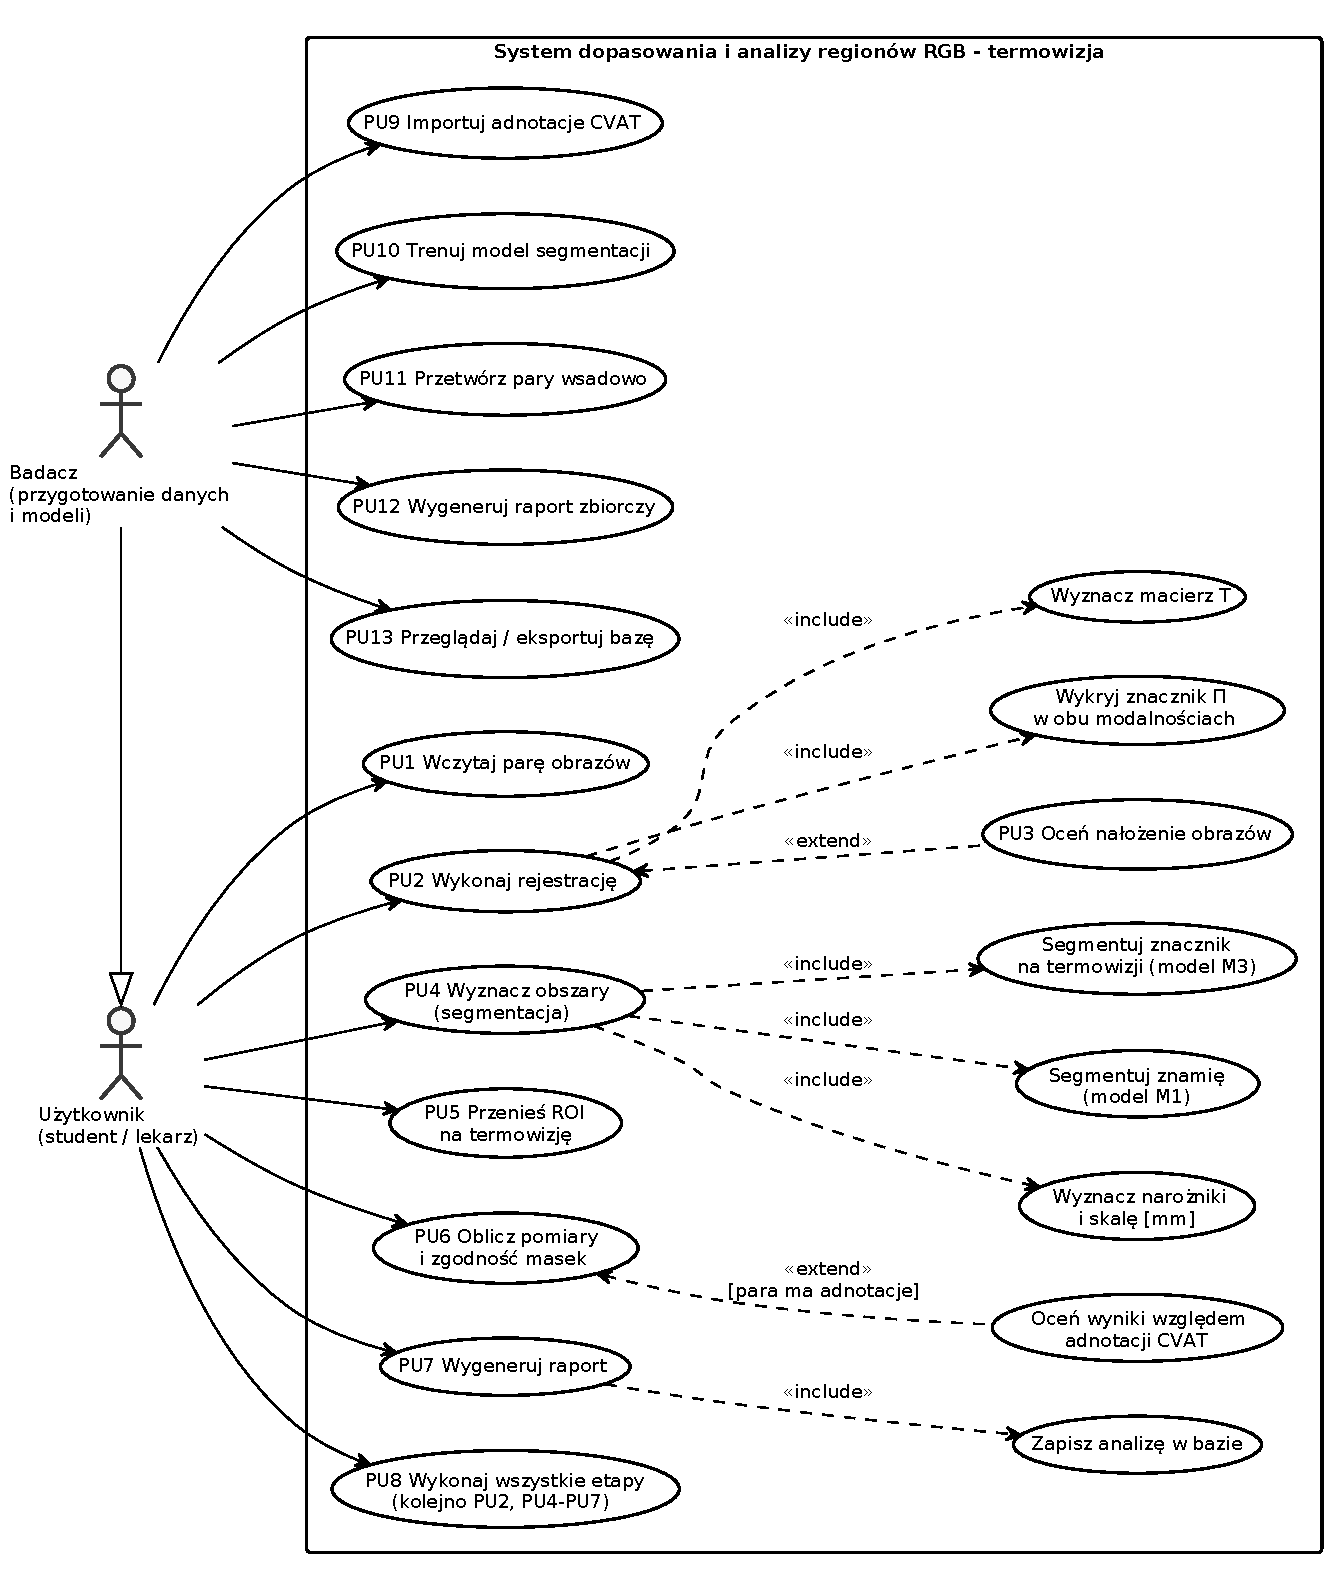
\includegraphics[width=0.85\textwidth]{rysunki/przypadki_uzycia.pdf}
  \caption{Diagram przypadków użycia systemu}
  \label{fig:przypadki-uzycia}
\end{figure}

Przypadek PU2 obejmuje (relacja \guillemotleft include\guillemotright) wykrycie znacznika w obu modalnościach i wyznaczenie macierzy $T$, a ocena nałożenia obrazów (PU3) stanowi jego opcjonalne rozszerzenie (relacja \guillemotleft extend\guillemotright). Ocena wyników względem adnotacji rozszerza przypadek PU6 wyłącznie wtedy, gdy para obrazów ma adnotacje. Scenariusz przypadku PU2 przedstawiono w tabeli~\ref{tab:scenariusz}.

\begin{table}[htbp]
  \centering
  \caption{Scenariusz przypadku użycia PU2 „Wykonaj rejestrację”}
  \label{tab:scenariusz}
  \small
  \begin{tabularx}{\textwidth}{>{\raggedright\arraybackslash}p{3.2cm} X}
    \toprule
    Aktor & Użytkownik \\
    Warunki początkowe & wczytano parę obrazów (PU1) \\
    Scenariusz główny & 1.~Użytkownik wybiera polecenie rejestracji. 2.~System wykrywa znacznik na obrazie termowizyjnym i na zdjęciu. 3.~System wyznacza wstępne dopasowanie kształtów znacznika. 4.~System doprecyzowuje transformację i wybiera jej model. 5.~System wyświetla nałożenie obrazów i zapisuje macierz $T$. \\
    Scenariusze alternatywne & 2a.~Znacznik nie zostaje wykryty -- system wyświetla komunikat i kończy przypadek. 2b.~Kształt wykrytego obiektu słabo odpowiada wzorcowi -- system wyświetla ostrzeżenie. 4a.~Homografia jest niestabilna -- system wybiera przekształcenie afiniczne. \\
    Warunki końcowe & macierz $T$ jest dostępna dla kolejnych etapów \\
    \bottomrule
  \end{tabularx}
\end{table}

\section{Architektura systemu}
\label{sec:architektura}

System zaprojektowano w architekturze potokowej, w której każdy etap korzysta z wyników poprzedniego (rys.~\ref{fig:potok}). Po wczytaniu pary obrazów system wyznacza macierz rejestracji, następnie -- niezależnie od siebie -- narożniki znacznika i skalę, maskę znamienia na zdjęciu oraz maskę znacznika na obrazie termowizyjnym. Kolejne etapy to przeniesienie obszarów przez macierz $T$, pomiary i ocena zgodności oraz raport.

\begin{figure}[htbp]
  \centering
  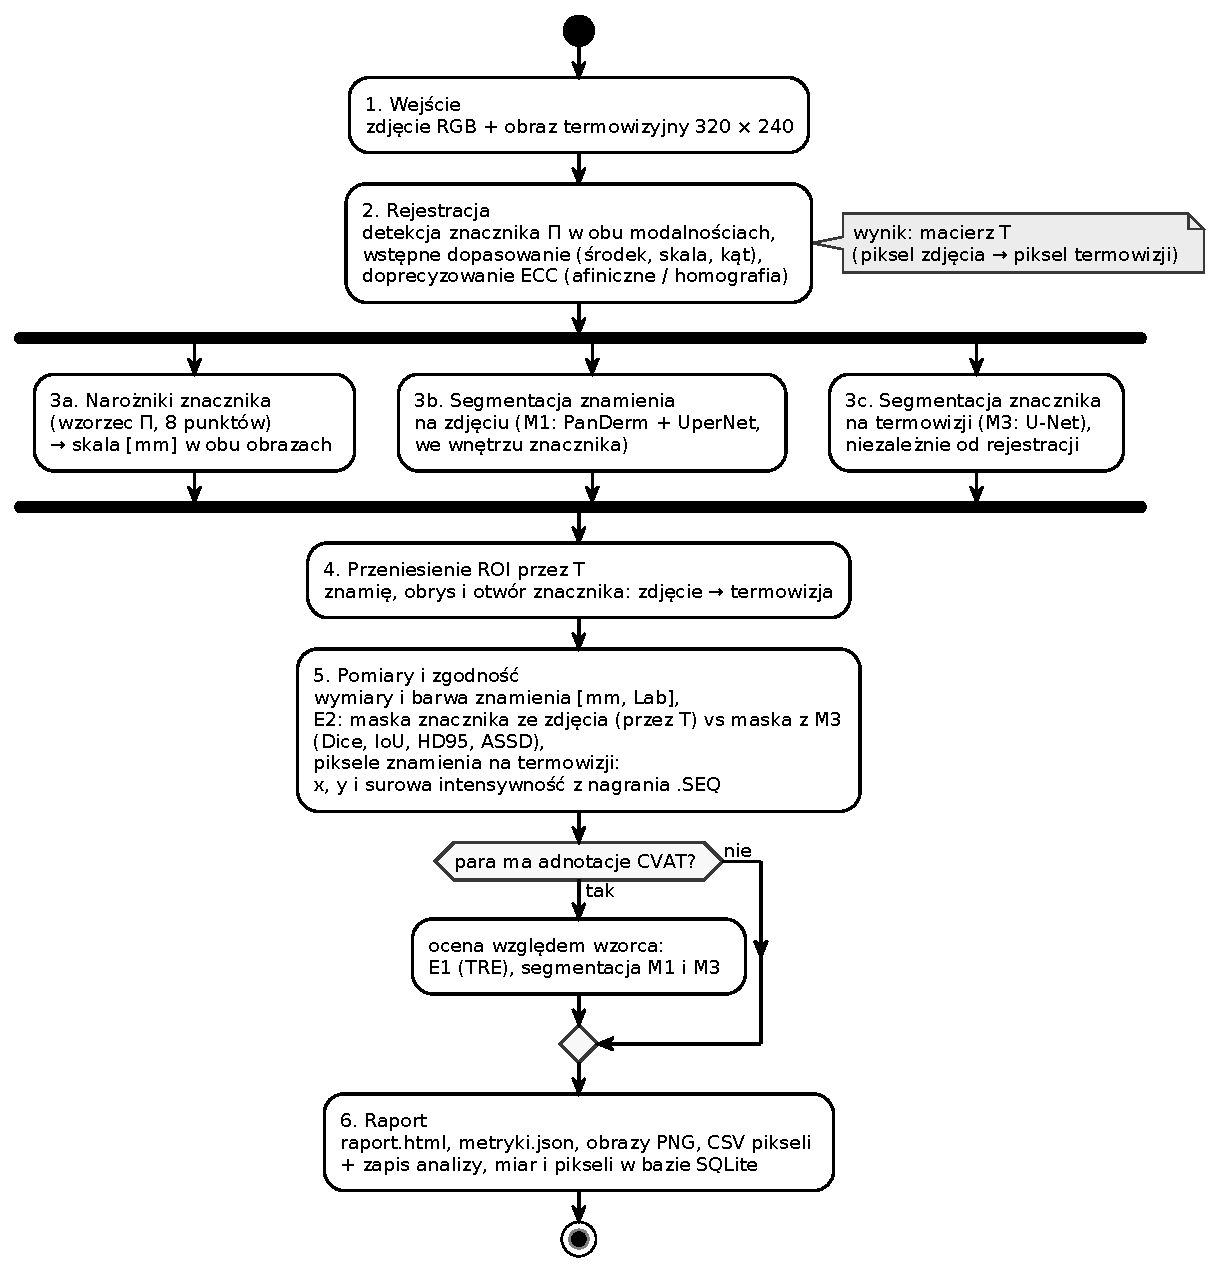
\includegraphics[width=0.6\textwidth]{rysunki/potok_przetwarzania.pdf}
  \caption{Potok przetwarzania pary obrazów (diagram aktywności UML)}
  \label{fig:potok}
\end{figure}

Podział systemu na warstwy przedstawiono na rysunku~\ref{fig:architektura}. Warstwę prezentacji tworzą aplikacja okienkowa i skrypty przetwarzania wsadowego. Obie korzystają z warstwy logiki, w której etapy potoku realizuje jedna klasa, dzięki czemu ten sam kod jest wykorzystywany zarówno w trybie interaktywnym, jak i wsadowym (WN8). Moduły obliczeniowe odpowiadają za rejestrację, segmentację znacznika na obrazie termowizyjnym, przeniesienie obszarów i pomiary oraz raport. Model segmentacji znamienia działa w osobnym środowisku z biblioteką PyTorch i jest uruchamiany jako odrębny proces, co pozwala zachować lekkie środowisko aplikacji (WN7). Warstwę danych tworzą pliki obrazów, masek i wyników, wagi modeli oraz baza danych przechowująca wyniki analiz.

\begin{figure}[htbp]
  \centering
  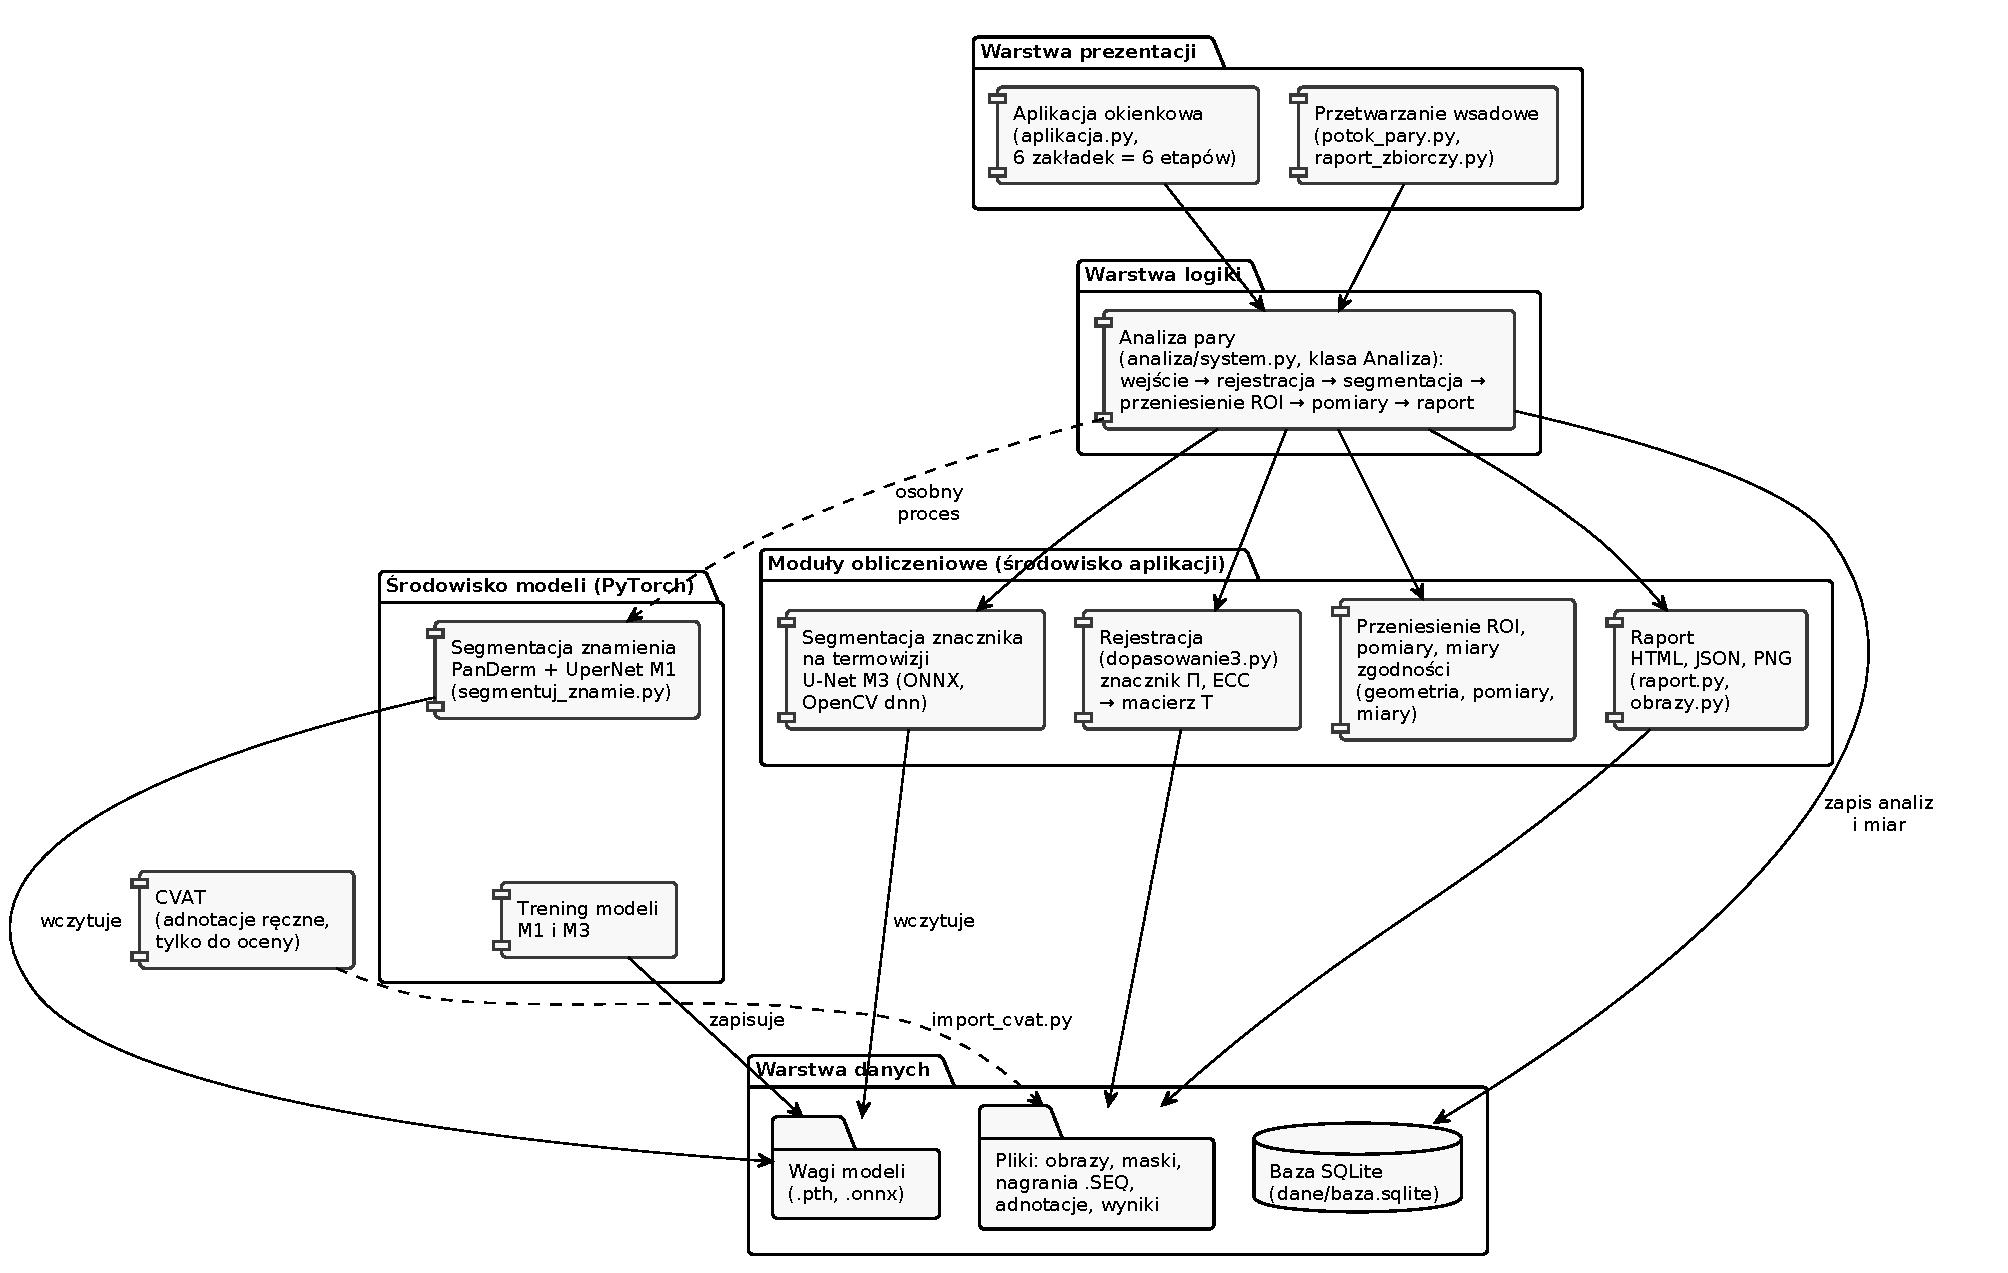
\includegraphics[width=\textwidth]{rysunki/architektura_systemu.pdf}
  \caption{Architektura systemu: warstwy, moduły obliczeniowe i środowiska uruchomieniowe}
  \label{fig:architektura}
\end{figure}

% =====================================================================
% Rozdział 4 – Projekt systemu (WZÓR, ok. 4,5 strony)
% Styl bezosobowy. Rysunki: rysunki/znacznik_pi_wymiary.pdf, rysunki/baza_erd.pdf (6 tabel, wersja 28.10),
% rysunki/diagram_klas.pdf (wersja 28.10); zrzut ekranu aplikacji – do wykonania (TODO poniżej).
% Plan i zwroty: materialy/06_plan_zwroty_rozdzialy_4_7.md.
% Wymaga pakietów: booktabs, tabularx.
% =====================================================================

\chapter{Projekt systemu}
\label{chap:projekt}

W rozdziale opisano decyzje projektowe, które pozwalają spełnić wymagania przedstawione w rozdziale~\ref{chap:analiza}: dobór technologii, projekt znacznika referencyjnego, bazy danych, struktury klas oraz interfejsu użytkownika.

\section{Dobór technologii}
\label{sec:technologie}

Przy wyborze technologii kierowano się dostępnością gotowych implementacji metod opisanych w rozdziale~\ref{chap:stan-wiedzy}, możliwością pracy bez procesora graficznego oraz prostotą instalacji na komputerze użytkownika. Wykorzystane technologie zestawiono w tabeli~\ref{tab:technologie}.

\begin{table}[htbp]
  \centering
  \caption{Technologie wykorzystane w systemie}
  \label{tab:technologie}
  \small
  \begin{tabularx}{\textwidth}{>{\raggedright\arraybackslash}p{3.0cm} >{\raggedright\arraybackslash}p{3.3cm} X}
    \toprule
    Element & Technologia & Uzasadnienie \\
    \midrule
    język programowania & Python 3.14 (aplikacja) & bogaty ekosystem bibliotek przetwarzania obrazów i uczenia maszynowego; jeden język dla aplikacji i modeli \\
    przetwarzanie obrazów i rejestracja & OpenCV 4.13, NumPy 2.4 & gotowa implementacja kryterium ECC~\cite{evangelidis2008}, operacji morfologicznych i wnioskowania sieci w formacie ONNX \\
    uczenie głębokie & PyTorch 2.11 (osobne środowisko, Python 3.12) & trening sieci U-Net i douczanie modelu PanDerm, którego wagi udostępniono dla tej biblioteki \\
    wnioskowanie sieci U-Net & ONNX + moduł \texttt{dnn} biblioteki OpenCV & uruchamianie modelu bez biblioteki PyTorch (WN7) \\
    interfejs graficzny & customtkinter 5.2 (nakładka na tkinter) & lekka biblioteka o otwartej licencji; tkinter jest częścią instalacji Pythona \\
    baza danych & SQLite & baza w jednym pliku, niewymagająca serwera, wystarczająca dla jednego użytkownika \\
    odczyt nagrań termowizyjnych & flirpy 0.3 & klatki i surowe wartości detektora z nagrań .SEQ kamery FLIR A320 (WF15) \\
    adnotacje & CVAT & oznaczanie masek i punktów (narożników) w przeglądarce \\
    raport & HTML, JSON, PNG & raport czytelny bez dodatkowego oprogramowania; wyniki w formacie do dalszej analizy \\
    metoda porównawcza & SimpleITK 2.5 & rejestracja z informacją wzajemną~\cite{zitova2003} w badaniu porównawczym \\
    \bottomrule
  \end{tabularx}
\end{table}

Rozważano także rejestrację bezpośrednio na intensywnościach obu obrazów z użyciem informacji wzajemnej~\cite{zitova2003,correlation-ratio} (metryka \texttt{MattesMutualInformation} biblioteki SimpleITK). Podejście to zastosowano we wcześniejszej wersji systemu i zachowano jako metodę porównawczą, natomiast w systemie docelowym transformację wyznacza się na maskach znacznika, zgodnie z wnioskami z przeglądu literatury (podrozdział~\ref{sec:modele-transformacji}). Zrezygnowano również z przechowywania wyników w plikach CSV na rzecz bazy danych, która zachowuje historię analiz i relacje między danymi.

\section{Projekt znacznika referencyjnego}
\label{sec:znacznik}

Znacznik referencyjny powinien spełniać następujące wymagania: być widoczny zarówno na zdjęciu, jak i na obrazie termowizyjnym; mieć kształt pozwalający jednoznacznie wyznaczyć położenie, skalę i kąt obrotu; zawierać punkty charakterystyczne umożliwiające wyznaczenie skali w milimetrach i ocenę błędu rejestracji; pozostawiać miejsce na znamię oraz być tani i łatwy do naklejenia.

Znacznik wykonano z taśmy pokrytej folią aluminiową. Na zdjęciu folia jest szara, o metalicznym połysku i teksturze załamań, a na obrazie termowizyjnym wyraźnie różni się od skóry, której emisyjność jest bliska jedności~\cite{infared-thermal-imaging}. Element aluminiowy (schłodzoną płytę) jako źródło kontrastu w obrazie termowizyjnym wykorzystano także w~\cite{gonzalezperez2021}.

Znacznik ma kształt litery $\Pi$ o wymiarach 35~$\times$~26~mm i szerokości paska 9~mm (rys.~\ref{fig:znacznik}). Otwór między ramionami ma wymiary 17~$\times$~17~mm (pole 289~mm$^2$) i wyznacza obszar zainteresowania, w którym umieszcza się znamię. Osiem narożników znacznika (P1--P8) służy do wyznaczenia homografii przekształcającej piksele na milimetry oraz do oceny błędu rejestracji. Kształt nie ma symetrii obrotowej, dzięki czemu kąt obrotu jest wyznaczany jednoznacznie w pełnym zakresie 360°. Znacznik jest jednak symetryczny względem osi pionowej, więc odbicie lustrzane obrazu dałoby fałszywe dopasowanie z zamienionymi ramionami; ponieważ żadna z kamer nie odwraca obrazu, przypadku tego nie rozpatruje się.

\begin{figure}[htbp]
  \centering
  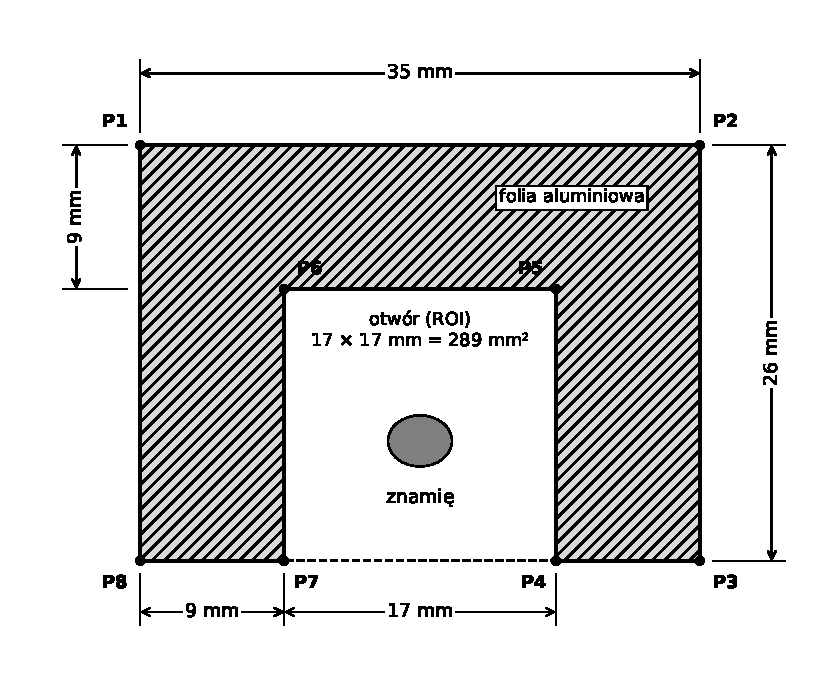
\includegraphics[width=0.6\textwidth]{rysunki/znacznik_pi_wymiary.pdf}
  \caption{Wymiary znacznika referencyjnego $\Pi$; P1--P8 -- narożniki wykorzystywane do wyznaczenia skali i błędu rejestracji}
  \label{fig:znacznik}
\end{figure}

We wcześniejszej wersji systemu stosowano znaczniki o dowolnym kształcie, bez wyróżnionych punktów, co uniemożliwiało wyznaczenie skali w milimetrach i niezależną ocenę dokładności rejestracji. Znany kształt znacznika $\Pi$ pozwala natomiast porównywać wykryte maski ze wzorcem i ostrzegać o niepewnej detekcji.

\section{Projekt bazy danych}
\label{sec:baza}

Baza danych przechowuje informacje o zbiorze (znamiona, pary obrazów, adnotacje) oraz wyniki wszystkich analiz. Pliki obrazów, masek i raportów pozostają w folderach, a baza zawiera ich ścieżki względne. Rozwiązanie to ogranicza rozmiar bazy i pozwala przeglądać pliki bez dodatkowych narzędzi. Model danych przedstawiono na diagramie związków encji (rys.~\ref{fig:erd}), a opis tabel -- w tabeli~\ref{tab:baza}.

\begin{figure}[htbp]
  \centering
  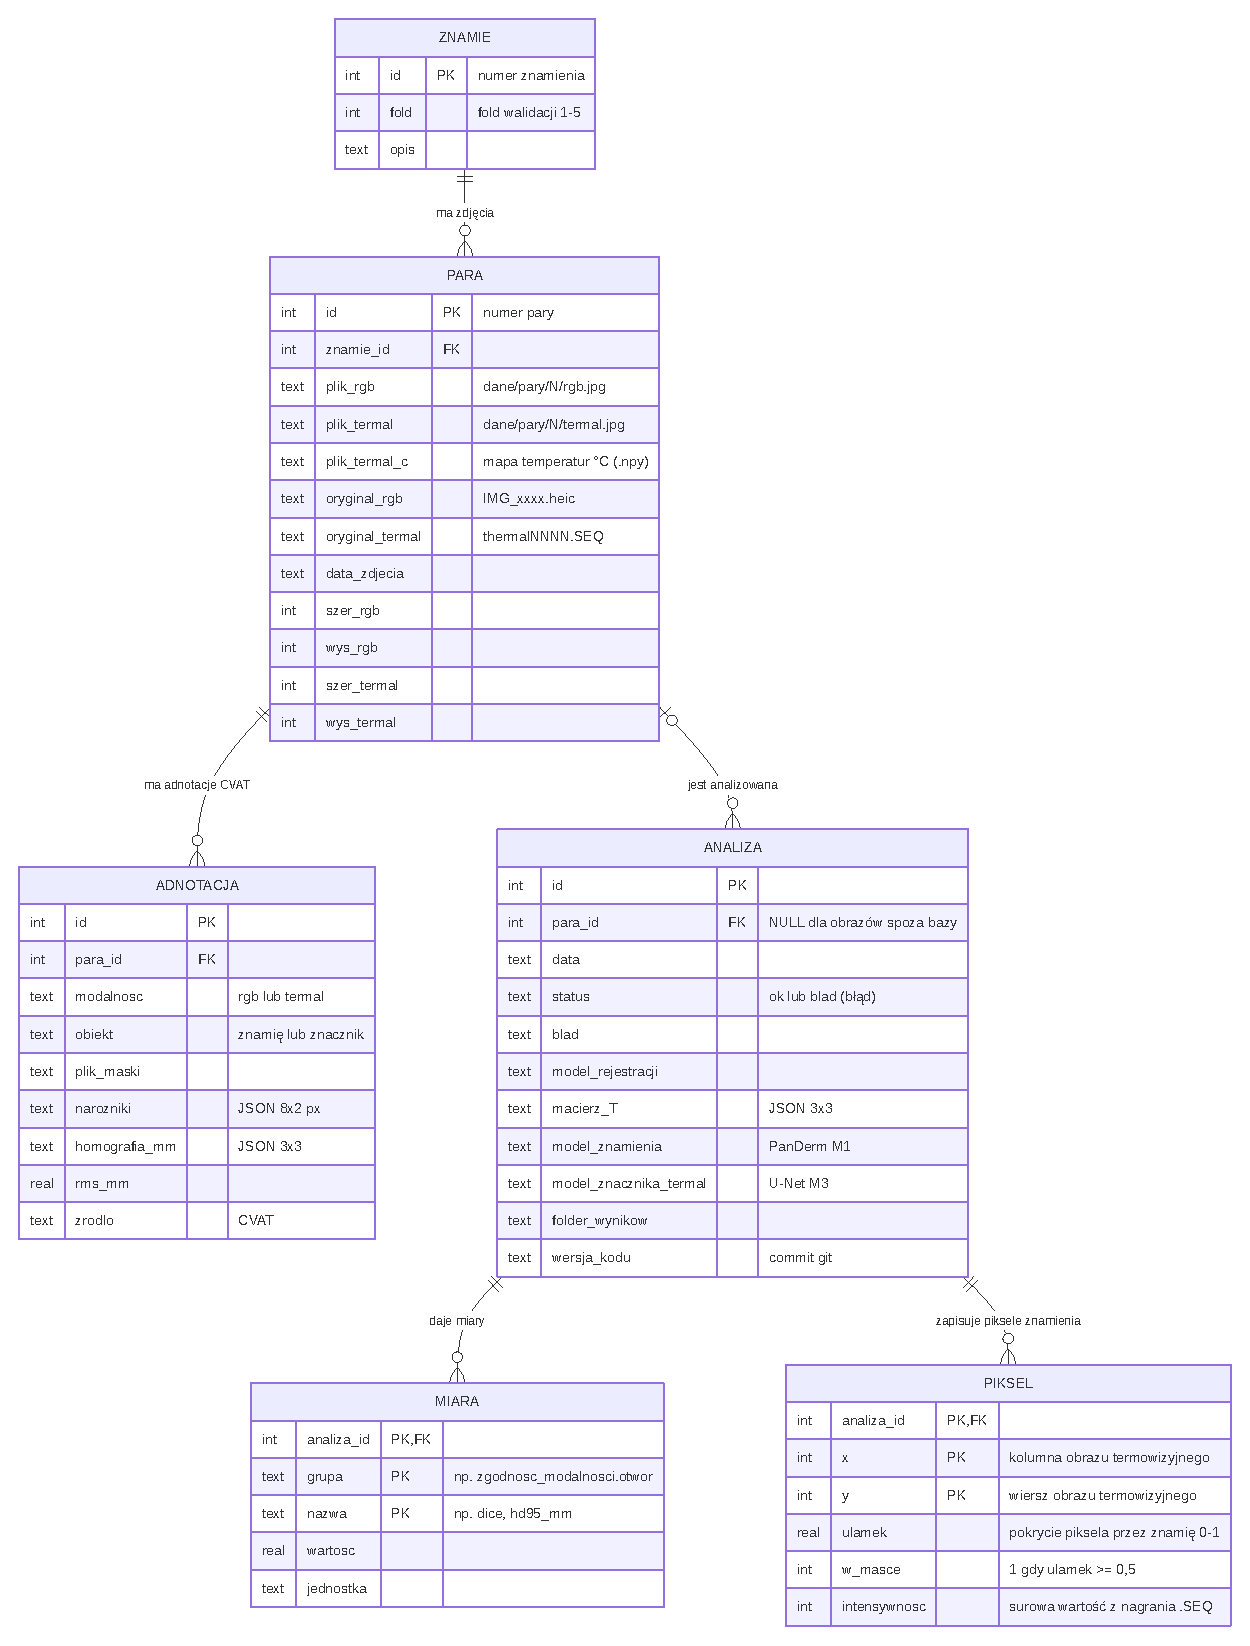
\includegraphics[width=0.62\textwidth]{rysunki/baza_erd.pdf}
  \caption{Diagram związków encji bazy danych systemu}
  \label{fig:erd}
\end{figure}

\begin{table}[htbp]
  \centering
  \caption{Tabele bazy danych}
  \label{tab:baza}
  \small
  \begin{tabularx}{\textwidth}{l X}
    \toprule
    Tabela & Zawartość \\
    \midrule
    \texttt{znamie} & numer znamienia i numer foldu walidacji krzyżowej \\
    \texttt{para} & ścieżki zdjęcia i obrazu termowizyjnego, nazwy plików oryginalnych, data wykonania zdjęcia, rozdzielczości; klucz obcy do tabeli \texttt{znamie} \\
    \texttt{adnotacja} & maski i narożniki znacznika z programu CVAT oraz homografia piksele--milimetry dla danej modalności \\
    \texttt{analiza} & każde uruchomienie analizy: data, status, użyte modele, macierz $T$, folder wyników i wersja kodu \\
    \texttt{miara} & wszystkie wyniki liczbowe analizy w postaci: grupa, nazwa, wartość, jednostka \\
    \texttt{piksel} & piksele obrazu termowizyjnego objęte znamieniem przeniesionym ze zdjęcia: współrzędne $x$, $y$, ułamek pokrycia, przynależność do maski i surowa intensywność z nagrania \\
    \bottomrule
  \end{tabularx}
\end{table}

Tabele połączono relacjami jeden do wielu: znamię ma wiele par obrazów, para -- wiele adnotacji i analiz, a analiza -- wiele miar i wiele pikseli znamienia. Tabelę \texttt{miara} zaprojektowano w układzie „długim” (jedna wartość w wierszu), dzięki czemu dodanie nowej miary nie wymaga zmiany schematu bazy. Dodatkowo zdefiniowano dwa widoki: \texttt{ostatnia\_analiza}, wskazujący najnowszą udaną analizę każdej pary, oraz \texttt{wyniki\_par}, łączący jej miary z numerem znamienia i foldu. Tabela \texttt{piksel} ma klucz główny złożony z identyfikatora analizy i współrzędnych piksela, co wyklucza powtórzenie piksela w jednej analizie i pozwala pobrać piksele znamienia jednym zapytaniem (WF15). Schemat bazy ma numer wersji; przy otwarciu bazy w starszej wersji brakujące tabele są tworzone automatycznie, bez utraty zapisanych analiz. Zapis do bazy następuje automatycznie po wygenerowaniu raportu (WF12, WN9).

\section{Diagram klas}
\label{sec:klasy}

Strukturę statyczną systemu przedstawiono na diagramie klas (rys.~\ref{fig:klasy}). Dla czytelności pominięto metody pomocnicze. Centralną klasą systemu jest \texttt{Analiza}, która przechowuje stan analizy jednej pary obrazów -- obrazy, macierz $T$, maski, narożniki, surowe wartości detektora, piksele znamienia i wyniki -- a jej metody odpowiadają kolejnym etapom potoku przetwarzania. Klasa \texttt{Aplikacja} realizuje interfejs graficzny i korzysta z obiektu klasy \texttt{Analiza}; podglądy obrazów realizuje klasa \texttt{Podglad}. Zapis wyników zapewnia klasa \texttt{Baza}, a niepowodzenia etapów są zgłaszane wyjątkiem \texttt{BladEtapu}, którego treść jest wyświetlana użytkownikowi (WN6).

\begin{figure}[htbp]
  \centering
  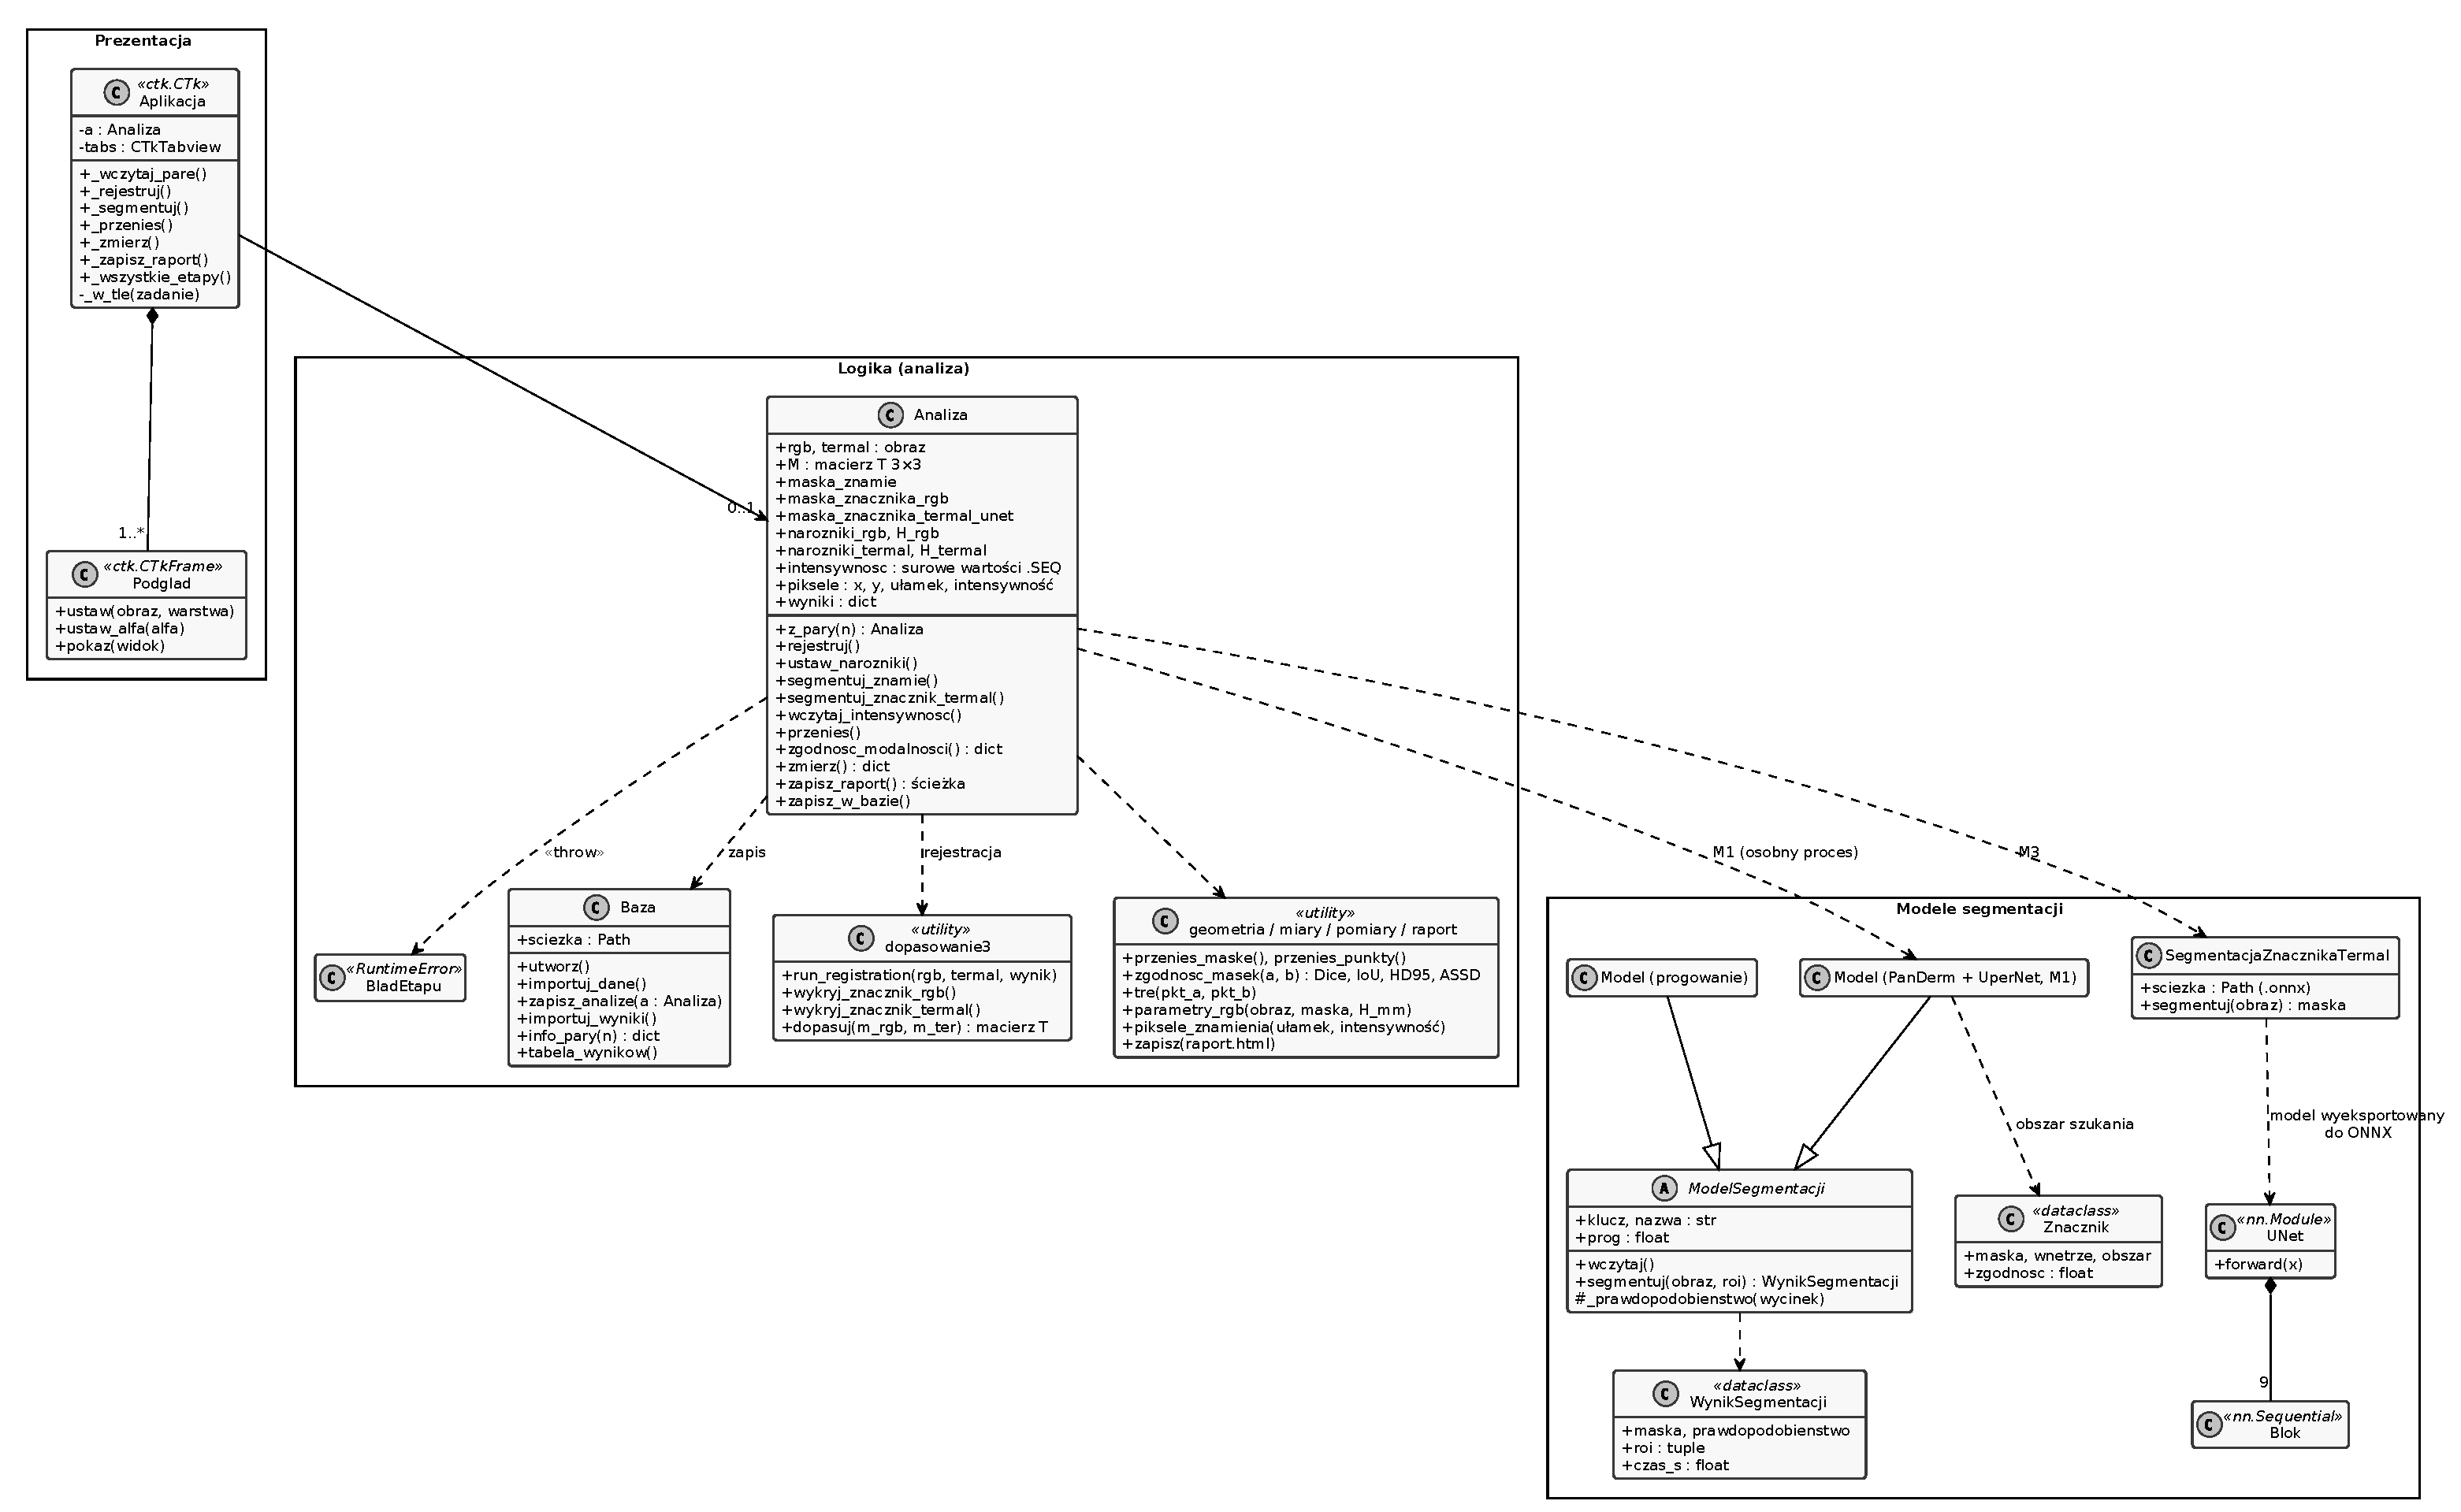
\includegraphics[width=\textwidth]{rysunki/diagram_klas.pdf}
  \caption{Diagram klas systemu (z pominięciem metod pomocniczych)}
  \label{fig:klasy}
\end{figure}

Modele segmentacji zdjęć dziedziczą po klasie abstrakcyjnej \texttt{ModelSegmentacji}, która definiuje wspólny interfejs wczytania modelu i segmentacji. Pozwala to dodawać kolejne modele bez zmiany pozostałych części systemu. Segmentację znacznika na obrazie termowizyjnym realizuje klasa \texttt{SegmentacjaZnacznikaTermal}, wykorzystująca sieć \texttt{UNet} wyeksportowaną do formatu ONNX. Moduły realizujące rejestrację, przekształcenia geometryczne, miary i raport zaimplementowano jako zbiory funkcji, oznaczone na diagramie stereotypem \guillemotleft utility\guillemotright.

\section{Projekt interfejsu użytkownika}
\label{sec:interfejs}

Interfejs zaprojektowano tak, aby odzwierciedlał kolejność etapów przetwarzania. Okno aplikacji składa się z czterech obszarów (rys.~\ref{fig:interfejs}): paska sześciu etapów (Dane, Rejestracja, Segmentacja, Przeniesienie ROI, Pomiary, Raport), panelu sterowania po lewej stronie, podglądów obrazów po prawej oraz paska stanu z dziennikiem zdarzeń w dolnej części okna.

\begin{figure}[htbp]
  \centering
  % TODO: wstawić zrzut ekranu zakładki „2. Rejestracja” (para 14) z oznaczonymi obszarami 1–4:
  % \includegraphics[width=\textwidth]{rysunki/interfejs_rejestracja.png}
  \fbox{\parbox[c][5cm][c]{0.9\textwidth}{\centering Zrzut ekranu aplikacji -- do wstawienia}}
  \caption{Okno aplikacji -- zakładka rejestracji: 1~--~pasek etapów, 2~--~panel sterowania, 3~--~podgląd nałożenia obrazów, 4~--~pasek stanu i dziennik zdarzeń}
  \label{fig:interfejs}
\end{figure}

Każda zakładka kończy się przyciskiem przejścia do kolejnego etapu, a przyciski etapów, których nie można jeszcze wykonać, są nieaktywne, co zapobiega uruchomieniu etapu bez wyników poprzedniego. Podglądy obrazów umożliwiają powiększanie (kółko myszy), przesuwanie (przeciąganie) i powrót do widoku początkowego (dwukrotne kliknięcie), a nałożenie obrazów ma regulowaną przezroczystość (WF3). Obliczenia są wykonywane w osobnym wątku, dzięki czemu interfejs pozostaje responsywny, a postęp jest widoczny na pasku stanu i w dzienniku (WN3). W zakładce pomiarów wybranie nazwy wielkości wyświetla jej objaśnienie, a w zakładce raportu można przejrzeć obrazy raportu, w tym piksele znamienia na obrazie termowizyjnym. Dane można wczytać na dwa sposoby: wybierając numer pary ze zbioru albo dwa dowolne pliki (WF1); dostępne jest też polecenie wykonania wszystkich etapów (WF13). Szczegółowy opis obsługi zawiera instrukcja użytkownika (Dodatek~A).

% =====================================================================
% Rozdział 5 – Implementacja (WZÓR, ok. 6 stron)
% Styl bezosobowy. Klucze \cite{} – literatura_wzor.bib (klucze z bibliografii autora).
% Rysunki: rysunki/rejestracja_para14.pdf, rysunki/panderm_trening.png.
% Wymaga pakietów: booktabs, tabularx, amsmath, algorithm, algpseudocode (opcja noend) – polskie
% nazwy w preambule (wzor_podglad.tex). Plan i zwroty: materialy/06_plan_zwroty_rozdzialy_4_7.md.
% Przy braku miejsca: usuń rys. fig:panderm-trening (wynik testu ISIC zostaje w tekście).
% =====================================================================

\chapter{Implementacja}
\label{chap:implementacja}

W rozdziale opisano implementację modułów systemu: przygotowanie danych, rejestrację, modele segmentacji, przeniesienie obszarów wraz z zapisem pikseli znamienia, pomiary oraz bazę danych, raport i aplikację. System zaimplementowano w języku Python; instalację środowisk i strukturę kodu opisano w dokumentacji technicznej (Dodatek~B).

\section{Akwizycja i przygotowanie danych}
\label{sec:dane}

Zbiór danych zebrano w jednej serii pomiarowej 23 października 2026~r. Obejmuje on 94 pary obrazów przedstawiających 34 znamiona; każde znamię sfotografowano dwa lub trzy razy, zmieniając obrót znacznika, odległość i kąt wykonania zdjęcia. Zdjęcia wykonano telefonem w formacie HEIC i przekonwertowano do formatu JPG (dłuższy bok 1104--3274 pikseli). Obrazy termowizyjne zarejestrowano kamerą FLIR A320 z obiektywem 18~mm jako nagrania .SEQ o rozdzielczości 320~$\times$~240 pikseli. Z pierwszej klatki każdego nagrania wyznaczono:
\begin{itemize}
  \item obraz podglądowy z paletą barw, znormalizowany do zakresu między 2. a 98. percentylem wartości nagrania -- wykorzystywany w rejestracji i wizualizacji;
  \item macierz surowych wartości detektora (liczby całkowite 16-bitowe), wykorzystywaną jako intensywność pikseli znamienia (WF15);
  \item pomocniczo -- mapę temperatur obliczoną z parametrów zapisanych w nagraniu przy emisyjności skóry 0,98~\cite{infared-thermal-imaging}.
\end{itemize}
Przy odczycie usuwano dolne wiersze zawierające dane telemetryczne kamery. Zgodność pikseli wszystkich reprezentacji sprawdzono współczynnikiem korelacji rang, który dla każdej z 94 par wyniósł co najmniej 0,95.

Ręczne adnotacje wykonano w programie CVAT: maskę znamienia na zdjęciu, maski znacznika na obu obrazach oraz osiem narożników znacznika w każdej modalności. Z narożników wyznaczono homografię przekształcającą piksele na milimetry w płaszczyźnie znacznika. Adnotacje wykorzystano wyłącznie do oceny wyników oraz do uczenia modelu M3. Na potrzeby walidacji krzyżowej zbiór podzielono na pięć foldów według znamion, a nie zdjęć, aby zdjęcia tego samego znamienia nie trafiały jednocześnie do zbioru uczącego i testowego.

\section{Moduł rejestracji}
\label{sec:impl-rejestracja}

Rejestrację zrealizowano zgodnie z założeniem przyjętym w rozdziale~\ref{chap:projekt}: transformację wyznacza się na podstawie znacznika $\Pi$, a nie całej sceny. Przebieg metody przedstawiono w postaci pseudokodu (algorytm~\ref{alg:rejestracja}), a jej wynik dla przykładowej pary -- na rysunku~\ref{fig:rejestracja-para}.

\subsection{Detekcja znacznika}

Na obrazie termowizyjnym folia odbija promieniowanie otoczenia, dlatego jest ciemniejsza od skóry albo -- przy odbiciach obiektów o różnej temperaturze -- silnie teksturowana, podczas gdy skóra jest gładka. Kandydatów na znacznik wyznaczono jako spójne obszary ciemniejsze od skóry (progi 0,5, 0,65 i 0,8 wartości 70. percentyla jasności obrazu) lub o lokalnym odchyleniu standardowym jasności większym niż 6, 10 albo 15, po otwarciu i zamknięciu morfologicznym. Spośród kandydatów wybierano obszar najbardziej podobny do wzorca $\Pi$; miarą podobieństwa jest indeks Jaccarda (IoU) kandydata i wzorca o tym samym polu i środku masy, maksymalizowany względem kąta obrotu w zakresie 0--360° z krokiem 4°. Krawędź folii, rozmytą przez optykę kamery, wyznaczono z dokładnością subpikselową, przyjmując w pasie $\pm 4$~pikseli wokół krawędzi próg w połowie między jasnością folii i skóry.

Na zdjęciu folia jest chłodniejsza w barwie od skóry -- ma mniejszą sumę składowych $a^*$ i $b^*$ przestrzeni L*a*b* niż mediana skóry -- i ma teksturę załamań. Kandydatów wyznaczono przy kilku progach z mapy barwy, mapy tekstury (odchylenie standardowe w oknie 7~$\times$~7 pikseli) oraz ich połączenia, a wybór przebiega tak samo jak na obrazie termowizyjnym. Krawędź folii doprecyzowano segmentacją interaktywną z biblioteki OpenCV, akceptowaną tylko wtedy, gdy nie pogarsza zgodności kształtu z wzorcem. Detekcję na zdjęciu wykonuje się w skali roboczej, w której dłuższy bok ma 1000 pikseli. Jeżeli zgodność wykrytego obiektu z wzorcem jest mniejsza niż 0,65, system zgłasza ostrzeżenie (WN6).

\subsection{Dopasowanie wstępne i doprecyzowanie metodą ECC}

Dopasowanie wstępne jest przekształceniem przez podobieństwo: przesunięcie wynika ze środków mas masek znacznika, skala -- z pierwiastka stosunku ich pól, a kąt -- z maksimum IoU masek po obrocie (krok 2°, a następnie $\pm 2^\circ$ z krokiem 0,25°). Transformację doprecyzowano, maksymalizując kryterium ECC~\cite{evangelidis2008} funkcją \texttt{findTransformECC} biblioteki OpenCV. Kryterium obliczano nie na intensywnościach obrazów, lecz na maskach znacznika rozmytych filtrem Gaussa, co sprowadza problem wielomodalny do jednomodalnego (podrozdział~\ref{sec:modele-transformacji}). Optymalizację prowadzono od dużego do małego rozmycia: dla przekształcenia afinicznego przy $\sigma = 6$, 3 i 1,5~piksela, a następnie dla homografii przy $\sigma = 3$ i 1,5~piksela (do 200 iteracji, $\varepsilon = 10^{-6}$), na wycinku obejmującym znacznik z marginesem 30\%. Rozmycie poszerza obszar zbieżności metody gradientowej, a jego stopniowe zmniejszanie zwiększa dokładność.

\subsection{Wybór modelu przekształcenia}

Domyślnie przyjmowano przekształcenie afiniczne. Homografię wybierano wtedy, gdy zmniejszała średni błąd krawędzi masek o ponad 5\% i była stabilna, tzn. lokalna skala pola w narożnikach kadru zdjęcia różniła się od skali w środku znacznika najwyżej dwukrotnie. Warunek ten odrzuca homografie dopasowane do znacznika, ale zniekształcające pozostałą część obrazu. W zbiorze 92 przeanalizowanych par homografię wybrano 65 razy, a przekształcenie afiniczne -- 27 razy. Wynikiem modułu jest macierz $T$ przekształcająca piksel zdjęcia na piksel obrazu termowizyjnego, obraz termowizyjny w geometrii zdjęcia (z kanałem przezroczystości wyznaczającym pole widzenia kamery) oraz nałożenie obu obrazów.

\begin{algorithm}[htbp]
  \caption{Rejestracja zdjęcia i obrazu termowizyjnego na podstawie znacznika $\Pi$}
  \label{alg:rejestracja}
  \small
  \begin{algorithmic}[1]
    \Require zdjęcie $I_R$, obraz termowizyjny $I_T$, wzorzec $\Pi$
    \Ensure macierz $T$ (piksel $I_R$ $\to$ piksel $I_T$), model przekształcenia
    \State $M_T \gets$ \Call{WykryjZnacznik}{$I_T$} \Comment{obszary ciemne lub teksturowane}
    \State $M_R \gets$ \Call{WykryjZnacznik}{$I_R$} \Comment{obszary chłodne w barwie lub teksturowane}
    \If{$\mathrm{IoU}(M_R, \Pi) < 0{,}65$ \textbf{lub} $\mathrm{IoU}(M_T, \Pi) < 0{,}65$}
      \State zgłoś ostrzeżenie o niepewnej detekcji znacznika
    \EndIf
    \State $W_0 \gets$ podobieństwo: środki mas, skala $\sqrt{|M_T| / |M_R|}$, kąt $\arg\max_\alpha \mathrm{IoU}\big(\mathrm{obrót}_\alpha(M_R), M_T\big)$
    \State $W_A \gets W_0$
    \For{$\sigma \in (6;\ 3;\ 1{,}5)$}
      \State $W_A \gets \mathrm{ECC}_{\mathrm{afiniczne}}(G_\sigma * M_R,\ G_\sigma * M_T,\ W_A)$
    \EndFor
    \State $W_H \gets W_A$
    \For{$\sigma \in (3;\ 1{,}5)$}
      \State $W_H \gets \mathrm{ECC}_{\mathrm{homografia}}(G_\sigma * M_R,\ G_\sigma * M_T,\ W_H)$
    \EndFor
    \If{$e(W_H) < 0{,}95\, e(W_A)$ \textbf{oraz} $W_H$ stabilna} \Comment{$e$ -- średni błąd krawędzi masek}
      \State \Return $W_H$, homografia
    \Else
      \State \Return $W_A$, przekształcenie afiniczne
    \EndIf
  \end{algorithmic}
\end{algorithm}

\begin{figure}[htbp]
  \centering
  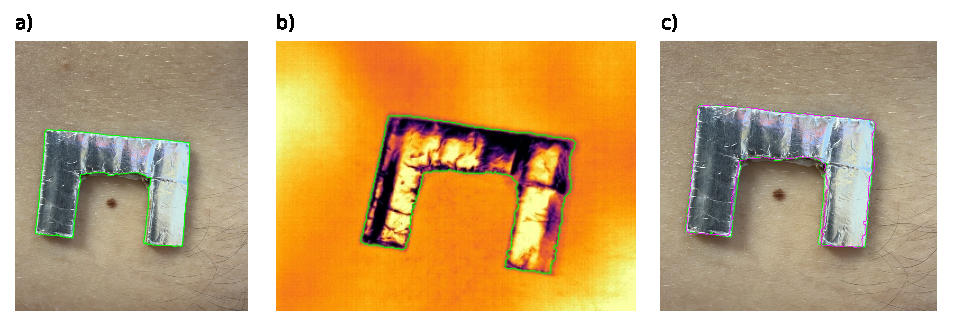
\includegraphics[width=0.92\textwidth]{rysunki/rejestracja_para14.pdf}
  \caption{Rejestracja pary 14: a)~folia wykryta na zdjęciu, b)~folia wykryta na obrazie termowizyjnym, c)~kontur folii ze zdjęcia (zielony) i kontur folii z obrazu termowizyjnego przeniesiony przekształceniem odwrotnym do $T$ (fioletowy). Źródło: opracowanie własne}
  \label{fig:rejestracja-para}
\end{figure}

\section{Modele segmentacji}
\label{sec:impl-segmentacja}

Zgodnie z celem pracy każda modalność ma własny model segmentacji. Na zdjęciu segmentowane jest znamię (model M1), a na obrazie termowizyjnym -- znacznik (model M3), ponieważ znamię nie jest na nim widoczne. Parametry uczenia obu modeli zestawiono w tabeli~\ref{tab:uczenie}.

\begin{table}[htbp]
  \centering
  \caption{Parametry uczenia modeli segmentacji}
  \label{tab:uczenie}
  \small
  \begin{tabularx}{\textwidth}{>{\raggedright\arraybackslash}p{2.6cm} >{\raggedright\arraybackslash}X >{\raggedright\arraybackslash}X}
    \toprule
    Parametr & M1: PanDerm + UperNet & M3: U-Net \\
    \midrule
    zadanie & znamię na zdjęciu & znacznik na obrazie termowizyjnym \\
    dane uczące & ISIC 2018 Task 1: 2594 / 100 / 1000 obrazów & 94 obrazy własne, 5 foldów według znamion \\
    wejście & 224~$\times$~224, RGB & 240~$\times$~320, skala szarości \\
    architektura & koder ViT-L z wagami PanDerm, dekoder UperNet & U-Net, kanały 16--256, 1,94~mln parametrów \\
    funkcja straty & entropia krzyżowa & BCE + (1 $-$ miękki Dice) \\
    optymalizator & AdamW (8-bitowy), $\eta = 10^{-4}$, $\lambda = 0{,}05$ & AdamW, $\eta = 2\cdot10^{-3}$, $\lambda = 10^{-4}$ \\
    harmonogram & kosinusowy, 100 epok, wybór epoki na zbiorze walidacyjnym & kosinusowy, 60 epok, bez wyboru epoki \\
    paczka & 2 & 8 \\
    augmentacja & zmiany barw, skala szarości, autokontrast, negatyw & obrót 0--360°, skala 0,75--1,3, przesunięcie, odbicia, korekcja gamma, kontrast, rozmycie, szum \\
    uruchamianie & PyTorch, osobny proces & ONNX + OpenCV w aplikacji \\
    \bottomrule
  \end{tabularx}
\end{table}

\subsection{Model M1 -- znamię na zdjęciu}

Model M1 składa się z kodera PanDerm (transformer wizyjny ViT-L) z wagami udostępnionymi przez autorów~\cite{yan2025panderm} oraz dekodera UperNet~\cite{xiao2018upernet}. Model douczono na zbiorze ISIC 2018 Task~1~\cite{codella2019} według procedury autorów modelu PanDerm; ze względu na kartę graficzną o pamięci 8~GB zastosowano 8-bitową wersję optymalizatora AdamW i obliczenia w formacie bfloat16. Model wybrano po 11. epoce, w której indeks Jaccarda na zbiorze walidacyjnym był największy (rys.~\ref{fig:panderm-trening}). Na zbiorze testowym (1000 obrazów) uzyskano współczynnik Dice'a 0,899 i indeks Jaccarda 0,833.

% OPCJA (ok. 0,4 s.): przy braku miejsca usuń rysunek i odwołanie do niego -- wynik testu ISIC zostaje w tekście.
\begin{figure}[htbp]
  \centering
  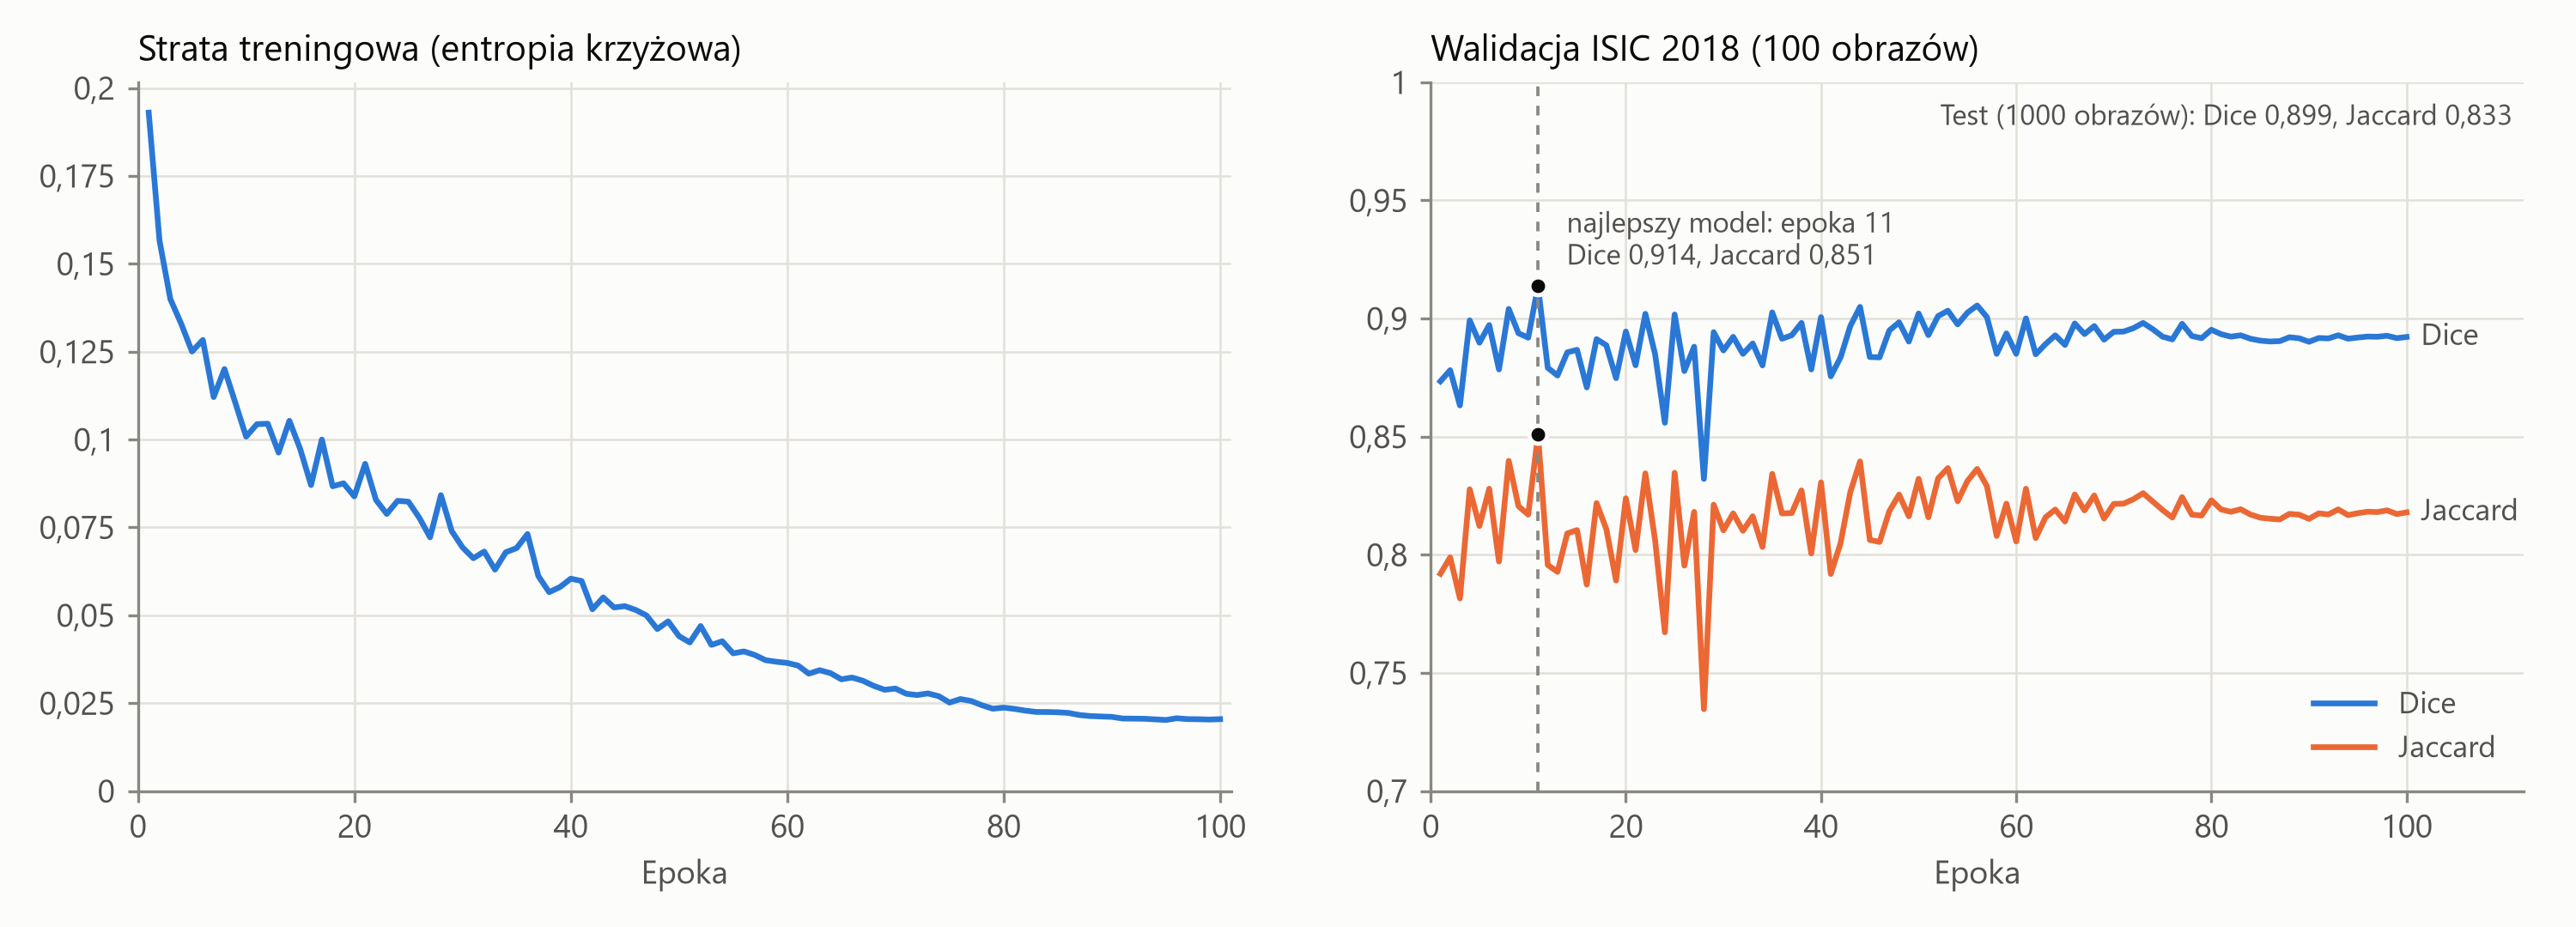
\includegraphics[width=0.85\textwidth]{rysunki/panderm_trening.png}
  \caption{Douczanie modelu M1 na zbiorze ISIC 2018: strata na zbiorze uczącym (po lewej) oraz współczynnik Dice'a i indeks Jaccarda na zbiorze walidacyjnym (po prawej). Źródło: opracowanie własne}
  \label{fig:panderm-trening}
\end{figure}

Bezpośrednie zastosowanie modelu do zdjęć z telefonu dawało maski znacznie zawyżone. Przyczyną jest przesunięcie dziedziny: w obrazach dermatoskopowych ISIC znamię zajmuje około połowy kadru, a na zdjęciu ze znacznikiem znamię o średnicy 1--4~mm zajmuje niewielką część otworu o boku 17~mm. Dlatego obszar segmentacji ograniczono do otworu znacznika poszerzonego o 8\% (piksele folii zastępuje się medianą barwy skóry), a segmentację podzielono na dwa kroki. Najpierw wyznacza się do trzech kandydatów na znamię jako plamy ciemniejsze od lokalnego tła skóry: jasność po domknięciu morfologicznym o promieniu ok. 0,2~mm, usuwającym włosy, porównuje się z medianą w oknie 8~mm, odrzucając pasy wzdłuż folii i kształty wydłużone. Następnie model segmentuje kadr wokół każdego kandydata, dobrany tak jak w danych uczących ISIC (znamię zajmuje ok. 53\% dłuższego boku kadru), a spośród wyników wybiera się maskę o największym kontraście brzegu, czyli różnicy jasności wewnątrz maski i w pasie 0,4~mm na zewnątrz niej. Model M1 działa w osobnym środowisku z biblioteką PyTorch i jest uruchamiany przez aplikację jako odrębny proces (WN7).

\subsection{Model M3 -- znacznik na obrazie termowizyjnym}

Model M3 jest siecią U-Net~\cite{ronneberger2015} zmniejszoną do rozmiaru zbioru: koder i dekoder mają cztery poziomy o liczbie kanałów 16, 32, 64 i 128, a najgłębsza warstwa -- 256 kanałów. Każdy z dziewięciu bloków składa się z dwóch splotów 3~$\times$~3 z normalizacją wsadową i funkcją aktywacji ReLU; sieć ma 1,94~mln parametrów. Wejściem jest obraz termowizyjny w skali szarości, standaryzowany osobno dla każdego obrazu, a wyjściem -- mapa prawdopodobieństwa przynależności piksela do folii, progowana wartością 0,5. Sieć uczono na 94 maskach znacznika z programu CVAT w 5-krotnej walidacji krzyżowej według znamion; dla każdej pary system używa modelu foldu, w którym była ona w zbiorze testowym, a dla obrazów spoza zbioru -- modelu uczonego na wszystkich parach. Liczbę epok ustalono z góry, bez wyboru epoki na zbiorze testowym, aby nie zawyżać wyników, a niewielki rozmiar zbioru kompensowano silną augmentacją. Wytrenowane sieci wyeksportowano do formatu ONNX i uruchamia się je modułem \texttt{dnn} biblioteki OpenCV, bez biblioteki PyTorch; segmentacja jednego obrazu trwa ok.~67~ms na procesorze (WN2). Model M3 nie uczestniczy w rejestracji, dlatego jego maska stanowi niezależny punkt odniesienia w badaniu E2.

\section{Przeniesienie obszarów i skala metryczna}
\label{sec:impl-przeniesienie}

Skalę metryczną wyznaczono z narożników znacznika. Wzorzec $\Pi$ o znanych wymiarach dopasowano do maski znacznika w każdej modalności (podobieństwo, a następnie ECC dla przekształcenia afinicznego i homografii), a osiem wierzchołków dopasowanego wzorca przyjęto za narożniki. Z narożników wyznaczono homografię $H$ przekształcającą piksele obrazu na milimetry w płaszczyźnie znacznika. Lokalny rozmiar piksela w danym punkcie jest pierwiastkiem z wartości bezwzględnej wyznacznika jakobianu $H$; dla obrazu termowizyjnego wynosi on 0,21--0,44~mm (mediana 0,28~mm).

Obszary przenoszono wektorowo (algorytm~\ref{alg:przeniesienie}). Kontur maski znamienia na zdjęciu, poszerzony o pół piksela (kontur prowadzony przez środki pikseli brzegowych zaniżałby pole), przekształcano macierzą $T$, a powstały wielokąt wypełniano w siatce czterokrotnie gęstszej niż piksele obrazu termowizyjnego. Średnia w bloku 4~$\times$~4 daje ułamek pokrycia każdego piksela przez znamię (wielokrotność 1/16). Pozwala to zachować kształt małego obszaru -- znamię obejmuje na obrazie termowizyjnym od 10 do 290 pikseli -- przy błędzie pola rzędu 1\%. W ten sam sposób przenoszono obrys i otwór znacznika.

Dla każdego piksela obrazu termowizyjnego o niezerowym ułamku pokrycia system zapisuje jego współrzędne $x$ (kolumna) i $y$ (wiersz), ułamek pokrycia oraz surową intensywność odczytaną z nagrania .SEQ (WF15). Piksel uznaje się za należący do znamienia, gdy znamię pokrywa co najmniej połowę jego pola, co odpowiada przeniesieniu maski binarnej. Pozostałe piksele są zapisywane wraz z ułamkiem pokrycia, co umożliwia analizę z wagami. Lista pikseli trafia do pliku CSV i do tabeli \texttt{piksel} bazy danych.

\begin{algorithm}[htbp]
  \caption{Przeniesienie znamienia na obraz termowizyjny i zapis pikseli}
  \label{alg:przeniesienie}
  \small
  \begin{algorithmic}[1]
    \Require maska znamienia $Z$ na zdjęciu, macierz $T$, surowe wartości detektora $I$ ($320 \times 240$)
    \Ensure lista pikseli $(x, y, u, m, I(x, y))$
    \State $K \gets$ kontur maski $Z$ poszerzony o pół piksela
    \State $K' \gets T \cdot K$ \Comment{wierzchołki we współrzędnych obrazu termowizyjnego}
    \State $G \gets$ wypełnienie wielokąta $K'$ w siatce $1280 \times 960$ \Comment{4 razy gęstszej}
    \ForAll{piksele $(x, y)$ obrazu termowizyjnego}
      \State $u \gets$ średnia $G$ w bloku $4 \times 4$ odpowiadającym pikselowi $(x, y)$
      \If{$u > 0$}
        \State $m \gets [\,u \geq 0{,}5\,]$ \Comment{piksel w masce znamienia}
        \State dopisz $(x, y, u, m, I(x, y))$ do listy
      \EndIf
    \EndFor
    \State zapisz listę do pliku CSV i tabeli \texttt{piksel}
  \end{algorithmic}
\end{algorithm}

\section{Pomiary i miary zgodności}
\label{sec:impl-pomiary}

Parametry znamienia oblicza się na zdjęciu, przeliczając kontur maski na milimetry homografią $H$. Wyznaczane są: pole $P$, obwód $L$, średnica równoważna $d = 2\sqrt{P/\pi}$, maksymalna i minimalna średnica Fereta (z otoczki wypukłej i najmniejszego prostokąta opisanego), kolistość $4\pi P / L^2$, asymetria względem osi głównej i osi prostopadłej -- jako część pola niepokryta po odbiciu kształtu względem danej osi -- oraz średnia barwa w przestrzeni L*a*b* (WF8).

Miary zgodności dwóch masek $A$ i $B$ (podrozdział~\ref{sec:miary}) oblicza się w siatce czterokrotnie gęstszej niż piksele obrazu termowizyjnego, aby schodkowy brzeg pikseli nie zaniżał wyniku. Są to: współczynnik Dice'a, indeks Jaccarda (IoU), stosunek pól $|A|/|B|$, przesunięcie środków ciężkości oraz HD95 i ASSD obliczane z transformaty odległości brzegów masek; odległości przelicza się na milimetry lokalnym rozmiarem piksela. Błąd TRE~\cite{fitzpatrick1998} jest średnią odległością ośmiu narożników znacznika oznaczonych na zdjęciu i przeniesionych macierzą $T$ od narożników oznaczonych na obrazie termowizyjnym, mierzoną w milimetrach w płaszczyźnie znacznika:
\begin{equation}
  \mathrm{TRE} = \frac{1}{8}\sum_{i=1}^{8} \left\| H_T\!\left(T\,p_i^{R}\right) - H_T\!\left(p_i^{T}\right) \right\|,
  \label{eq:tre}
\end{equation}
gdzie $p_i^{R}$ i $p_i^{T}$ to $i$-ty narożnik na zdjęciu i na obrazie termowizyjnym, a $H_T$ -- homografia obrazu termowizyjnego (piksele $\to$ mm).

W badaniu E2 maską $A$ jest folia znacznika wykryta na zdjęciu przez detektor modułu rejestracji i przeniesiona macierzą $T$, a maską $B$ -- folia wyznaczona na obrazie termowizyjnym przez model M3. Otwór znacznika, czyli obszar zainteresowania, wyznacza się dla obu masek tą samą funkcją -- jako otoczkę wypukłą maski pomniejszoną o folię.

\section{Baza danych, raport i aplikacja}
\label{sec:impl-aplikacja}

Bazę danych zaimplementowano z użyciem modułu \texttt{sqlite3} biblioteki standardowej języka Python. Schemat jest zdefiniowany w kodzie i ma numer wersji; baza tworzy się automatycznie przy pierwszym zapisie analizy, a przy otwarciu bazy w starszej wersji dopisywane są brakujące tabele. Po każdej analizie zapisywany jest wiersz w tabeli \texttt{analiza}, wszystkie wartości liczbowe wyników w tabeli \texttt{miara} oraz piksele znamienia w tabeli \texttt{piksel}; nieudana analiza jest zapisywana ze statusem błędu i jego opisem. Obsługę bazy z wiersza poleceń -- import danych, podsumowanie, eksport wyników i pikseli do plików CSV oraz dowolne zapytania SQL -- zapewnia skrypt \texttt{baza\_danych.bat}.

Raport pary jest pojedynczym plikiem HTML z osadzonymi obrazami, który można otworzyć w dowolnej przeglądarce. Zawiera opis wykonanych etapów, obrazy (znacznik i narożniki, nałożenie, powiększenie wokół znamienia, maski badania E2, piksele znamienia), tabele wyników i objaśnienie każdej wielkości. System dodaje uwagi, gdy wynik wymaga sprawdzenia, np. gdy błąd TRE przekracza 1~mm, współczynnik Dice'a w badaniu E2 jest mniejszy niż 0,85, zgodność znacznika z wzorcem jest mniejsza niż 0,65 lub brakuje nagrania .SEQ. Obok raportu zapisywane są plik \texttt{metryki.json} z wynikami liczbowymi, obrazy PNG i plik CSV z pikselami znamienia.

Aplikację okienkową zaimplementowano z użyciem biblioteki customtkinter. Etapy potoku są wywoływane metodami klasy \texttt{Analiza} w osobnym wątku roboczym, a komunikaty i wyniki trafiają do interfejsu przez kolejkę, dzięki czemu okno pozostaje responsywne (WN3); wyjątki etapów są przechwytywane i wyświetlane w oknie dialogowym (WN6). Te same metody wykorzystuje skrypt przetwarzania wsadowego \texttt{potok\_pary.py}; w trybie \texttt{--z\_zapisanych} korzysta on z zapisanej rejestracji i masek modelu M1, co pozwala przeliczyć pomiary bez procesora graficznego (WF14, WN8). Skrypt \texttt{raport\_zbiorczy.py} zestawia wyniki wszystkich par i generuje tabele wykorzystane w rozdziale~\ref{chap:testy}.

% =====================================================================
% Rozdział 6 – Testy i wyniki (WZÓR, ok. 6,5 strony)
% Styl bezosobowy. Liczby: wyniki potoku z 28.10.2026 (n = 92), badanie E4 (porownanie_rejestracji.csv),
% ocena U-Netu (n = 94), testy projekt/testy/test_systemu.py. Zestawienie: Claude outputs/dane_rozdz6/.
% Wymaga pakietów: booktabs, tabularx, makecell.
% Rysunki: rysunki/wyk_e4_tre.pdf, wyk_segmentacja.pdf, wyk_e2_tre.pdf, wyniki_para14.pdf, piksele_para14.png
% (wykresy: rysunki/wykresy_wyniki.py). Plan i zwroty: materialy/06_plan_zwroty_rozdzialy_4_7.md.
% TODO przed oddaniem: uruchom projekt/testy/uruchom_testy.bat (tab. tab:testy), wykonaj testy TG1–TG6,
% wpisz parametry komputera, na którym mierzono czasy (podrozdział sec:wyniki-rejestracja).
% =====================================================================

\chapter{Testy i wyniki}
\label{chap:testy}

W rozdziale przedstawiono protokół oceny, wyniki badania dokładności rejestracji (E1) i porównania metod rejestracji (E4), ocenę jakości segmentacji w obu modalnościach, zgodność obszarów między modalnościami bez adnotacji (badanie E2), parametry znamion i pikseli na obrazie termowizyjnym oraz wyniki testów funkcjonalnych. Rozdział zamyka dyskusja ograniczeń.

\section{Zbiór danych i protokół oceny}
\label{sec:protokol}

Badania przeprowadzono na zbiorze 94 par obrazów 34 znamion (podrozdział~\ref{sec:dane}). System przeanalizował 92 pary. W parach 75 i 76 maska znacznika wykryta na zdjęciu nie miała poprawnego otworu (otwór stanowił 2\% i 8\% otoczki wypukłej wobec oczekiwanych 15--60\%), a ponowna detekcja dała obiekt niezgodny z wzorcem $\Pi$ (zgodność 0,54 i 0,58 przy progu 0,65). Nie można było więc wyznaczyć obszaru segmentacji znamienia i zgodnie z wymaganiem WN6 analiza zakończyła się komunikatem, a nie błędnym wynikiem. Wzorcem do oceny były adnotacje z programu CVAT, których system nie wykorzystuje w trakcie analizy. Przed wykonaniem badań przyjęto kryteria akceptacji z rozdziału~\ref{chap:analiza}: czas rejestracji krótszy niż 15~s (WN1), mediana błędu TRE nie większa niż 1~mm (WN4) i współczynnik Dice'a segmentacji znacznika na obrazie termowizyjnym co najmniej 0,9 (WN5).

Ze względu na skośne rozkłady błędów podano medianę i zakres wartości, a obok nich średnią i odchylenie standardowe. Wyniki dwóch metod uzyskane na tych samych parach porównywano testem Wilcoxona dla par wiązanych, a zależność dwóch miar oceniano współczynnikiem korelacji rang Spearmana~$\rho$.

\section{Dokładność rejestracji}
\label{sec:wyniki-rejestracja}

W badaniu E1 narożniki i obrys znacznika oznaczone na zdjęciu przeniesiono macierzą $T$ wyznaczoną przez system i porównano z oznaczonymi na obrazie termowizyjnym (tab.~\ref{tab:e1-e2}, kolumna E1). Mediana błędu TRE wyniosła 0,61~mm, a w 78 z 92 par (85\%) średni błąd narożników nie przekroczył 1~mm -- wymaganie WN4 zostało spełnione. Średnia (0,96 $\pm$ 2,52~mm) jest zawyżona przez jedną parę: w parze 78 rejestracja nie powiodła się (TRE 24,7~mm). Kolejne największe błędy wystąpiły w parach 8 (2,3~mm), 79 (1,9~mm) i 72 (1,7~mm). Rozmiar piksela obrazu termowizyjnego na skórze wynosił 0,21--0,44~mm (mediana 0,28~mm), typowy błąd rejestracji odpowiada więc około dwóm pikselom kamery termowizyjnej.

\begin{table}[htbp]
  \centering
  \caption{Zgodność znacznika po rejestracji: E1 -- obrys i narożniki z CVAT na zdjęciu przeniesione macierzą $T$ względem oznaczonych na obrazie termowizyjnym; E2 -- maska folii ze zdjęcia przeniesiona macierzą $T$ względem maski z modelu M3, bez adnotacji; mediana (min.--maks.), $n = 92$}
  \label{tab:e1-e2}
  \small
  \begin{tabular}{lcc}
    \toprule
    Miara & E1 (wzorzec CVAT) & E2 (model M3) \\
    \midrule
    TRE -- średni błąd narożników [mm] & 0,61 (0,29--24,69) & -- \\
    TRE -- największy błąd narożnika [mm] & 1,13 (0,44--43,85) & -- \\
    Dice znacznika & 0,960 (0,548--0,979) & 0,966 (0,719--0,980) \\
    IoU znacznika & 0,923 (0,377--0,959) & 0,934 (0,562--0,960) \\
    HD95 znacznika [mm] & 0,81 (0,28--19,57) & 0,75 (0,42--8,97) \\
    ASSD znacznika [mm] & 0,32 (0,16--5,63) & 0,25 (0,14--2,17) \\
    Dice otworu (ROI) & 0,960 (0,545--0,983) & 0,960 (0,597--0,980) \\
    HD95 otworu [mm] & 0,75 (0,30--11,55) & 0,88 (0,44--6,59) \\
    \bottomrule
  \end{tabular}
\end{table}

W badaniu E4 porównano metodę zastosowaną w systemie z rejestracją opartą na informacji wzajemnej~\cite{zitova2003} (metryka \texttt{MattesMutualInformation} biblioteki SimpleITK, stosowana we wcześniejszej wersji systemu) w dwóch wariantach: na całym obrazie i w otoczeniu znacznika. Wszystkie metody startowały z tego samego dopasowania wstępnego, a ich dokładność oceniano błędem TRE (rys.~\ref{fig:e4}). Rejestracja na maskach znacznika osiągnęła medianę TRE 0,61~mm (rozstęp międzykwartylowy 0,52--0,78~mm) i błąd nie większy niż 1~mm w 79 z 92 par. Informacja wzajemna w otoczeniu znacznika dała medianę 3,36~mm (13 par z błędem do 1~mm), a na całym obrazie -- 4,51~mm (5 par). Metoda zastosowana w systemie dała mniejszy błąd niż lepszy z wariantów informacji wzajemnej w 87 z 92 par (test Wilcoxona, $p < 0{,}001$). Informacja wzajemna nie poprawiła nawet dopasowania wstępnego (mediana 3,13~mm), co jest zgodne z obserwacją, że intensywności obrazu widzialnego i termowizyjnego nie są ze sobą bezpośrednio powiązane~\cite{visible-and-infared}, a funkcja informacji wzajemnej może mieć wiele maksimów~\cite{correlation-ratio}.

\begin{figure}[htbp]
  \centering
  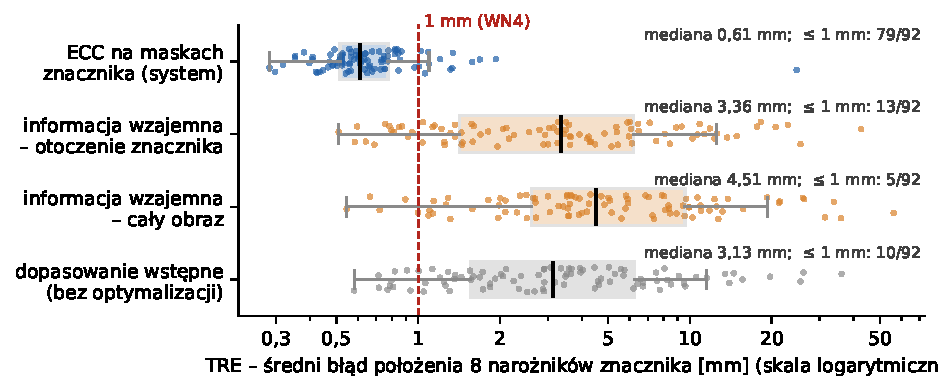
\includegraphics[width=0.92\textwidth]{rysunki/wyk_e4_tre.pdf}
  \caption{Błąd TRE czterech metod rejestracji w badaniu E4 ($n = 92$ pary); punkty -- pary, prostokąt -- kwartyle, czarna linia -- mediana. Źródło: opracowanie własne}
  \label{fig:e4}
\end{figure}

Mediana czasu rejestracji metodą zastosowaną w systemie wyniosła 8,4~s (maksymalnie 13,2~s), wobec 10,5~s i 16,0~s dla wariantów informacji wzajemnej; wymaganie WN1 zostało spełnione. % TODO: dopisać procesor i pamięć komputera, na którym mierzono czasy.

\section{Jakość segmentacji w obu modalnościach}
\label{sec:wyniki-segmentacja}

Jakość segmentacji oceniono względem masek z programu CVAT (tab.~\ref{tab:segmentacja}, rys.~\ref{fig:segmentacja}). Model M3 w 5-krotnej walidacji krzyżowej według znamion uzyskał współczynnik Dice'a 0,969 $\pm$ 0,008 (minimum 0,937), a wartości w poszczególnych foldach mieściły się w zakresie 0,968--0,970. Współczynnik Dice'a był nie mniejszy niż 0,9 dla wszystkich 94 obrazów, więc wymaganie WN5 zostało spełnione. Model zachowuje pole znacznika (stosunek pól 1,004), a mediana HD95 wynosi 0,62~mm, czyli około dwa piksele obrazu termowizyjnego. Detektor klasyczny z modułu rejestracji uzyskał mniejszy współczynnik Dice'a (0,954 $\pm$ 0,017; test Wilcoxona, $p < 0{,}001$) i zaniżał pole folii (stosunek pól 0,950), co uzasadnia zastosowanie modelu uczonego jako niezależnego punktu odniesienia w badaniu E2.

\begin{table}[htbp]
  \centering
  \caption{Segmentacja względem adnotacji z CVAT: średnia $\pm$ odchylenie standardowe (mediana)}
  \label{tab:segmentacja}
  \small
  \begin{tabular}{lccc}
    \toprule
    Miara & \makecell{M1 -- znamię,\\ zdjęcie ($n = 92$)} & \makecell{M3 -- znacznik,\\ termowizja ($n = 94$)} & \makecell{detektor klasyczny,\\ termowizja ($n = 94$)} \\
    \midrule
    Dice & 0,870 $\pm$ 0,103 (0,896) & 0,969 $\pm$ 0,008 (0,970) & 0,954 $\pm$ 0,017 (0,959) \\
    IoU & 0,782 $\pm$ 0,129 (0,812) & 0,939 $\pm$ 0,015 (0,941) & 0,913 $\pm$ 0,031 (0,921) \\
    HD95 [mm] & 0,38 $\pm$ 0,53 (0,24) & 0,68 $\pm$ 0,27 (0,62) & 1,06 $\pm$ 0,59 (0,83) \\
    ASSD [mm] & 0,15 $\pm$ 0,22 (0,10) & 0,23 $\pm$ 0,06 (0,22) & 0,32 $\pm$ 0,12 (0,31) \\
    stosunek pól & 1,22 $\pm$ 0,59 (1,10) & 1,004 $\pm$ 0,030 (1,006) & 0,950 $\pm$ 0,044 (0,951) \\
    \bottomrule
  \end{tabular}
\end{table}

% OPCJA (ok. 0,4 s.): wykres powtarza dane z tab. tab:segmentacja w postaci rozkładów -- przy braku miejsca usuń.
\begin{figure}[htbp]
  \centering
  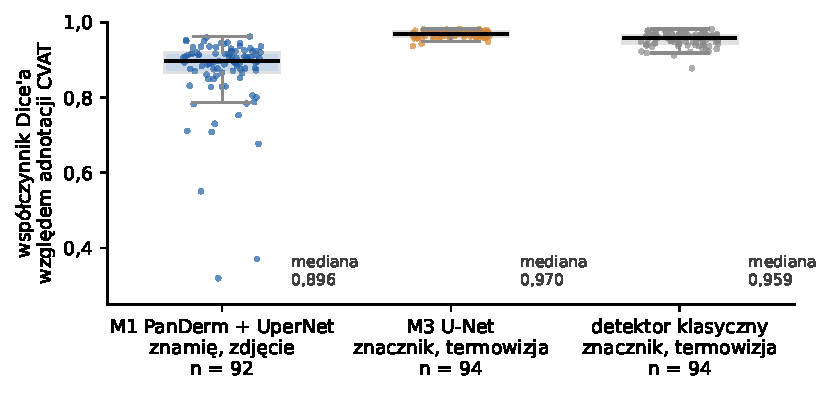
\includegraphics[width=0.85\textwidth]{rysunki/wyk_segmentacja.pdf}
  \caption{Współczynnik Dice'a segmentacji względem adnotacji z CVAT; punkty -- pary obrazów. Źródło: opracowanie własne}
  \label{fig:segmentacja}
\end{figure}

Model M1 na zdjęciach z telefonu uzyskał współczynnik Dice'a 0,870 $\pm$ 0,103 (mediana 0,896), a więc niewiele mniejszy niż na zbiorze testowym ISIC (0,899), mimo przesunięcia dziedziny. W 81 z 92 par współczynnik był nie mniejszy niż 0,8. Najsłabsze wyniki dotyczyły znamion położonych przy krawędzi folii lub w jej cieniu (pary 57 i 81: 0,32 i 0,37) oraz bardzo bladego znamienia (para 59: 0,55). Mediana stosunku pól równa 1,10 oznacza, że model systematycznie zawyża obszar znamienia, głównie przez szerszy niż w adnotacji brzeg. Znamiona są małe (mediana średnicy 2,1~mm), a dla małych struktur miary pokrycia są bardzo wrażliwe na błąd pojedynczych pikseli~\cite{maierhein2024}; dlatego obok współczynnika Dice'a podano miary odległościowe, z których wynika, że typowe przesunięcie brzegu maski (mediana ASSD) wynosi 0,10~mm.

\section{Zgodność obszaru zainteresowania między modalnościami}
\label{sec:wyniki-e2}

Badanie E2 nie wymaga adnotacji, dlatego system wykonuje je dla każdej analizowanej pary. Maska folii ze zdjęcia, przeniesiona macierzą $T$, pokrywała się z maską z modelu M3 ze współczynnikiem Dice'a 0,957 $\pm$ 0,032 (mediana 0,966), a w 89 z 92 par współczynnik był nie mniejszy niż 0,9 (tab.~\ref{tab:e1-e2}, kolumna E2). Dla otworu znacznika, czyli obszaru zainteresowania, mediana współczynnika Dice'a wyniosła 0,960, mediana HD95 -- 0,88~mm, a mediana przesunięcia środków -- 0,23~mm. Przykład dla pary 14 przedstawiono na rysunku~\ref{fig:wyniki-para}.

\begin{figure}[htbp]
  \centering
  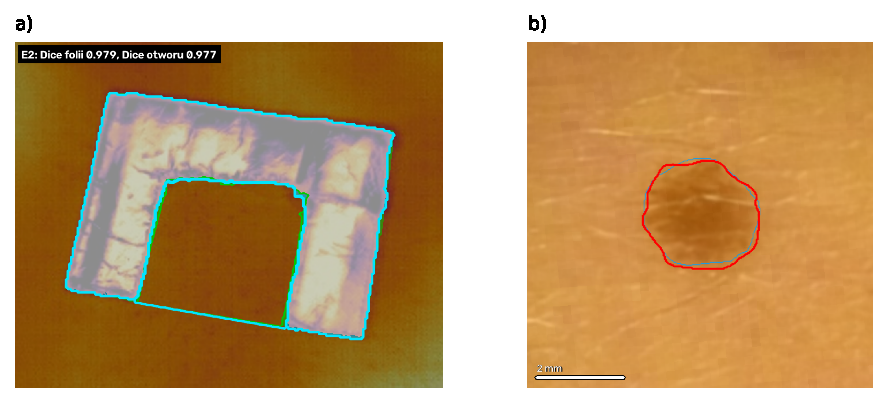
\includegraphics[width=0.9\textwidth]{rysunki/wyniki_para14.pdf}
  \caption{Para 14: a)~maska folii ze zdjęcia przeniesiona macierzą $T$ i maska z modelu M3 (biały -- obie maski, zielony -- tylko ze zdjęcia, turkusowy -- tylko M3), b)~nałożenie obrazu termowizyjnego na zdjęcie w otoczeniu znamienia: maska M1 (czerwona) i adnotacja z CVAT (niebieska); widoczne kwadraty to piksele kamery termowizyjnej. Źródło: opracowanie własne}
  \label{fig:wyniki-para}
\end{figure}

Najważniejszą właściwością badania E2 jest to, że wykrywa ono nieudaną rejestrację bez wzorca. Współczynnik Dice'a folii w badaniu E2 jest silnie skorelowany z błędem TRE wyznaczonym względem adnotacji ($\rho = -0{,}72$; rys.~\ref{fig:e2-tre}). Najmniejsze wartości wystąpiły w parach o największym błędzie rejestracji: 78 (Dice 0,72, TRE 24,7~mm), 8 (0,86; 2,3~mm) i 79 (0,89; 1,9~mm). Współczynnik Dice'a otworu mniejszy niż 0,93 wystąpił w 10 parach, z których 9 miało TRE większe niż 1~mm. Trafne okazało się też ostrzeżenie o niepewnej detekcji znacznika: wszystkie cztery pary, w których zgodność kształtu znacznika na zdjęciu z wzorcem była mniejsza niż 0,65 (pary 8, 59, 78 i 79), miały TRE większe niż 1,3~mm. Badanie E2 ujawnia również błędy segmentacji w jednej z modalności: w parze 1 maska folii ze zdjęcia wchodziła w otwór znacznika, co obniżyło współczynnik Dice'a otworu do 0,81 przy poprawnej rejestracji.

\begin{figure}[htbp]
  \centering
  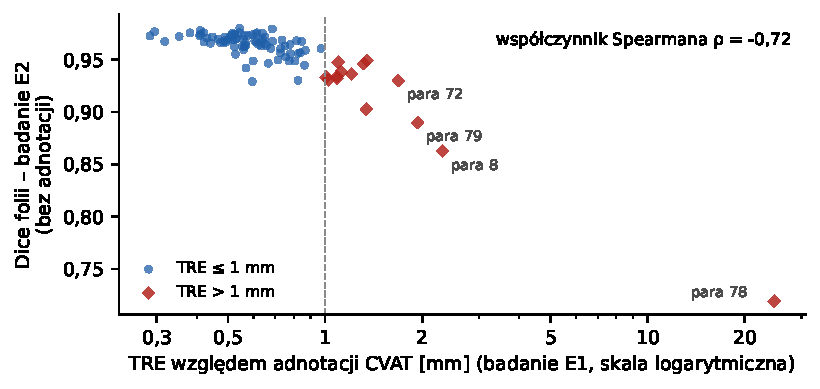
\includegraphics[width=0.9\textwidth]{rysunki/wyk_e2_tre.pdf}
  \caption{Współczynnik Dice'a folii w badaniu E2 (bez adnotacji) a błąd TRE względem adnotacji (badanie E1), $n = 92$ pary. Źródło: opracowanie własne}
  \label{fig:e2-tre}
\end{figure}

\section{Parametry znamion i piksele na obrazie termowizyjnym}
\label{sec:wyniki-piksele}

Parametry znamion zmierzone przez system oraz charakterystykę pikseli znamion na obrazie termowizyjnym zestawiono w tabeli~\ref{tab:znamiona}. Znamiona w zbiorze były małe: mediana pola wyniosła 3,4~mm$^2$, a średnicy równoważnej -- 2,1~mm. Stosunek pola znamienia przeniesionego na obraz termowizyjny do pola zmierzonego na zdjęciu wyniósł 1,015 $\pm$ 0,034. Oba pola obliczono niezależnymi homografiami, więc wynik bliski jedności potwierdza spójność skali i rejestracji.

\begin{table}[htbp]
  \centering
  \caption{Parametry znamion i piksele znamion na obrazie termowizyjnym ($n = 92$)}
  \label{tab:znamiona}
  \small
  \begin{tabular}{lcc}
    \toprule
    Wielkość & Mediana & Min.--maks. \\
    \midrule
    pole znamienia, model M1 [mm$^2$] & 3,42 & 1,16--28,58 \\
    pole znamienia, adnotacja CVAT [mm$^2$] & 3,24 & 0,97--28,09 \\
    średnica równoważna [mm] & 2,09 & 1,22--6,03 \\
    maksymalna średnica Fereta [mm] & 2,65 & 1,40--8,48 \\
    kolistość & 0,819 & 0,237--0,867 \\
    pole na obrazie termowizyjnym / pole na zdjęciu & 1,020 & 0,767--1,069 \\
    piksele w masce znamienia & 44 & 10--290 \\
    piksele pokryte częściowo (ułamek $< 0{,}5$) & 12 & 3--38 \\
    odchylenie standardowe intensywności w znamieniu [j.s.] & 14,1 & 6,0--68,4 \\
    rozstęp intensywności w znamieniu [j.s.] & 65 & 27--333 \\
    \bottomrule
  \end{tabular}
  \\[2pt]{\footnotesize j.s. -- jednostki surowe detektora (wartości z nagrania .SEQ)}
\end{table}

Dla 92 znamion zapisano łącznie 7337 pikseli należących do masek oraz piksele pokryte częściowo, wraz ze współrzędnymi i surową intensywnością (WF15). Przykład przedstawiono na rysunku~\ref{fig:piksele}. Zmienność intensywności w obrębie znamienia była niewielka: mediana odchylenia standardowego wyniosła 14,1 jednostek surowych. Na podstawie map temperatur wyznaczonych z parametrów kamery jednej jednostce stopnia Celsjusza odpowiada w zakresie temperatur skóry (30--37~°C) około 213 jednostek surowych, więc odchylenie to odpowiada około 0,07~°C. Wynik ten jest zgodny z obserwacją, że bez schłodzenia skóry znamię nie wyróżnia się na obrazie termowizyjnym~\cite{visualization-detection-cancer}. Należy też pamiętać, że przy medianie błędu rejestracji około dwóch pikseli kamery piksele brzegowe mogą obejmować skórę wokół znamienia; dlatego dla każdego piksela zapisywany jest ułamek pokrycia.

\begin{figure}[htbp]
  \centering
  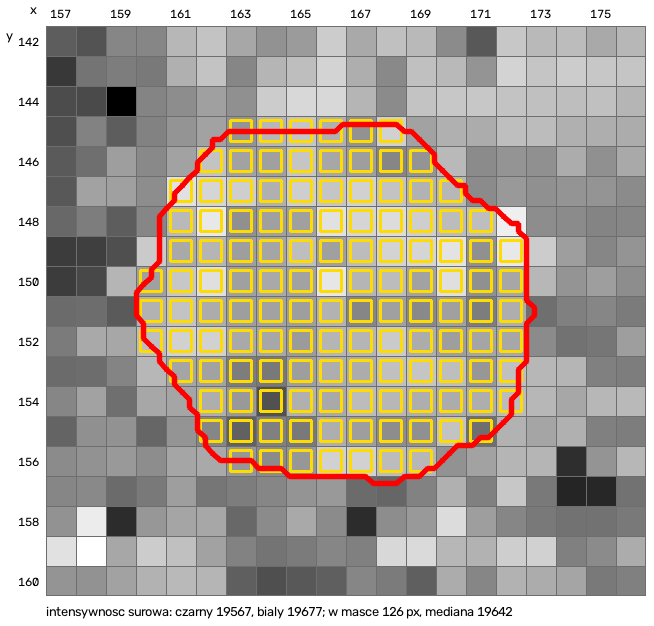
\includegraphics[width=0.5\textwidth]{rysunki/piksele_para14.png}
  \caption{Piksele obrazu termowizyjnego objęte znamieniem w parze 14: surowa intensywność z nagrania (skala szarości rozciągnięta w kadrze), znamię przeniesione ze zdjęcia (czerwona linia) i piksele w masce (żółte ramki); na brzegach współrzędne $x$ i $y$ pikseli. Źródło: opracowanie własne}
  \label{fig:piksele}
\end{figure}

\section{Testy funkcjonalne}
\label{sec:testy-funkcjonalne}

Spełnienie wymagań funkcjonalnych i części wymagań pozafunkcjonalnych sprawdzono 18 testami automatycznymi napisanymi z użyciem modułu \texttt{unittest} (tab.~\ref{tab:testy}). Testy wykonują etapy systemu bez interfejsu graficznego na danych ze zbioru (para 14 z adnotacjami i para 75 z niewykrywalnym znacznikiem) oraz na danych przygotowanych w teście, a wyniki zapisują w folderach tymczasowych i osobnej bazie danych. Zaliczono 17 testów; test T09 pominięto, ponieważ w środowisku testowym nie było wag modelu M3. Czas wykonania całego zestawu wyniósł około 20~s. % TODO: uruchom projekt/testy/uruchom_testy.bat i wpisz wynik (w maszynie bez wag U-Net: 17 zaliczonych, T09 pominięty).

\begin{table}[htbp]
  \centering
  \caption{Testy funkcjonalne systemu}
  \label{tab:testy}
  \footnotesize
  \begin{tabularx}{\textwidth}{l l X l}
    \toprule
    ID & Wymaganie & Sprawdzane zachowanie & Wynik \\
    \midrule
    T01 & WF1 & wczytanie pary ze zbioru: obrazy, numer znamienia, adnotacje & zaliczony \\
    T02 & WF1, WN6 & nieistniejący plik -- komunikat zamiast awarii & zaliczony \\
    T03 & WN6 & etap wywołany przed poprzednim -- komunikat & zaliczony \\
    T04 & WF2, WN1, WN4 & pełna rejestracja pary 14: czas 6,4~s, TRE 0,69~mm & zaliczony \\
    T05 & WN6 & obraz termowizyjny bez znacznika -- ostrzeżenie (zgodność z $\Pi$ 0,54) & zaliczony \\
    T06 & WN6 & para 75 -- znacznik niezgodny z wzorcem odrzucony z komunikatem & zaliczony \\
    T07 & WF4 & 8 narożników w obu modalnościach, IoU wzorca $\geq 0{,}8$ & zaliczony \\
    T08 & WF7, WF8 & pole znamienia na obu obrazach zgodne ($\pm$15\%), komplet parametrów & zaliczony \\
    T09 & WF6, WF9 & maska M3 i miary E2 (Dice folii $\geq 0{,}9$) & pominięty$^{*}$ \\
    T10 & WF15 & współrzędne i surowa intensywność pikseli zgodne z nagraniem & zaliczony \\
    T11 & WF15 & zapis pikseli do CSV i odczyt bez utraty danych & zaliczony \\
    T12 & WF15, WN6 & brak nagrania .SEQ -- analiza bez pikseli, uwaga w raporcie & zaliczony \\
    T13 & WF15 & własne pliki z nagraniem .SEQ -- odczyt intensywności & zaliczony \\
    T14 & WF11 & raport HTML, \texttt{metryki.json}, obrazy PNG i CSV pikseli & zaliczony \\
    T15 & WF12, WN9 & zapis analizy, miar i pikseli w bazie & zaliczony \\
    T16 & WF12 & migracja bazy ze starszej wersji schematu & zaliczony \\
    T17 & WF9 & miary zgodności na maskach o znanym wyniku & zaliczony \\
    T18 & WF7 & przeniesienie punktów i ułamek pokrycia pikseli & zaliczony \\
    \bottomrule
  \end{tabularx}
  \\[2pt]{\footnotesize $^{*}$ wymaga wag modelu M3, niedostępnych w środowisku testowym; % TODO: po uruchomieniu uruchom_testy.bat na komputerze autora wpisać wynik
}
\end{table}

Działanie interfejsu graficznego sprawdzono ręcznie według scenariuszy: wczytanie pary ze zbioru i własnych plików (TG1), wykonanie wszystkich etapów jednym poleceniem (TG2), praca krok po kroku z kontrolą aktywności przycisków (TG3), regulacja przezroczystości i zapis nałożenia (TG4), wyświetlanie objaśnień wielkości (TG5) oraz zapis i otwarcie raportu wraz z podglądem obrazów (TG6). % TODO: wykonać TG1–TG6 i wpisać wynik (np. „Wszystkie scenariusze zakończyły się zgodnie z oczekiwaniami.”).

\section{Dyskusja i ograniczenia}
\label{sec:dyskusja}

Zastosowanie znacznika widocznego w obu modalnościach i maksymalizacja kryterium ECC na maskach zamiast na intensywnościach zmniejszyły medianę błędu rejestracji około pięciokrotnie względem informacji wzajemnej. Bezpośrednie porównanie z wynikami innych prac jest ograniczone, ponieważ stosowano w nich inne dane i miary: błąd w pikselach przy rejestracji z szablonem kalibracyjnym~\cite{non-contact-breathing-monitoring}, zgodność masek dużych obiektów (stóp)~\cite{gonzalezperez2021} albo miary podobieństwa obrazów bez błędu położenia punktów w milimetrach~\cite{oniga2026}. W niniejszej pracy błąd rejestracji wyrażono w milimetrach na płaszczyźnie znacznika, a dodatkowo zastosowano niezależną kontrolę bez adnotacji (E2), która pozwala wskazać pary wymagające sprawdzenia.

Ograniczenia przeprowadzonych badań są następujące:
\begin{itemize}
  \item dane pochodzą z jednej serii pomiarowej, jednego zestawu urządzeń i jednej osoby wykonującej zdjęcia, a adnotacje wykonał jeden oznaczający -- zgodność ekspertów przy oznaczaniu znamion jest ograniczona~\cite{codella2019};
  \item model przekształcenia zakłada, że skóra w obrębie znacznika jest płaska; znacznik musi w całości znajdować się w kadrze obu urządzeń;
  \item obraz termowizyjny bez znacznika powoduje ostrzeżenie, ale nie przerywa rejestracji (test T05) -- decyzję podejmuje użytkownik na podstawie uwag w raporcie;
  \item model M1 zawyża pole znamienia (mediana stosunku pól 1,10), a jego jakość na zdjęciach z telefonu oceniono tylko na 92 parach;
  \item intensywność pikseli jest surową wartością detektora, bez kalibracji temperatury i bez schłodzenia skóry, więc nie pozwala ocenić termicznych właściwości znamienia.
\end{itemize}

% =====================================================================
% Rozdział 7 – Podsumowanie (WZÓR, ok. 1,5 strony)
% Styl bezosobowy; bez nowych wyników. Plan i zwroty: materialy/06_plan_zwroty_rozdzialy_4_7.md.
% =====================================================================

\chapter{Podsumowanie}
\label{chap:podsumowanie}

\section{Realizacja celu pracy}
\label{sec:realizacja}

Celem pracy było opracowanie, implementacja oraz ocena systemu umożliwiającego rejestrację i wspólną analizę zdjęcia RGB wykonanego telefonem i obrazu termowizyjnego zmiany skórnej. Cel ten został osiągnięty, a zadania wymienione w podrozdziale~\ref{sec:cel} zrealizowano w następujący sposób:
\begin{itemize}
  \item na podstawie przeglądu literatury przyjęto rejestrację opartą na znaczniku widocznym w obu modalnościach i ocenę błędem TRE oraz miarami zgodności masek;
  \item zaprojektowano system w architekturze potokowej (przypadki użycia, architektura, diagram klas, interfejs) oraz bazę danych SQLite z sześcioma tabelami, przechowującą zbiór, adnotacje, wyniki analiz i piksele znamion;
  \item zaprojektowano znacznik $\Pi$, zebrano zbiór 94 par obrazów 34 znamion i wykonano ich adnotacje;
  \item zaimplementowano moduł rejestracji, modele segmentacji dla obu modalności (M1 -- znamię na zdjęciu, M3 -- znacznik na obrazie termowizyjnym), przeniesienie obszarów z pomiarami w milimetrach, miary zgodności oraz zapis współrzędnych i surowej intensywności pikseli znamienia;
  \item przygotowano aplikację z interfejsem graficznym, przetwarzanie wsadowe i raporty;
  \item przeprowadzono weryfikację systemu (badania E1, E2, E4, ocena segmentacji, testy funkcjonalne) oraz przygotowano instrukcję użytkownika i dokumentację techniczną (Dodatki~A i~B).
\end{itemize}
Wszystkie wymagania funkcjonalne o priorytecie \emph{wymagane} zostały zrealizowane, a kryteria akceptacji wymagań pozafunkcjonalnych WN1, WN4 i WN5 -- spełnione.

\section{Wnioski}
\label{sec:wnioski}

Najważniejsze wnioski z pracy są następujące:
\begin{enumerate}
  \item Znacznik referencyjny widoczny w obu modalnościach pozwala zarejestrować zdjęcie z telefonu i obraz termowizyjny z niezależnych urządzeń z medianą błędu 0,61~mm, czyli około dwóch pikseli kamery termowizyjnej; w 85\% par błąd nie przekroczył 1~mm.
  \item Maksymalizacja kryterium ECC na maskach znacznika jest wyraźnie dokładniejsza od rejestracji na intensywnościach z użyciem informacji wzajemnej (mediana TRE 0,61~mm wobec 3,36~mm), ponieważ nie zależy od związku między intensywnościami obu modalności.
  \item Niewielka sieć U-Net uczona na 94 obrazach wystarcza do segmentacji znacznika na obrazie termowizyjnym (współczynnik Dice'a 0,969), a porównanie jej maski z maską przeniesioną ze zdjęcia (badanie E2) pozwala bez adnotacji wskazać pary z nieudaną rejestracją.
  \item Model bazowy douczony na obrazach dermatoskopowych może segmentować znamiona na zdjęciach z telefonu (współczynnik Dice'a 0,870) pod warunkiem ograniczenia obszaru do wnętrza znacznika i doboru kadru zgodnego z danymi uczącymi; model zawyża jednak pole znamienia.
  \item System dostarcza dla każdego znamienia listę pikseli obrazu termowizyjnego z ich współrzędnymi i surową intensywnością. W obrazach statycznych, wykonanych bez schłodzenia skóry, zmienność intensywności w obrębie znamienia jest niewielka (około 0,07~°C), co uzasadnia rozszerzenie badań o termografię dynamiczną.
\end{enumerate}

\section{Kierunki dalszych prac}
\label{sec:dalsze-prace}

Ograniczenia opisane w podrozdziale~\ref{sec:dyskusja} wyznaczają kierunki dalszych prac:
\begin{itemize}
  \item rozszerzenie systemu o termografię dynamiczną -- rejestrację sekwencji obrazów po schłodzeniu skóry i analizę zmian intensywności pikseli znamienia w czasie;
  \item douczenie modelu M1 na zdjęciach z telefonu z walidacją krzyżową według znamion, aby ograniczyć zawyżanie pola znamienia;
  \item przerywanie analizy, gdy znacznik na obrazie termowizyjnym jest wykryty niepewnie, oraz automatyczne oznaczanie par z niską zgodnością w badaniu E2;
  \item zebranie kolejnych serii pomiarowych z udziałem większej liczby osób, urządzeń i oznaczających, co pozwoli ocenić zmienność adnotacji i uogólnienie modeli;
  \item przeliczanie intensywności na temperaturę z kalibracją kamery oraz ocena użyteczności systemu z udziałem lekarzy.
\end{itemize}

\bibliographystyle{acm}
\bibliography{literatura_wzor}
\appendix
% =====================================================================
% Dodatek A – Instrukcja użytkownika (WZÓR, ok. 2 strony)
% Wstaw po \appendix. Zrzuty ekranu do wykonania – lista w materialy/07_plan_dodatki_streszczenie_skroty.md.
% Plan i zwroty: materialy/07_plan_dodatki_streszczenie_skroty.md.
% =====================================================================

\chapter{Instrukcja użytkownika}
\label{app:instrukcja}

Instrukcja opisuje analizę pary obrazów zmiany skórnej w aplikacji okienkowej systemu. Instalację środowisk opisano w dokumentacji technicznej (Dodatek~\ref{app:dokumentacja}).

\section{Uruchomienie}

Aplikację uruchamia się w systemie Windows poleceniem:
\begin{center}
\texttt{inzynierka\textbackslash Scripts\textbackslash python.exe projekt\textbackslash aplikacja.py}
\end{center}
wydanym w folderze głównym projektu. Segmentacja znamienia wymaga zainstalowanego środowiska modeli; pozostałe etapy działają bez niego.

\section{Przygotowanie obrazów}

Przed wykonaniem zdjęć należy nakleić znacznik $\Pi$ tak, aby znamię znajdowało się między jego ramionami, w otworze znacznika. Znacznik musi w całości mieścić się w kadrze zarówno telefonu, jak i kamery termowizyjnej. Zdjęcie należy wykonać możliwie prostopadle do skóry, bez lampy błyskowej i bez silnych odblasków na folii. Z kamery termowizyjnej zapisuje się nagranie .SEQ; aby system zapisał intensywność pikseli znamienia, obraz termowizyjny (JPG) i nagranie muszą mieć tę samą nazwę i leżeć w tym samym folderze. Dla par ze zbioru nagrania są przypisane automatycznie.

\section{Analiza pary krok po kroku}

Okno aplikacji (rys.~\ref{fig:interfejs}) składa się z paska sześciu etapów, panelu sterowania po lewej stronie, podglądów obrazów po prawej oraz paska stanu z dziennikiem zdarzeń. Kółko myszy powiększa podgląd, przeciąganie przesuwa obraz, a dwukrotne kliknięcie przywraca widok początkowy. Przyciski etapów, których nie można jeszcze wykonać, są nieaktywne. Kolejne kroki analizy przedstawiono w tabeli~\ref{tab:instrukcja-kroki}. Wszystkie etapy można też wykonać jednym poleceniem \emph{Wykonaj wszystkie etapy} w zakładce \emph{1. Dane}; po jego zakończeniu aplikacja przechodzi do zakładki raportu.

\begin{table}[!ht]
  \centering
  \caption{Analiza pary obrazów w aplikacji}
  \label{tab:instrukcja-kroki}
  \footnotesize
  \begin{tabularx}{\textwidth}{>{\raggedright\arraybackslash}p{2.3cm} X X}
    \toprule
    Zakładka & Czynność użytkownika & Wynik \\
    \midrule
    1. Dane & wybrać \emph{Para z bazy}, numer pary (przyciski ze strzałkami zmieniają parę) i kliknąć \emph{Wczytaj parę}; albo wybrać \emph{Własne pliki}, wskazać zdjęcie i obraz termowizyjny i kliknąć \emph{Wczytaj pliki} & podgląd obu obrazów; informacje o parze, adnotacjach i nagraniu .SEQ \\
    2. Rejestracja & kliknąć \emph{Uruchom rejestrację} (lub \emph{Wczytaj zapisaną rejestrację}); suwakiem ustawić przezroczystość; opcjonalnie \emph{Zapisz nałożenie\ldots} & nałożenie obrazów, model przekształcenia, kontury znacznika z obu modalności \\
    3. Segmentacja & kliknąć \emph{Wyznacz narożniki, znamię i znacznik na termowizji} & narożniki 0--7, maska znamienia na zdjęciu, maska znacznika na obrazie termowizyjnym \\
    4. Przeniesienie ROI & kliknąć \emph{Przenieś na termowizję}; przełączyć widok zdjęcia (\emph{Zdjęcie} / \emph{Nałożenie}) & znamię i znacznik na obrazie termowizyjnym \\
    5. Pomiary & kliknąć \emph{Oblicz pomiary i zgodność}; kliknąć nazwę wielkości w tabeli, aby wyświetlić jej objaśnienie & tabela wyników (badanie E2, kontrola skali, parametry znamienia, piksele znamienia) oraz uwagi \\
    6. Raport & kliknąć \emph{Zapisz raport}, następnie \emph{Otwórz raport} lub \emph{Otwórz folder wyników}; przełączać podgląd obrazów raportu & pliki raportu (tab.~\ref{tab:instrukcja-pliki}) \\
    \bottomrule
  \end{tabularx}
\end{table}

% TODO: zrzut zakładki „5. Pomiary” (para 14, sekcja „Piksele znamienia na termowizji”) – rysunek opcjonalny:
% \begin{figure}[htbp]
%   \centering
%   \includegraphics[width=\textwidth]{rysunki/interfejs_pomiary.png}
%   \caption{Zakładka pomiarów: tabela wyników i objaśnienie wybranej wielkości}
%   \label{fig:interfejs-pomiary}
% \end{figure}

\section{Wyniki}

Wyniki zapisywane są w folderze \texttt{wyniki\textbackslash wyniki\_obu\textbackslash para\_N} (dla własnych plików -- w folderze nazwanym od nazw plików), który można zmienić w zakładce raportu. Zawartość folderu opisano w tabeli~\ref{tab:instrukcja-pliki}. Raport otwiera się w dowolnej przeglądarce; na jego początku znajdują się uwagi wymagające sprawdzenia, a na końcu objaśnienia wszystkich wielkości.

\begin{table}[!ht]
  \centering
  \caption{Pliki wynikowe analizy pary}
  \label{tab:instrukcja-pliki}
  \footnotesize
  \begin{tabularx}{\textwidth}{>{\raggedright\arraybackslash}p{4.4cm} X}
    \toprule
    Plik & Zawartość \\
    \midrule
    \texttt{raport.html} & raport z obrazami, tabelami wyników, uwagami i objaśnieniami \\
    \texttt{metryki.json} & wszystkie wyniki liczbowe (do dalszej analizy) \\
    \texttt{rgb.png}, \texttt{termal.png}, \texttt{nakladka.png}, \texttt{nakladka\_zblizenie.png}, \texttt{znacznik\_modalnosci.png}, \texttt{piksele\_termal.png} & obrazy raportu: zdjęcie i obraz termowizyjny z obrysami, nałożenie, powiększenie wokół znamienia, maski badania E2, piksele znamienia \\
    \texttt{piksele\_znamienia\_termal.csv} & piksele znamienia na obrazie termowizyjnym: \texttt{x}, \texttt{y} (kolumna i wiersz), \texttt{ulamek} (pokrycie piksela przez znamię), \texttt{w\_masce} (1 -- pokrycie co najmniej 50\%), \texttt{intensywnosc} (surowa wartość z nagrania .SEQ); separator średnik \\
    \bottomrule
  \end{tabularx}
\end{table}

\section{Komunikaty i rozwiązywanie problemów}

Najczęstsze komunikaty i sposób postępowania przedstawiono w tabeli~\ref{tab:instrukcja-bledy}. Komunikaty błędów wyświetlane są w oknie dialogowym, a ich szczegóły -- w dzienniku zdarzeń.

\begin{table}[!ht]
  \centering
  \caption{Komunikaty systemu i sposób postępowania}
  \label{tab:instrukcja-bledy}
  \footnotesize
  \begin{tabularx}{\textwidth}{>{\raggedright\arraybackslash}p{4.2cm} X X}
    \toprule
    Komunikat lub uwaga & Przyczyna & Postępowanie \\
    \midrule
    \emph{Nie można otworzyć zdjęcia / obrazu termowizyjnego} & plik nie istnieje lub ma nieobsługiwany format & wskazać plik JPG lub PNG \\
    \emph{Nie znaleziono znacznika}, \emph{znacznik wykryty niepewnie} & znacznik ucięty przez kadr, zasłonięty lub z silnym odblaskiem & sprawdzić nałożenie; w razie błędu powtórzyć zdjęcie \\
    \emph{Najpierw wykonaj \ldots} & pominięto wcześniejszy etap & wykonać etapy w kolejności zakładek \\
    \emph{Nie ma środowiska modeli z PyTorch} & brak środowiska modelu M1 & zainstalować środowisko modeli (Dodatek~\ref{app:dokumentacja}) \\
    \emph{Brak surowej intensywności termowizji} & brak nagrania .SEQ o tej samej nazwie co obraz & umieścić nagranie obok obrazu i powtórzyć pomiary \\
    niska zgodność masek między modalnościami (E2) lub błąd narożników powyżej 1~mm & możliwy błąd rejestracji lub segmentacji & ocenić nałożenie; wyników pary nie używać bez sprawdzenia \\
    \bottomrule
  \end{tabularx}
\end{table}

% =====================================================================
% Dodatek B – Dokumentacja techniczna (WZÓR, ok. 2 strony)
% Wstaw po dodatku A. Wymaga pakietów: booktabs, tabularx, listings (listingi B.1, B.2).
% Plan i zwroty: materialy/07_plan_dodatki_streszczenie_skroty.md.
% =====================================================================

\chapter{Dokumentacja techniczna}
\label{app:dokumentacja}

Dokumentacja jest przeznaczona dla osoby instalującej, utrzymującej lub rozwijającej system. Kod źródłowy znajduje się w folderze \texttt{projekt}, a szczegółowe opisy -- w plikach \texttt{README.md} folderów \texttt{projekt} i \texttt{projekt/modele\_segmentacja}.

\section{Środowiska i instalacja}

System korzysta z dwóch środowisk języka Python (tab.~\ref{tab:srodowiska}). Środowisko aplikacji jest lekkie i nie zawiera biblioteki PyTorch; środowisko modeli służy do segmentacji znamienia modelem M1, uczenia modeli oraz przetwarzania wsadowego. Ścieżki środowiska modeli, wag i zbiorów danych zdefiniowano w module \texttt{modele\_segmentacja/konfiguracja.py}; katalog bazowy można zmienić zmienną środowiskową \texttt{MODELE\_DANE}.

\begin{table}[!ht]
  \centering
  \caption{Środowiska uruchomieniowe systemu}
  \label{tab:srodowiska}
  \footnotesize
  \begin{tabularx}{\textwidth}{>{\raggedright\arraybackslash}p{2.2cm} >{\raggedright\arraybackslash}X >{\raggedright\arraybackslash}X}
    \toprule
    & Środowisko aplikacji & Środowisko modeli \\
    \midrule
    położenie & \texttt{inzynierka\textbackslash} (folder główny projektu) & \texttt{\%USERPROFILE\%\textbackslash modele\_dane\textbackslash srodowisko\textbackslash} \\
    Python & 3.14 & 3.12 \\
    biblioteki & customtkinter, OpenCV, NumPy, Pillow, flirpy, matplotlib; SimpleITK (tylko badanie E4) & PyTorch 2.11 z CUDA 12.8, torchvision, OpenCV, NumPy, bitsandbytes, SimpleITK, onnx (lista: \texttt{modele\_segmentacja/wymagania\_srodowiska.txt}) \\
    zastosowanie & aplikacja, model M3 (ONNX), testy & model M1, uczenie modeli, potok wsadowy, raport zbiorczy \\
    \bottomrule
  \end{tabularx}
\end{table}

Instalacja środowiska aplikacji (w folderze głównym projektu):
\begin{verbatim}
py -3.14 -m venv inzynierka
inzynierka\Scripts\pip install customtkinter opencv-python numpy pillow ^
    flirpy matplotlib simpleitk
\end{verbatim}
Środowisko modeli tworzy się analogicznie z pliku \texttt{wymagania\_srodowiska.txt} (\texttt{pip install -r}). Wagi modeli umieszcza się w katalogu \texttt{modele\_dane\textbackslash wagi}: koder PanDerm i wytrenowany model M1 w podkatalogu modelu, a model M3 jako pliki \texttt{unet\_termal\textbackslash fold1.onnx}--\texttt{fold5.onnx} i \texttt{wszystkie.onnx}.

\section{Struktura kodu}

Etapy systemu zrealizowano w pakiecie \texttt{analiza}, wspólnym dla aplikacji i przetwarzania wsadowego (tab.~\ref{tab:moduly}). Modele segmentacji znajdują się w pakiecie \texttt{modele\_segmentacja}, a metoda rejestracji -- w module \texttt{dopasowanie3.py}.

\begin{table}[!ht]
  \centering
  \caption{Moduły pakietu \texttt{analiza} i główne moduły projektu}
  \label{tab:moduly}
  \footnotesize
  \begin{tabularx}{\textwidth}{>{\raggedright\arraybackslash}p{4.3cm} X}
    \toprule
    Moduł & Odpowiedzialność \\
    \midrule
    \texttt{analiza/system.py} & klasa \texttt{Analiza} (etapy potoku), wyjątek \texttt{BladEtapu}, funkcje \texttt{analizuj}, \texttt{analizuj\_z\_zapisanych} \\
    \texttt{analiza/dane.py} & dane par ze zbioru, adnotacje z CVAT, surowa intensywność z nagrań .SEQ \\
    \texttt{analiza/geometria.py} & przenoszenie punktów i masek macierzą $T$, ułamek pokrycia, skala mm/piksel \\
    \texttt{analiza/miary.py} & Dice, IoU, HD95, ASSD, przesunięcie środków, stosunek pól, TRE \\
    \texttt{analiza/pomiary.py} & parametry znamienia, piksele znamienia na obrazie termowizyjnym i ich zapis do CSV \\
    \texttt{analiza/obrazy.py}, \texttt{raport.py} & obrazy raportu i raport HTML z objaśnieniami \\
    \texttt{analiza/baza.py} & klasa \texttt{Baza} (SQLite), schemat, migracja, import i eksport \\
    \texttt{dopasowanie3.py} & detekcja znacznika, dopasowanie wstępne, ECC, wybór modelu przekształcenia \\
    \texttt{modele\_segmentacja/} & interfejs \texttt{ModelSegmentacji}, model M1, kandydaci na znamię, model M3 (\texttt{unet\_termal/}) \\
    \texttt{aplikacja.py} & interfejs graficzny (klasy \texttt{Aplikacja}, \texttt{Podglad}) \\
    \bottomrule
  \end{tabularx}
\end{table}

Klasa \texttt{Analiza} udostępnia metody odpowiadające etapom potoku, które należy wywoływać w kolejności przedstawionej na listingu~\ref{lst:analiza}. Wywołanie etapu bez wyniku poprzedniego kończy się wyjątkiem \texttt{BladEtapu} z opisem brakującego kroku.

\begin{lstlisting}[language=Python, caption={Analiza pary bez interfejsu graficznego}, label={lst:analiza}]
from analiza.system import Analiza
a = Analiza.z_pary(14)          # albo Analiza("zdjecie.jpg", "termal.jpg")
a.rejestruj()                   # macierz T
a.ustaw_narozniki()             # narozniki i skala mm
a.segmentuj_znamie()            # model M1 (srodowisko modeli)
a.segmentuj_znacznik_termal()   # model M3 (ONNX)
a.przenies(); a.zmierz()        # przeniesienie ROI, pomiary, piksele
print(a.zapisz_raport())        # raport, metryki.json, CSV, wpis w bazie
\end{lstlisting}

\section{Formaty danych}

Dane pary przechowywane są w folderze \texttt{dane/pary/N}: zdjęcie \texttt{rgb.jpg}, obraz termowizyjny \texttt{termal.jpg}, surowe wartości detektora \texttt{termal\_surowe.npy} (macierz 240~$\times$~320, \texttt{uint16}), mapa temperatur \texttt{termal\_C.npy}, maski z CVAT (PNG, 0/255) oraz \texttt{narozniki.json} z narożnikami i homografiami piksele--milimetry obu modalności. Wynik rejestracji zapisywany jest w folderze \texttt{wyniki/wyniki\_dopasowania/para\_N}, m.in. jako macierz $T$ w pliku tekstowym \texttt{dopasowanie\_macierz.txt} (3~$\times$~3, piksel zdjęcia $\to$ piksel obrazu termowizyjnego). Plik \texttt{metryki.json} zawiera wyniki pogrupowane według badań (\texttt{rejestracja}, \texttt{zgodnosc}, \texttt{zgodnosc\_modalnosci}, \texttt{pomiary\_rgb}, \texttt{kontrola\_skali}, \texttt{piksele\_termal} i in.), a format pliku pikseli opisano w tabeli~\ref{tab:instrukcja-pliki}.

\section{Baza danych}

Schemat bazy (rys.~\ref{fig:erd}) zdefiniowano w module \texttt{analiza/baza.py}. Numer wersji schematu jest zapisywany w polu \texttt{user\_version} pliku bazy (obecnie 2); przy otwarciu starszej bazy tworzone są brakujące tabele. Obsługę bazy z wiersza poleceń zapewnia skrypt \texttt{baza\_danych.bat} z poleceniami \texttt{utworz}, \texttt{importuj\_wyniki}, \texttt{pokaz}, \texttt{eksport}, \texttt{eksport\_piksele} i \texttt{sql}. Przykładowe zapytania przedstawiono na listingu~\ref{lst:sql}.

\begin{lstlisting}[language=SQL, caption={Przykładowe zapytania do bazy danych}, label={lst:sql}]
-- wspolczynnik Dice'a otworu (badanie E2) dla wszystkich par
SELECT para, wartosc FROM wyniki_par
 WHERE grupa = 'zgodnosc_modalnosci.otwor' AND nazwa = 'dice';
-- piksele znamienia pary 14 z ostatniej analizy
SELECT x, y, intensywnosc FROM piksel
 WHERE w_masce = 1 AND analiza_id =
   (SELECT id FROM ostatnia_analiza WHERE para_id = 14);
\end{lstlisting}

\section{Skrypty pomocnicze, uczenie i testy}

Skrypty wsadowe uruchamia się z folderu \texttt{projekt} (tab.~\ref{tab:skrypty}). Testy funkcjonalne (podrozdział~\ref{sec:testy-funkcjonalne}) uruchamia skrypt \texttt{testy/uruchom\_testy.bat}, który zapisuje wynik w pliku \texttt{testy/wynik\_testow.txt}.

\begin{table}[!ht]
  \centering
  \caption{Skrypty pomocnicze systemu}
  \label{tab:skrypty}
  \footnotesize
  \begin{tabularx}{\textwidth}{>{\raggedright\arraybackslash}p{5.0cm} X}
    \toprule
    Skrypt & Zadanie \\
    \midrule
    \texttt{potok\_pary.bat 1-94} [\texttt{--z\_zapisanych}] & analiza wskazanych par (z zapisaną rejestracją i maskami M1 -- bez GPU) \\
    \texttt{raport\_zbiorczy.bat} & raport zbiorczy wszystkich par i tabele \LaTeX{} \\
    \texttt{porownaj\_rejestracje.py} & badanie E4: porównanie metod rejestracji \\
    \texttt{read\_flirpy.py}, \texttt{heic\_do\_jpg.py} & konwersja nagrań .SEQ i zdjęć HEIC \\
    \texttt{temperatury\_par.py} [\texttt{--tylko\_surowe}] & mapy temperatur i surowe wartości detektora dla par \\
    \texttt{import\_cvat.py} & import adnotacji z programu CVAT \\
    \texttt{modele\_segmentacja/trenuj\_panderm.bat} & douczanie modelu M1 na zbiorze ISIC 2018 \\
    \texttt{modele\_segmentacja/trenuj\_unet\_termal.bat}, \texttt{ocen\_unet\_termal.bat} & uczenie modelu M3 (5 foldów i model końcowy) i jego ocena \\
    \bottomrule
  \end{tabularx}
\end{table}

\section{Rozszerzanie systemu}

Nowy model segmentacji znamienia dodaje się jako podkatalog \texttt{modele\_segmentacja/modele} z klasą \texttt{Model} dziedziczącą po \texttt{ModelSegmentacji}; model jest wykrywany automatycznie. Nowa miara dopisana do słownika wyników trafia automatycznie do pliku \texttt{metryki.json} i tabeli \texttt{miara}, bez zmiany schematu bazy. Parametry metody rejestracji -- model przekształcenia (\texttt{MODEL}), próg zgodności z wzorcem (\texttt{MIN\_ZGODNOSC}) i rozdzielczość roboczą zdjęcia (\texttt{RGB\_DET\_PX}) -- zdefiniowano jako stałe w module \texttt{dopasowanie3.py}.

\end{document}
